\chapter{Supplementary figures}
\label{app:figures}

% 3 - LOCUS CHAPTER

\begin{figure}
	\centering
	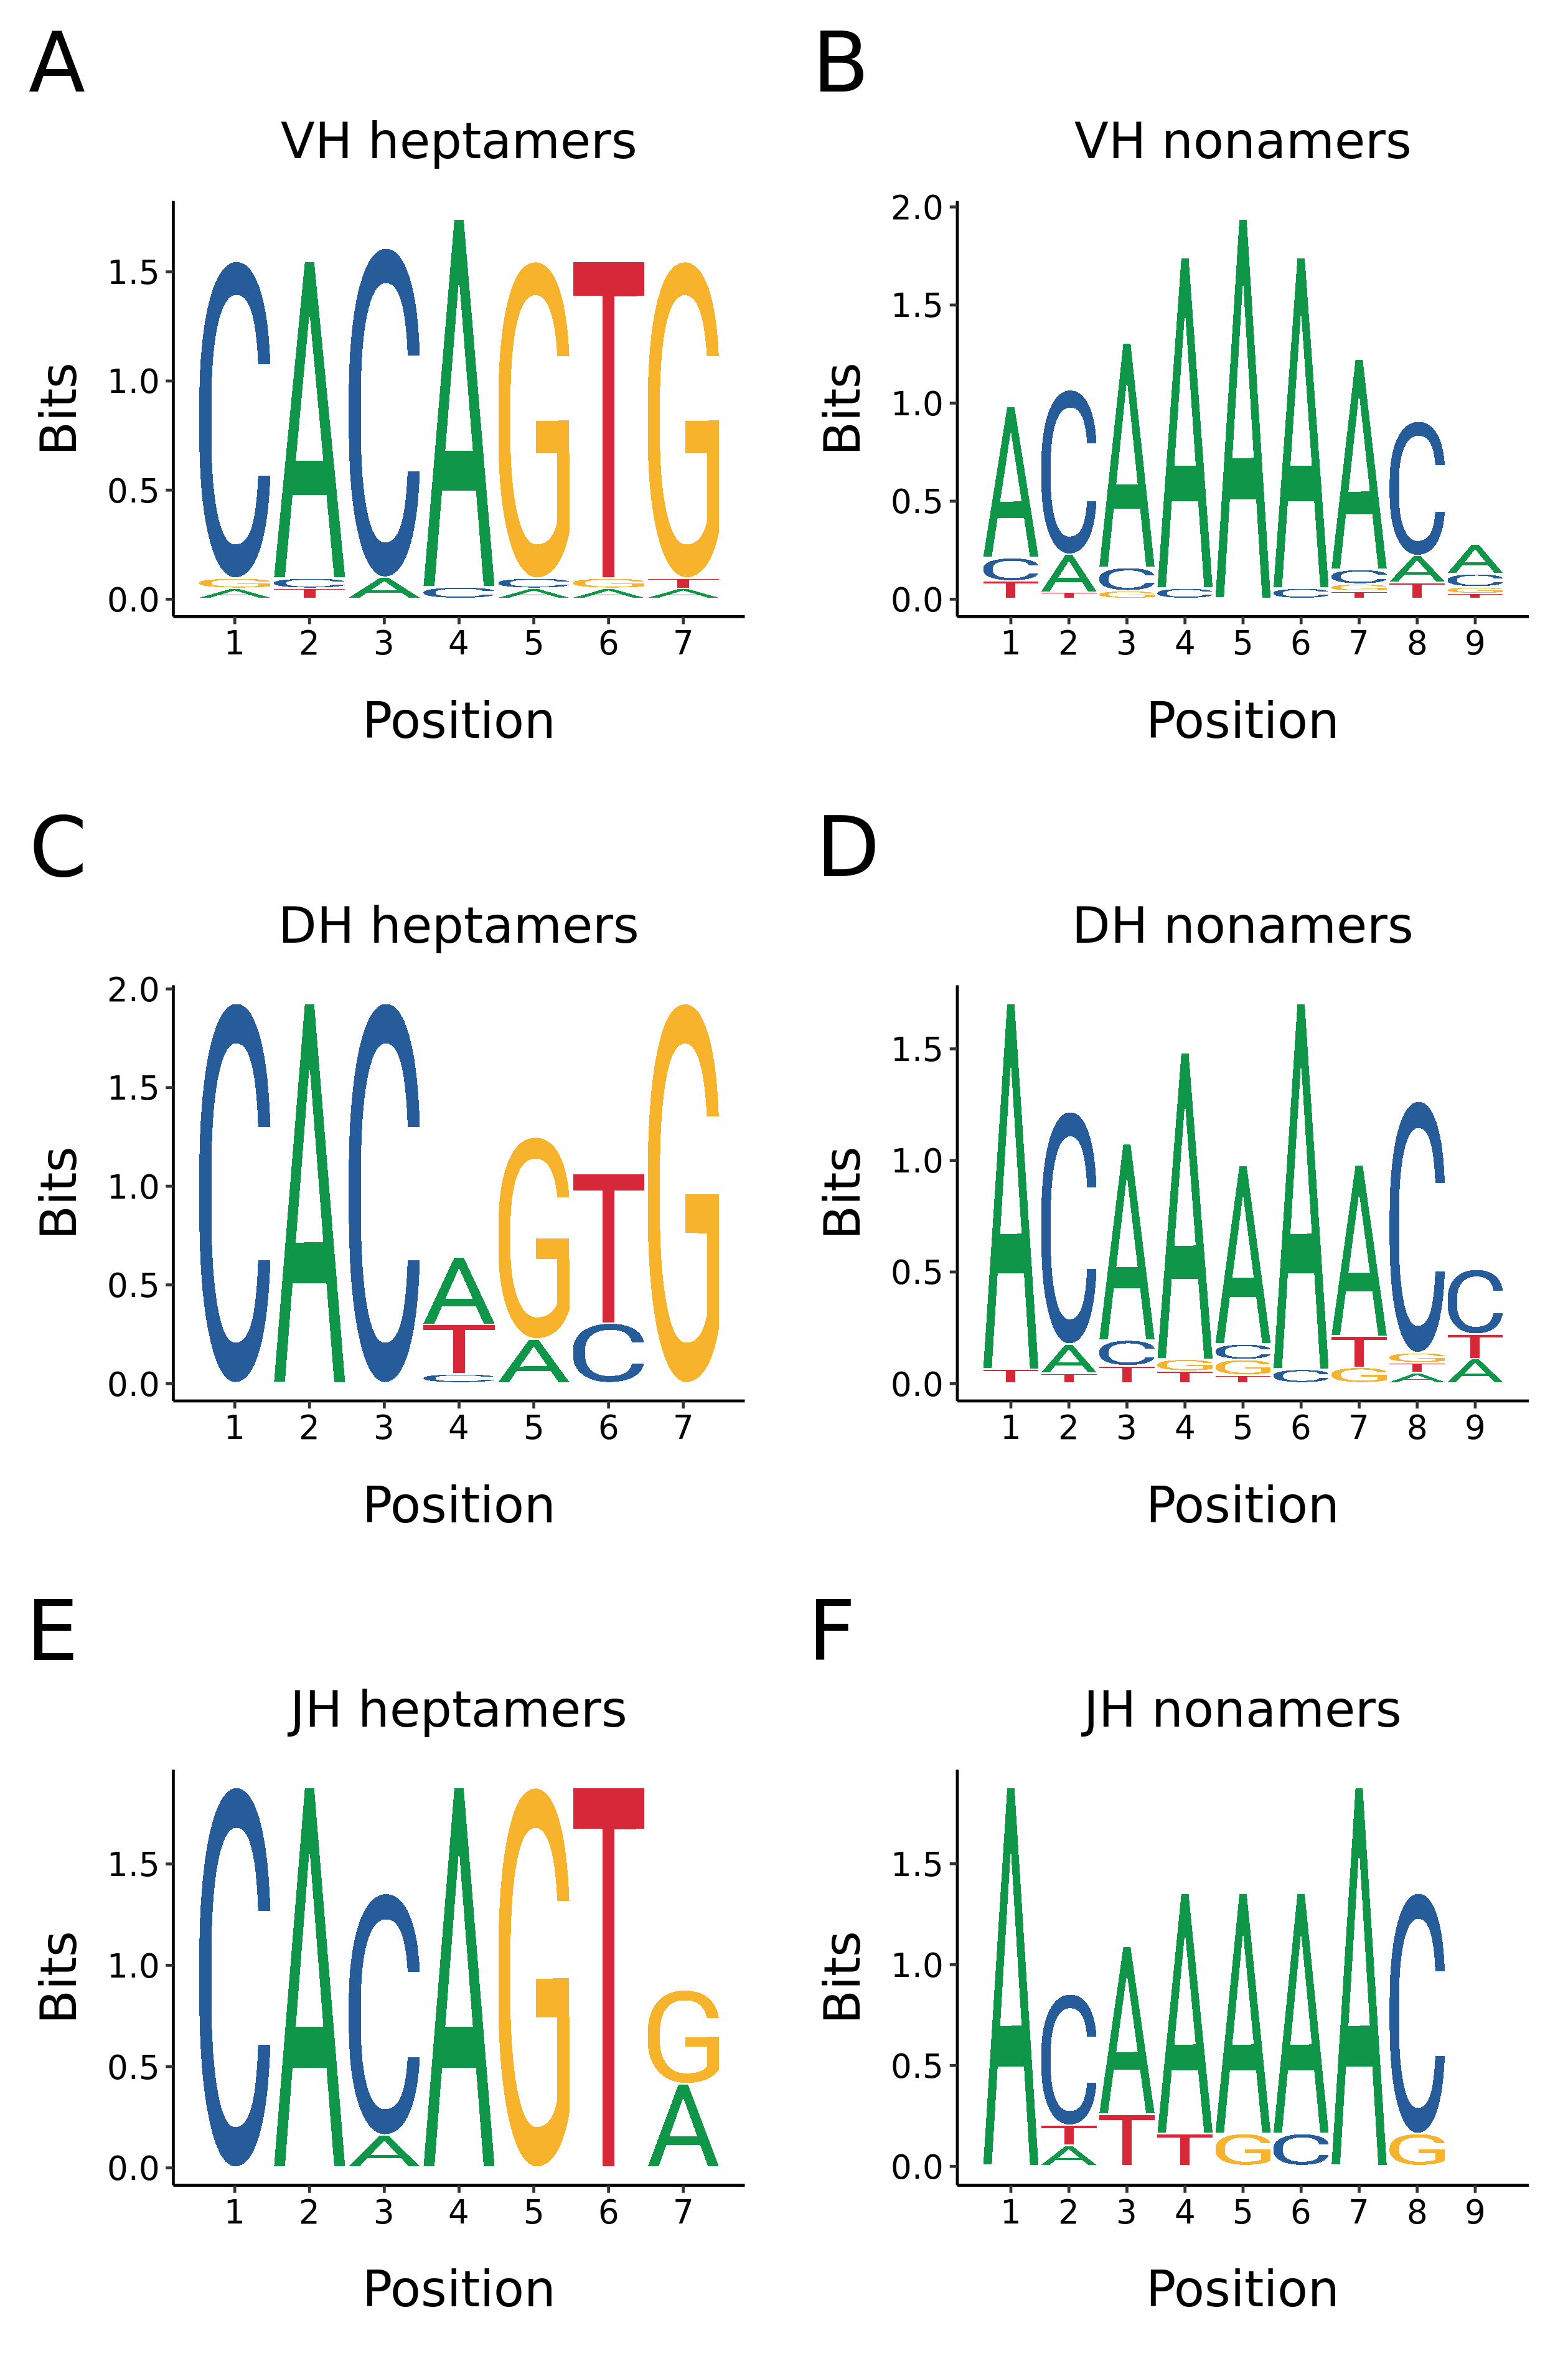
\includegraphics[width=0.9\textwidth]{_Figures/png/nfu-rss-seqlogo-sep}
	\Caption{\Nfu recombination signal sequences by segment type}{Sequence composition of conserved heptamer (A,C,E) and nonamer (B,D,F) sequences from \Nfu heavy-chain RSSs associated with \vh (A,B), \dh (C,D) or \jh (E,F) gene segments.}
	\label{fig:nfu-rss-seqlogo-sep}
\end{figure}

	\begin{figure}
	\centering
	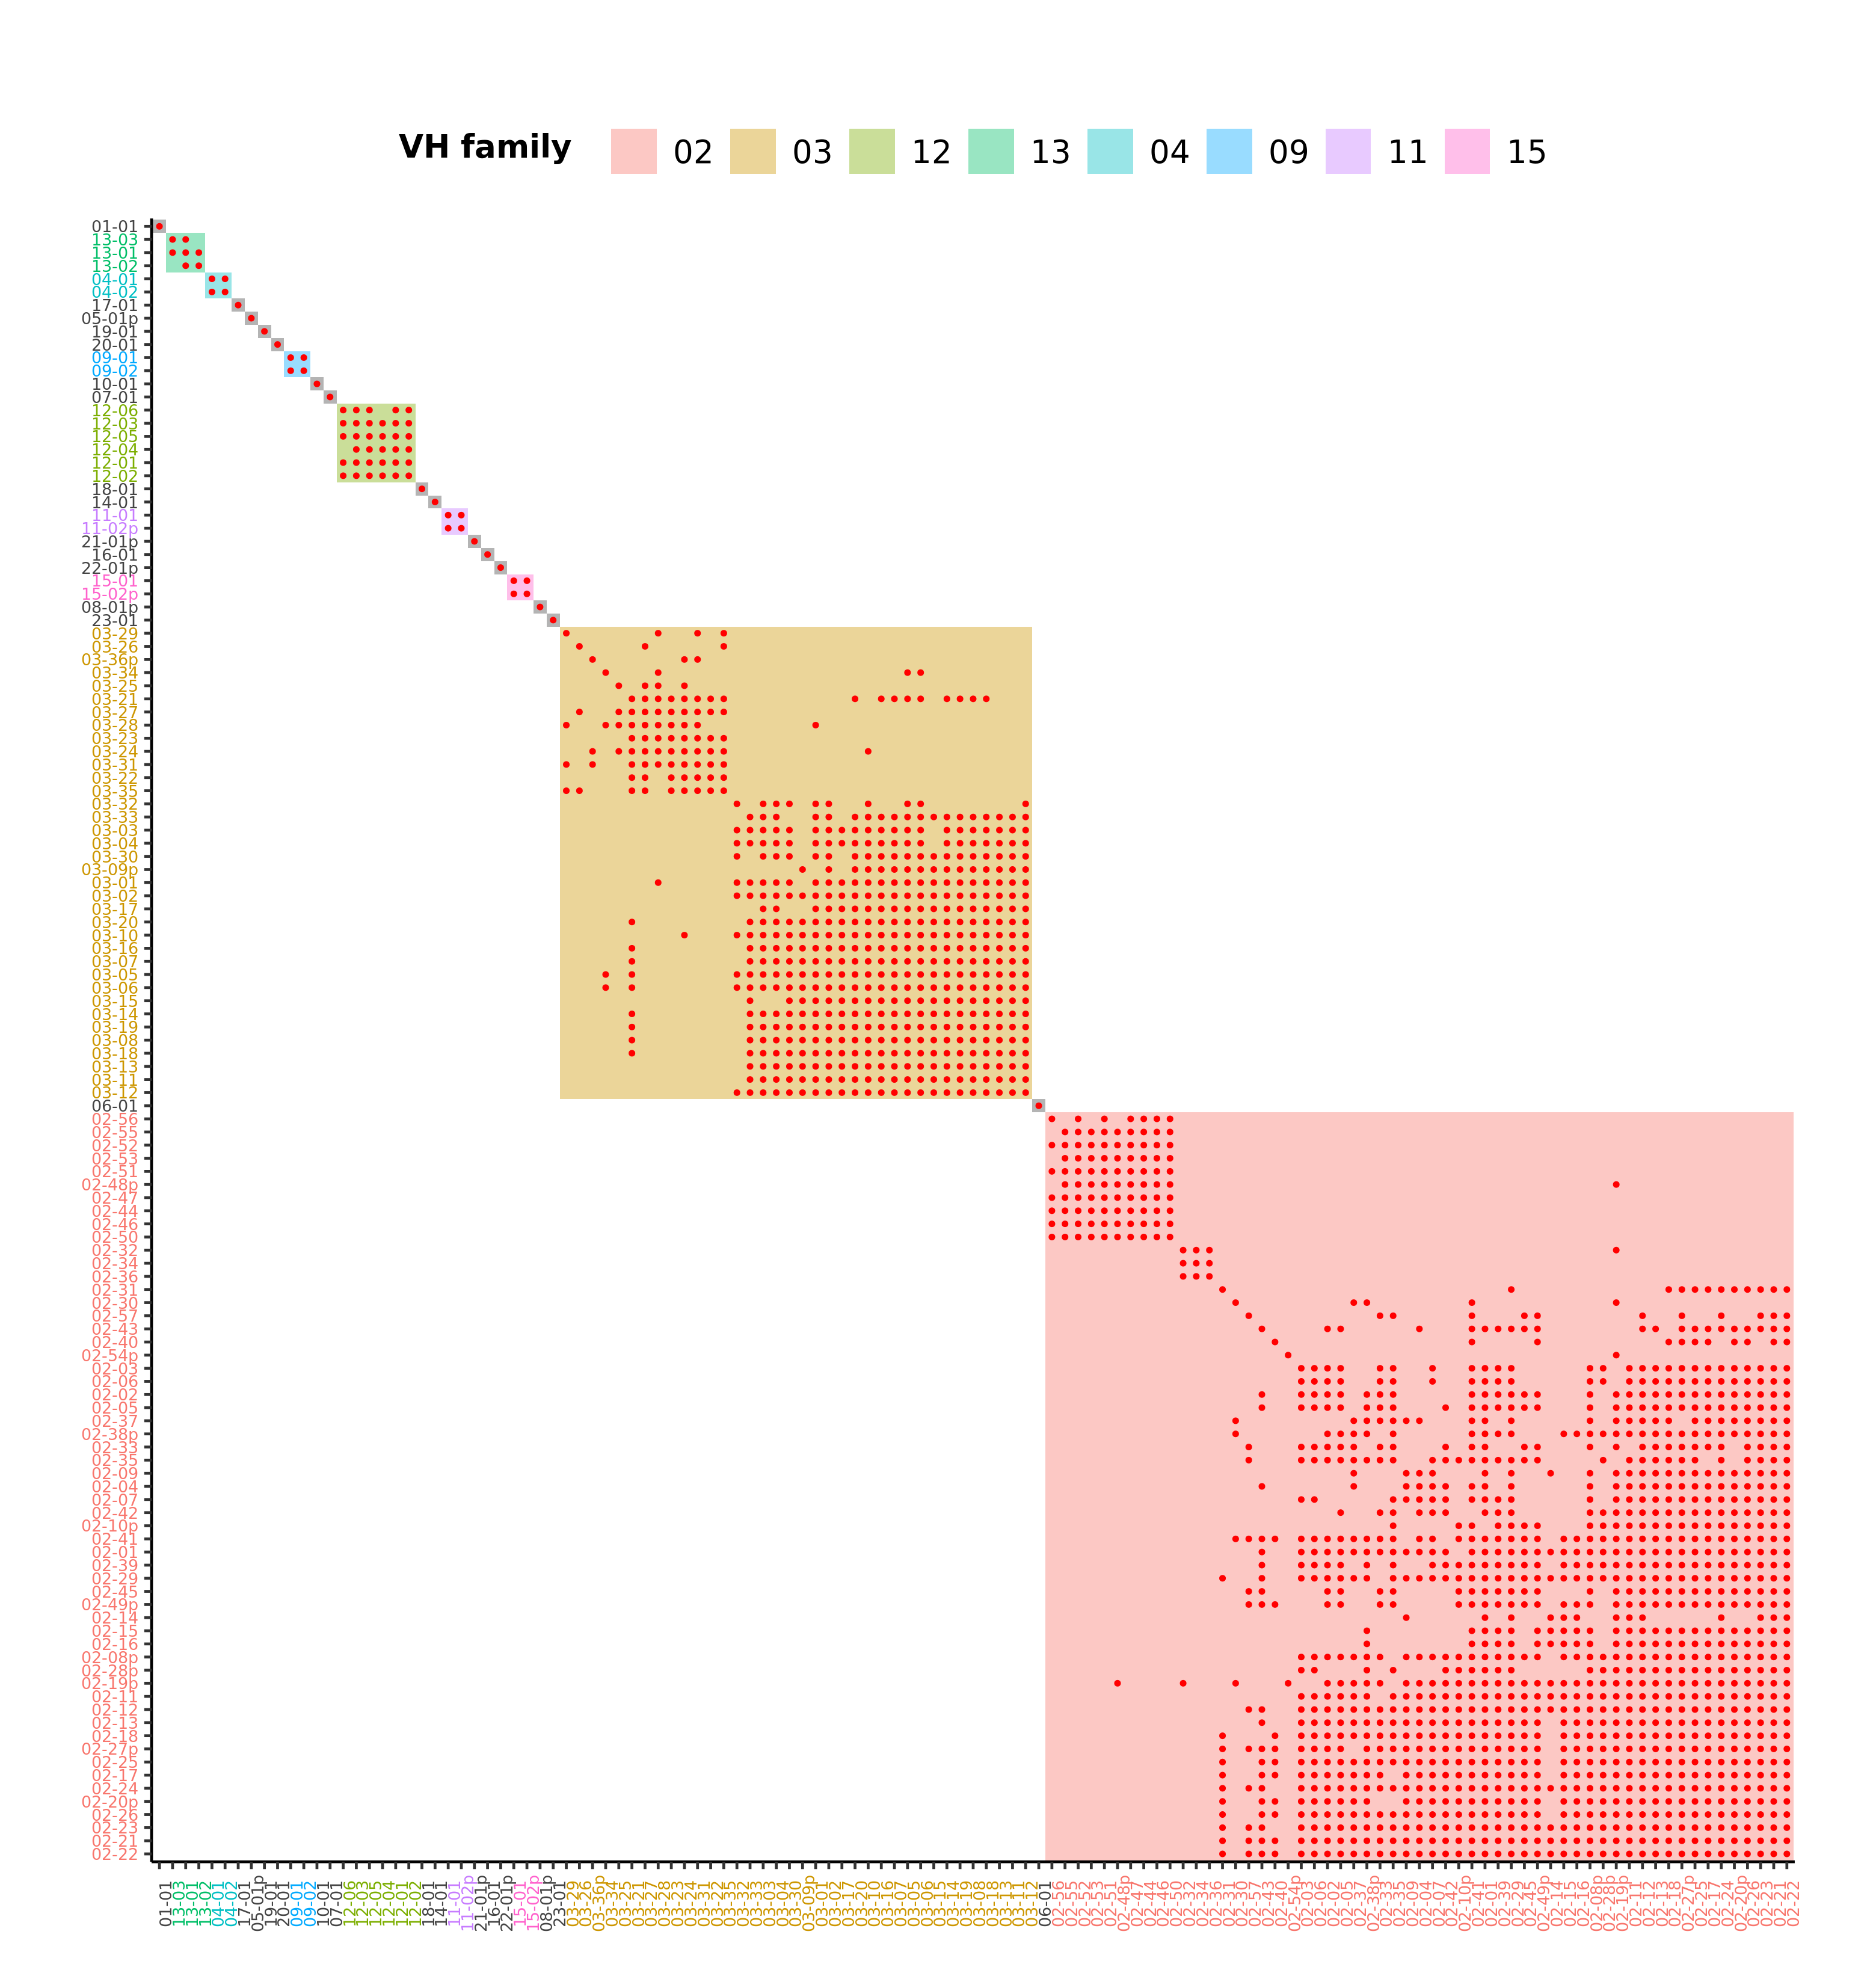
\includegraphics[width=\textwidth]{_Figures/png/xma-vh-families-map}
	\Caption{Heatmap of \vh families in the \Xma \igh{} locus}{Heatmap of family relationships among \Xma \vh segments, with coloured shading indicating families and red dots indicating pairwise nucleotide sequence identity of at least 80\%. \vh families containing multiple segments are uniquely coloured, while single-segment families are in grey.}
	\label{fig:xma-vh-families-map}
	\end{figure}

	\begin{figure}
	\centering
	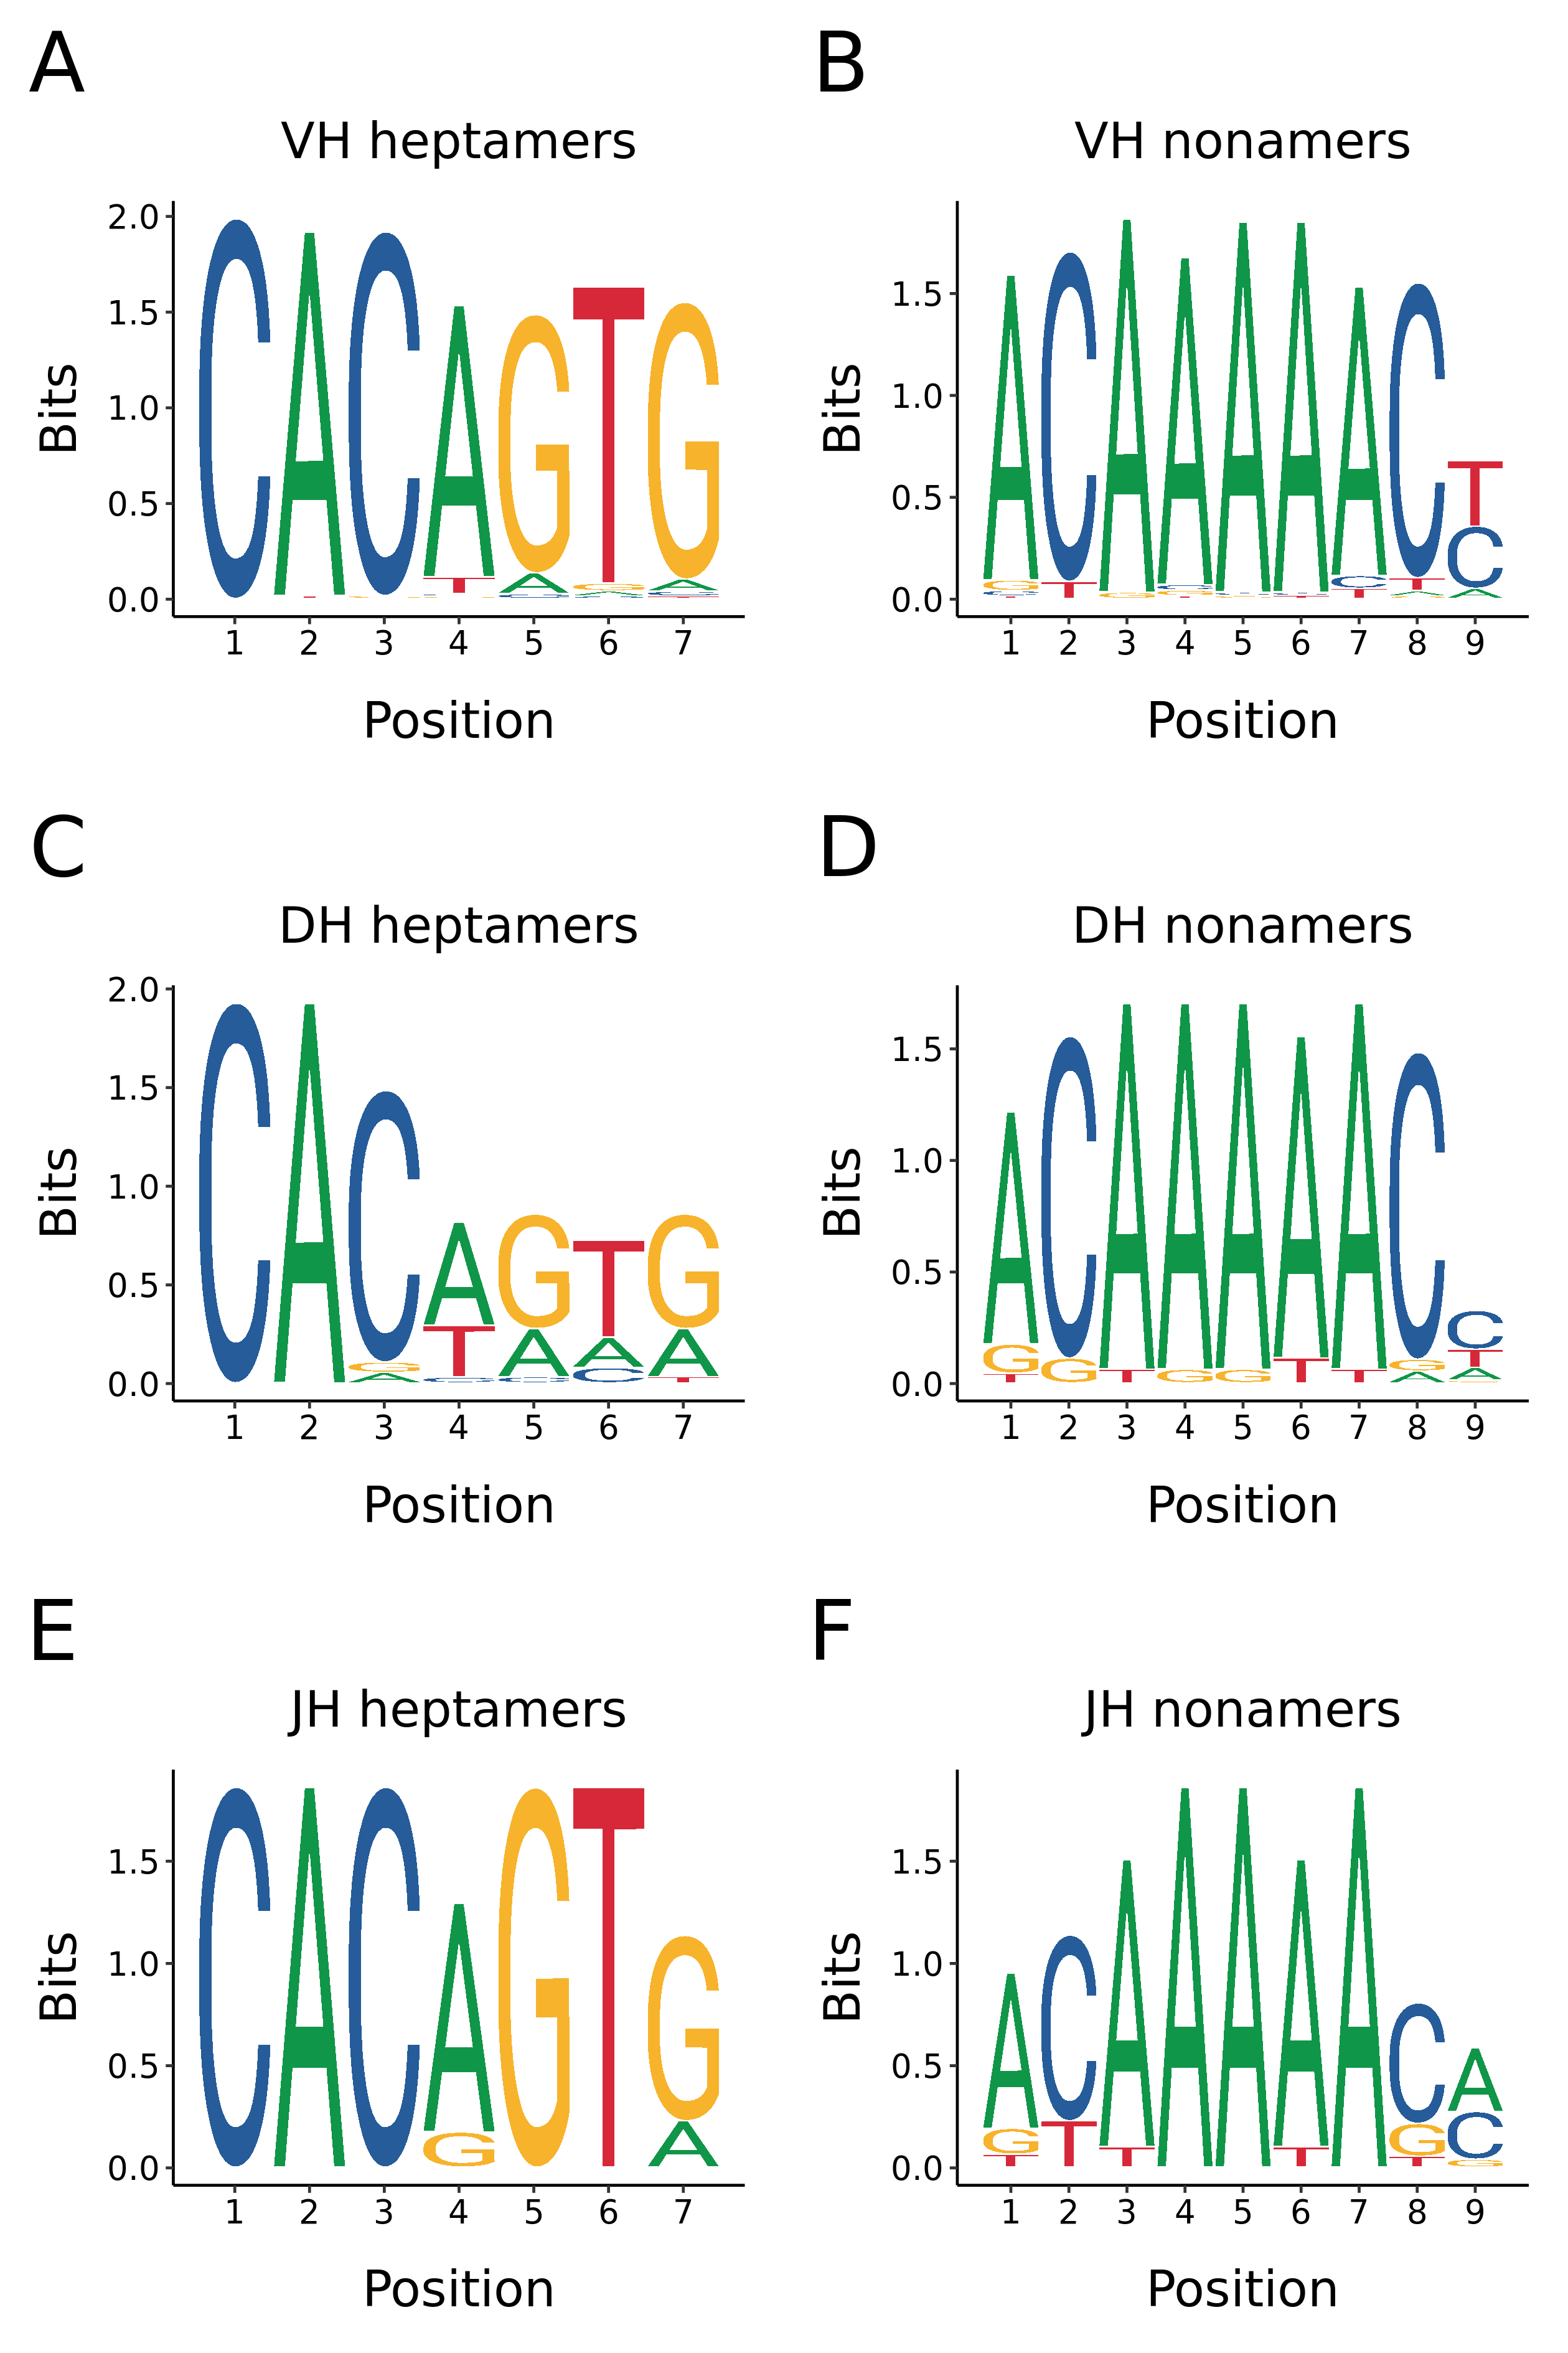
\includegraphics[width=0.9\textwidth]{_Figures/png/xma-new-rss-seqlogo-sep}
	\Caption{\Xma recombination signal sequences by segment type}{Sequence composition of conserved heptamer (A,C,E) and nonamer (B,D,F) sequences from \Xma heavy-chain RSSs associated with \vh (A,B), \dh (C,D) or \jh (E,F) gene segments.}
	\label{fig:xma-rss-seqlogo-sep}
	\end{figure}
	
	\begin{figure}
\centering
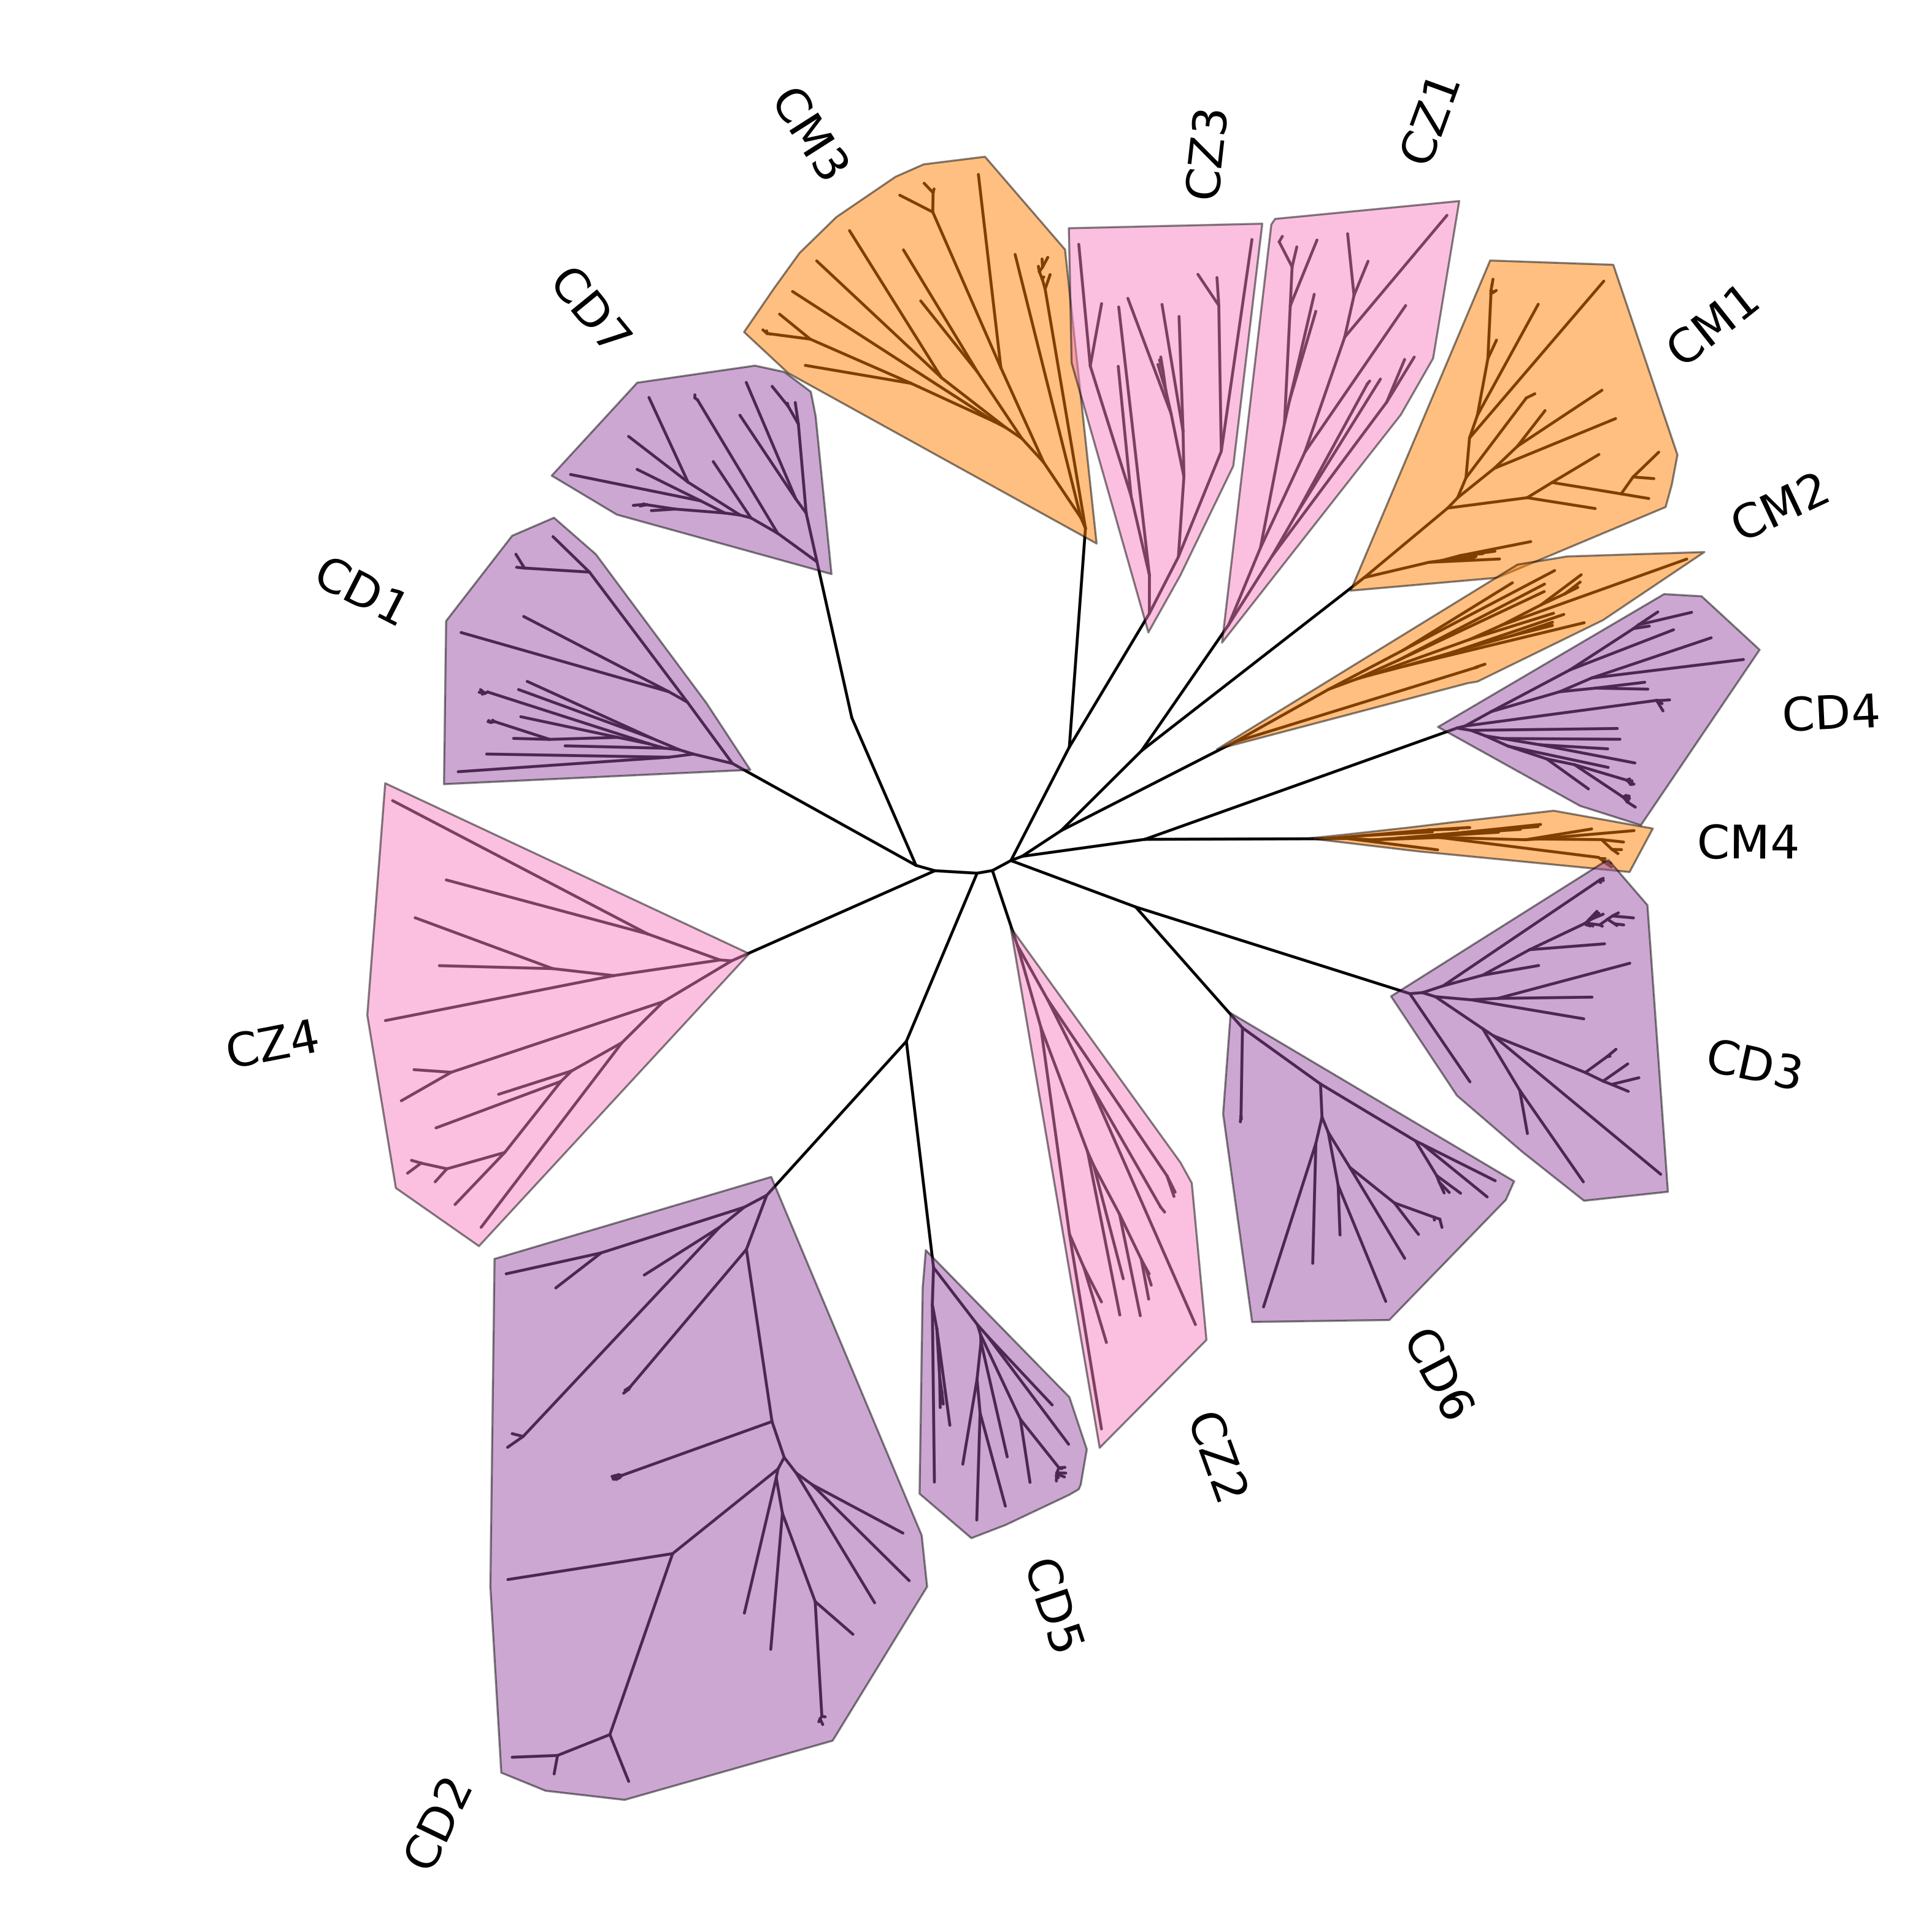
\includegraphics[width=0.9\textwidth]{_Figures/png/ch-tree-all}
\Caption{Constant-region \ch exons in the Atherinomorpha}{Unrooted phylogram of \ch exons from thirteen fish species from the Atherinomorpha (\Cref{tab:cyprinodontiform-genomes}), constructed using \program{PRANK} and \program{RAxML}. Each exon type is clustered separately in the tree topology, indicating that the types of the identified exons have all been correctly annotated.}
\label{fig:ch-tree-all}
\end{figure}

\begin{figure}
	\centering
	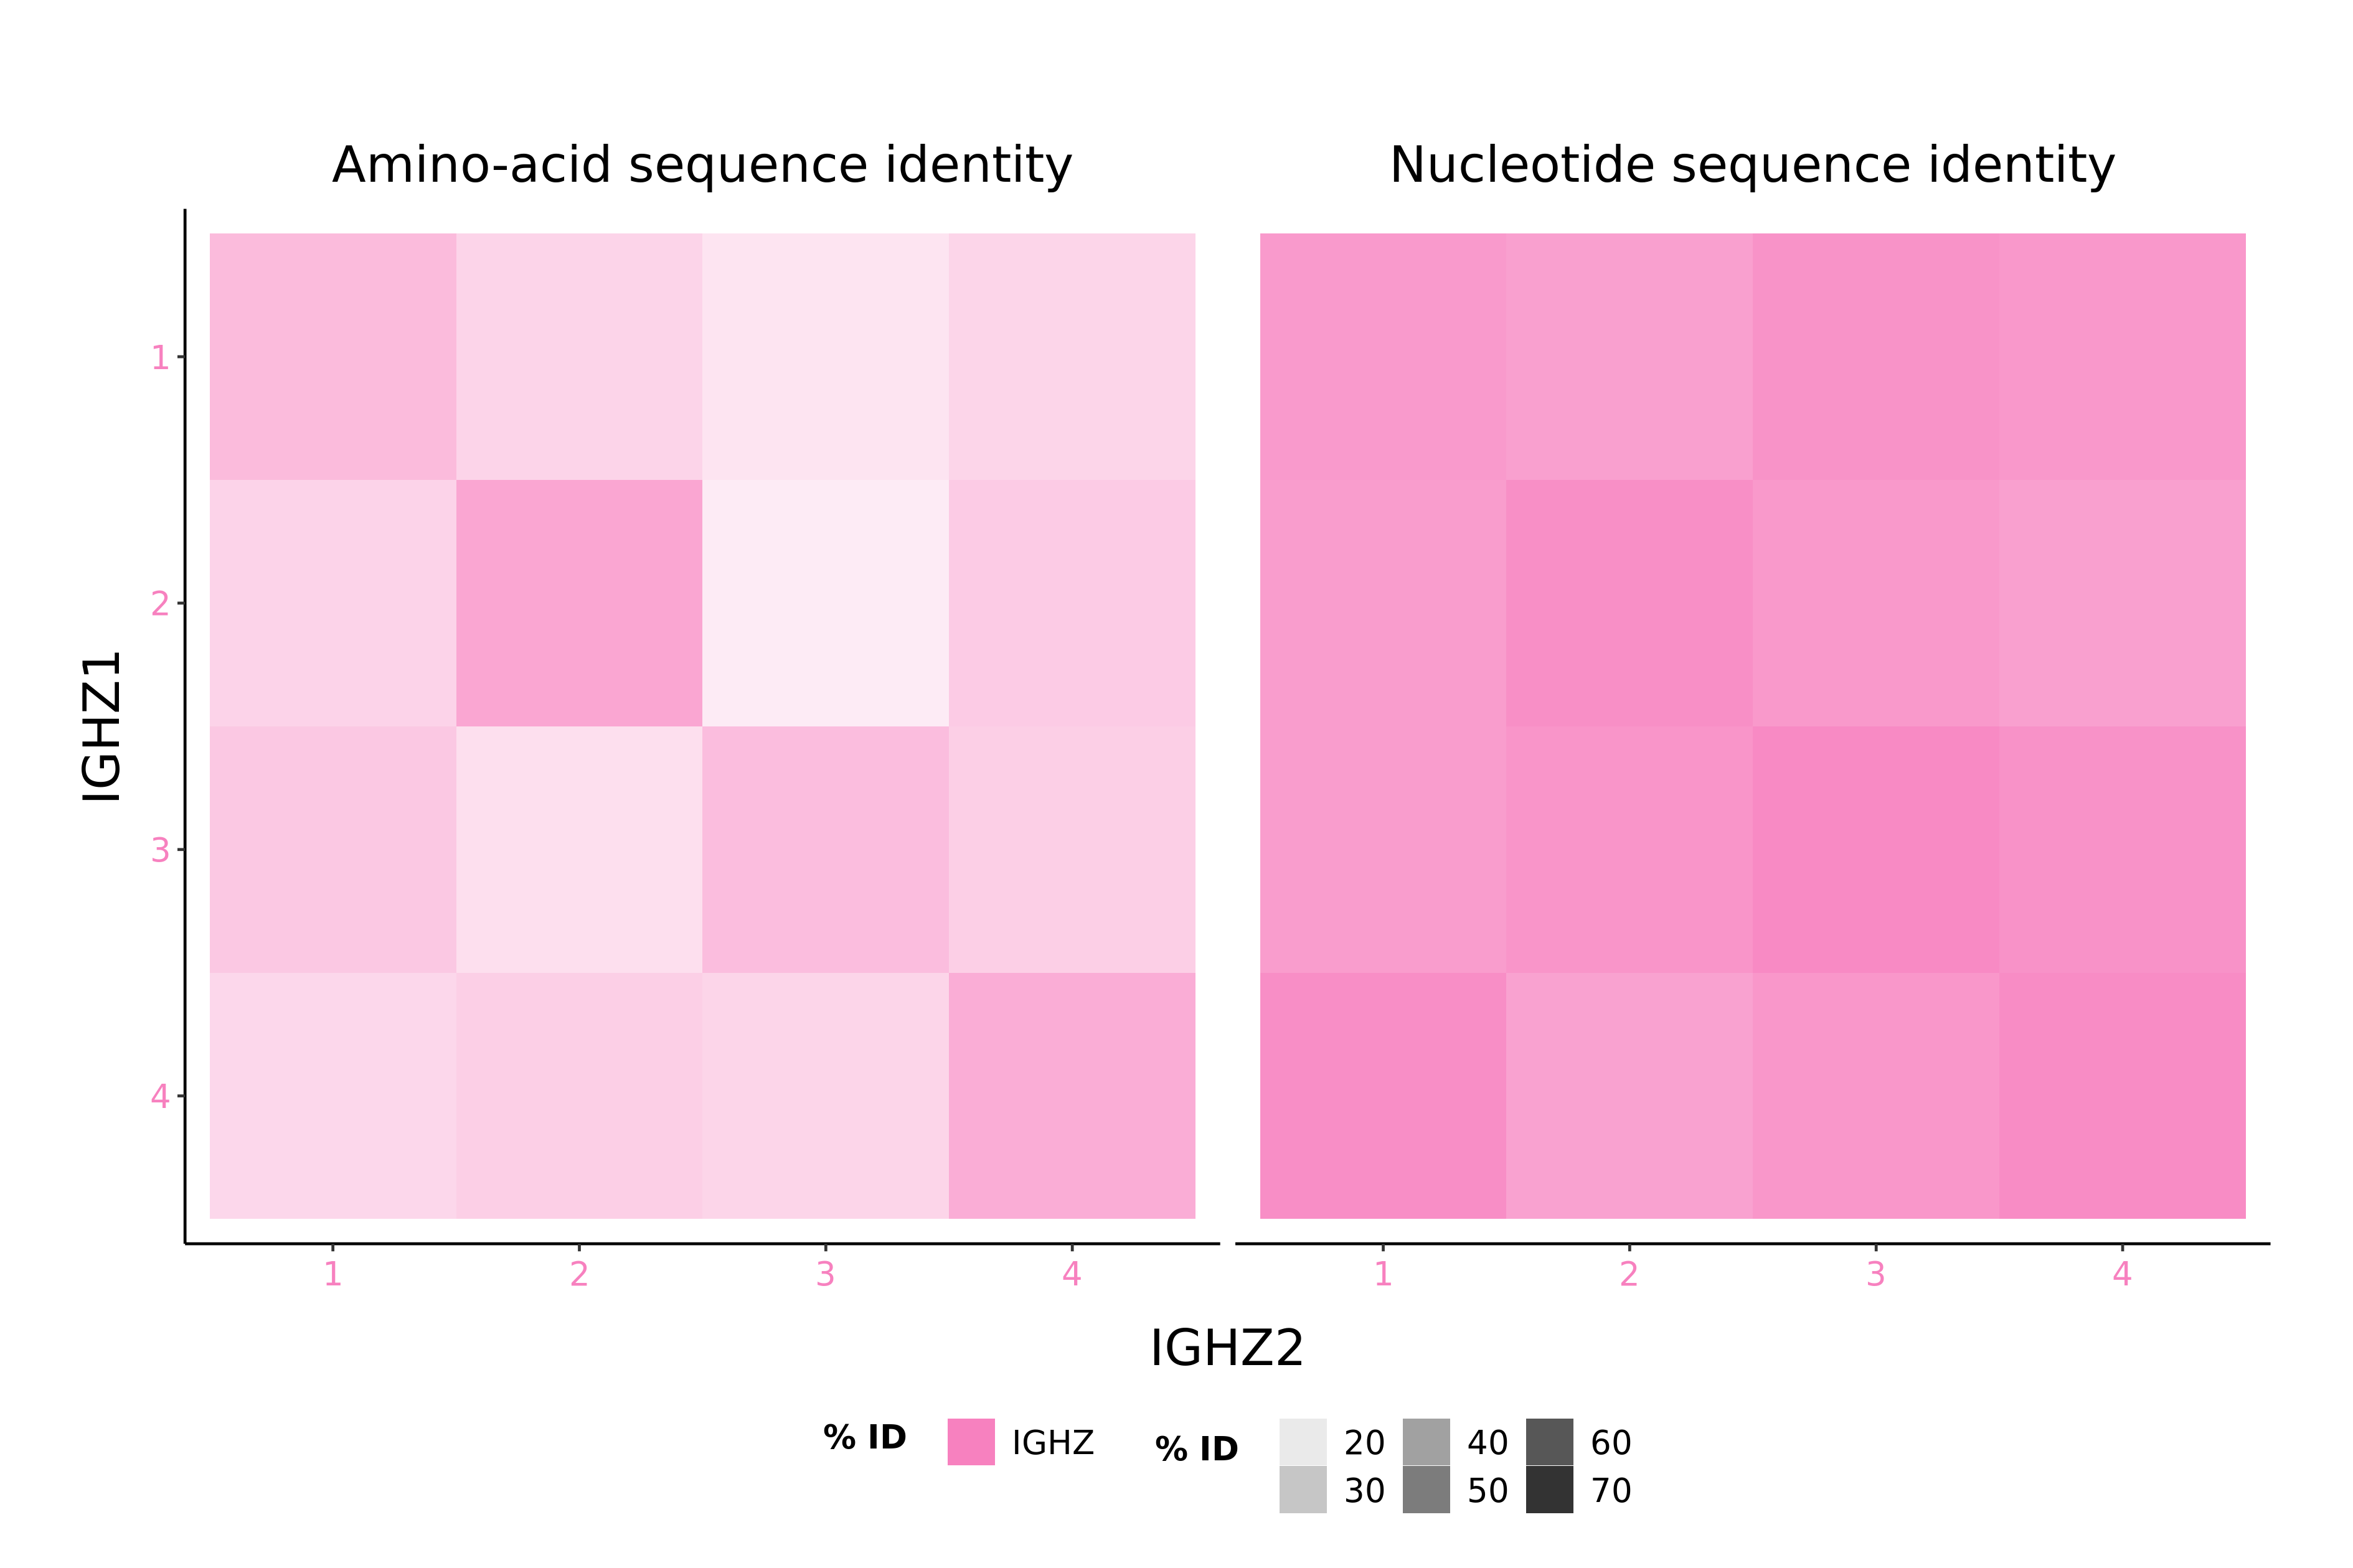
\includegraphics[width=0.8\textwidth]{_Figures/png/xma-new-cz-aln}
	\Caption{Sequence similarity between \igh{Z} constant-regions in \Xma}{Heatmap of percentage sequence identity between amino-acid (right) and nucleotide (left) sequences of \cz{} exons from the two \Xma \igh{Z} constant regions, calculated using pairwise Needleman-Wunsch global alignments.}
	\label{fig:xma-cz-aln}
\end{figure}
	
% 4 - IGSEQ CHAPTER

\begin{figure}
\centering
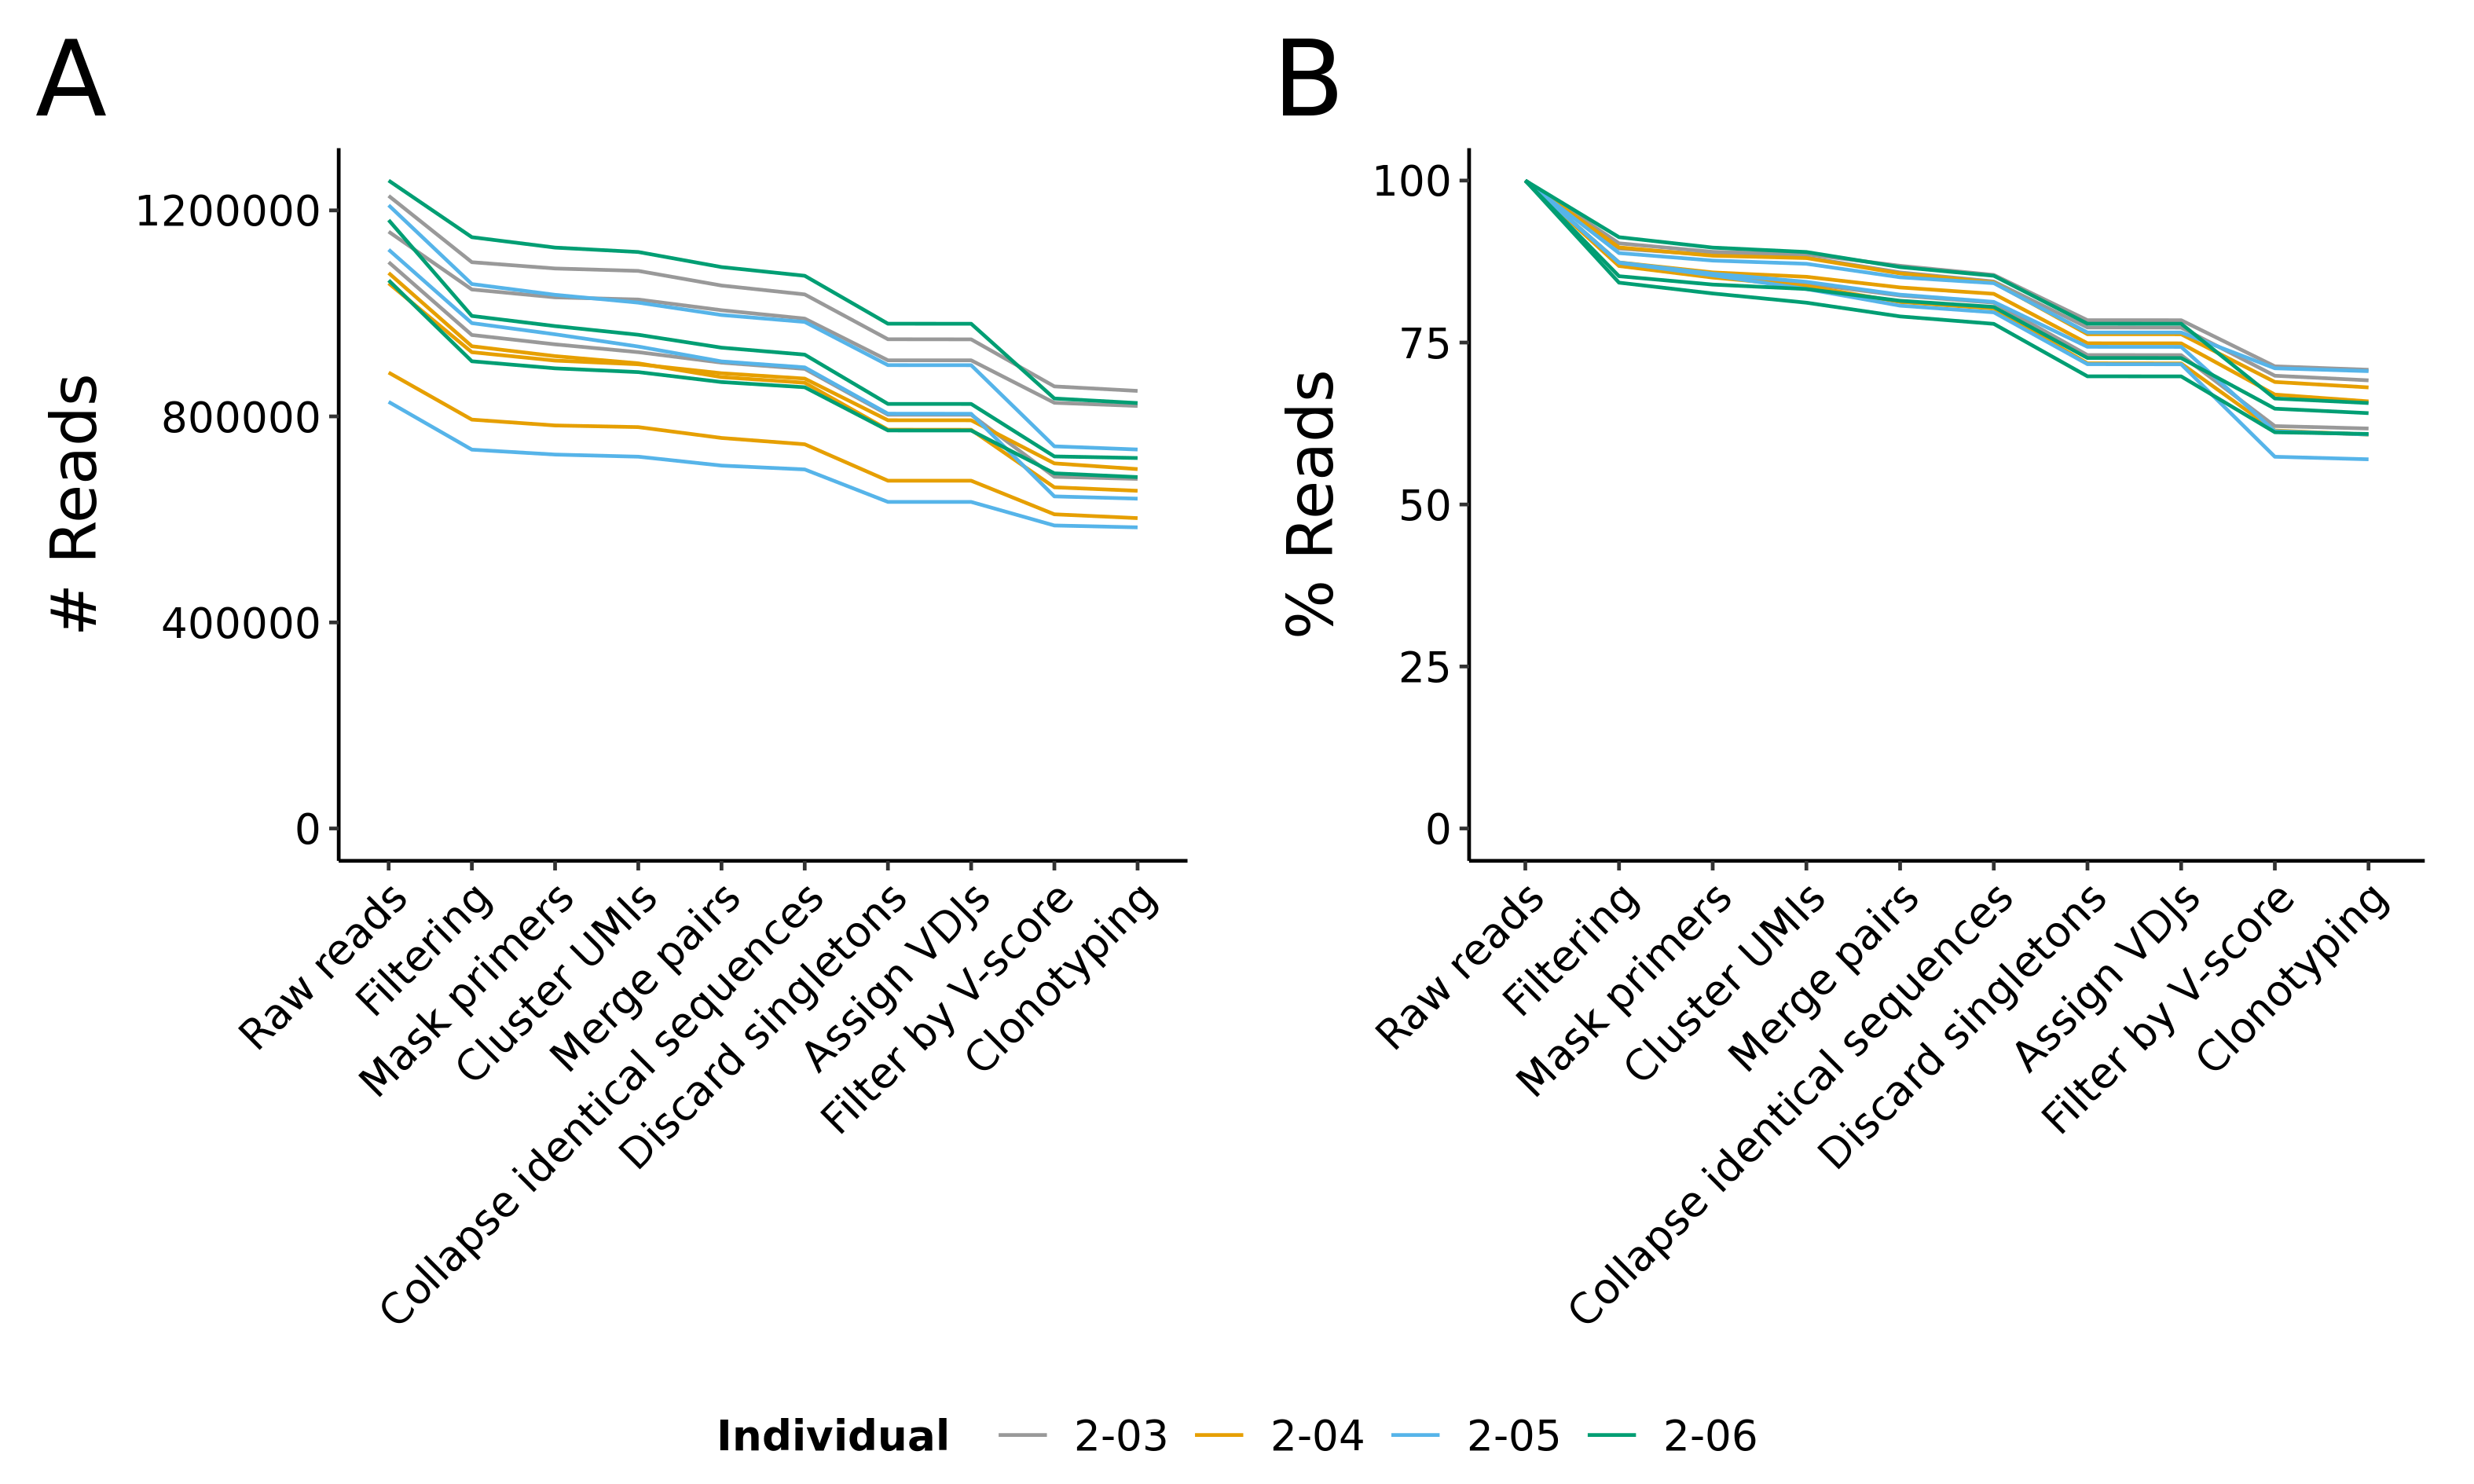
\includegraphics[width = 0.9\textwidth]{_Figures/png/pilot-read-survival-all.png}
\begin{subfigure}{0em}
\phantomsubcaption{}
\label{fig:igseq-pilot-read-survival-all-a}
\end{subfigure}
\begin{subfigure}{0em}
\phantomsubcaption{}
\label{fig:igseq-pilot-read-survival-all-b}
\end{subfigure}
\Caption{Read survival during complete pre-processing of the \igseq pilot dataset}{Line graphs of absolute (A) and relative (B) read survival during pre-processing of the \igseq pilot dataset, up to and including clonotyping.}
\label{fig:igseq-pilot-read-survival-all}
\end{figure}

\begin{figure}
\centering
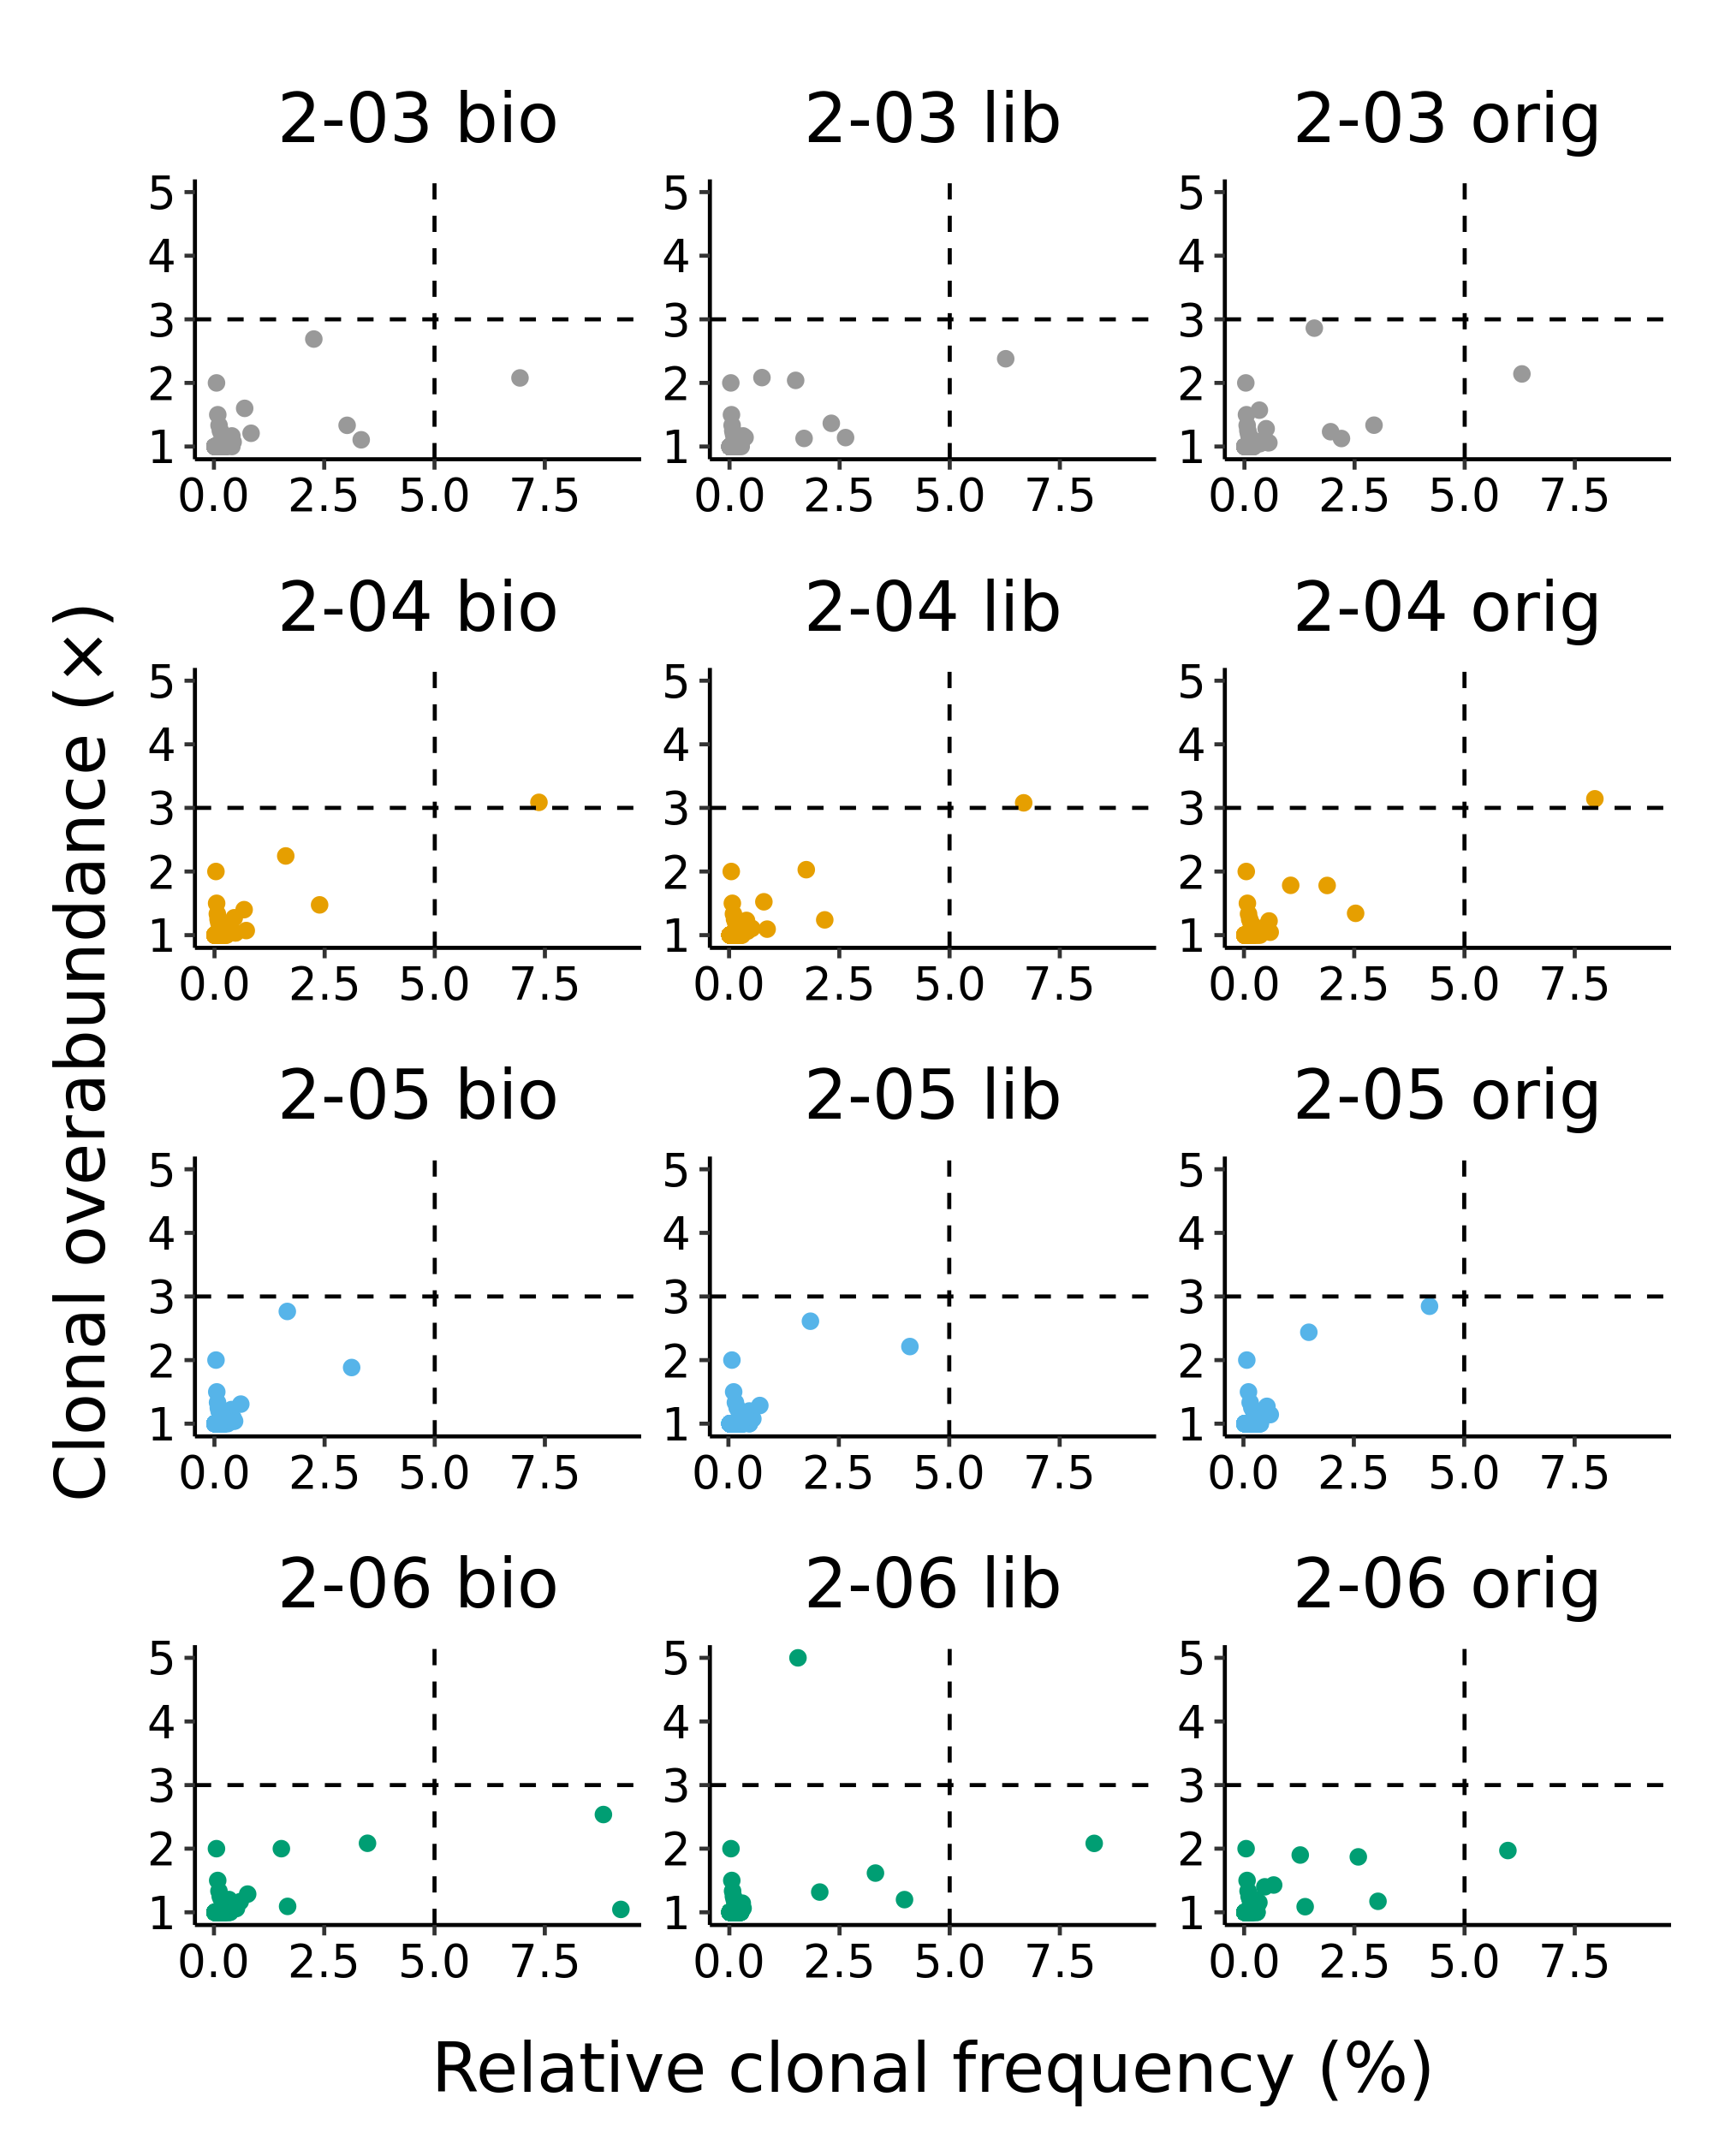
\includegraphics[width=0.8\textwidth]{_Figures/png/pilot-clones-expansions-rep}
\Caption{Clonal expansions in \Nfu pilot replicates}{Scatter plots of clonal abundance for each replicate in the \igseq pilot dataset, measured in terms of the proportion of unique sequences in the repertoire ($x$-axis) and the abundance relative to the next-largest clone ($y$-axis). Thresholds for identifying clonal expansions (5\,\% and 3-fold for the $x$- and $y$-axis, respectively) suggested by Rosenfeld \textit{et al.} \parencite{rosenfeld2018clonesize}.}
\label{fig:igseq-pilot-clones-expansions-rep}
\end{figure}

\begin{figure}
\centering
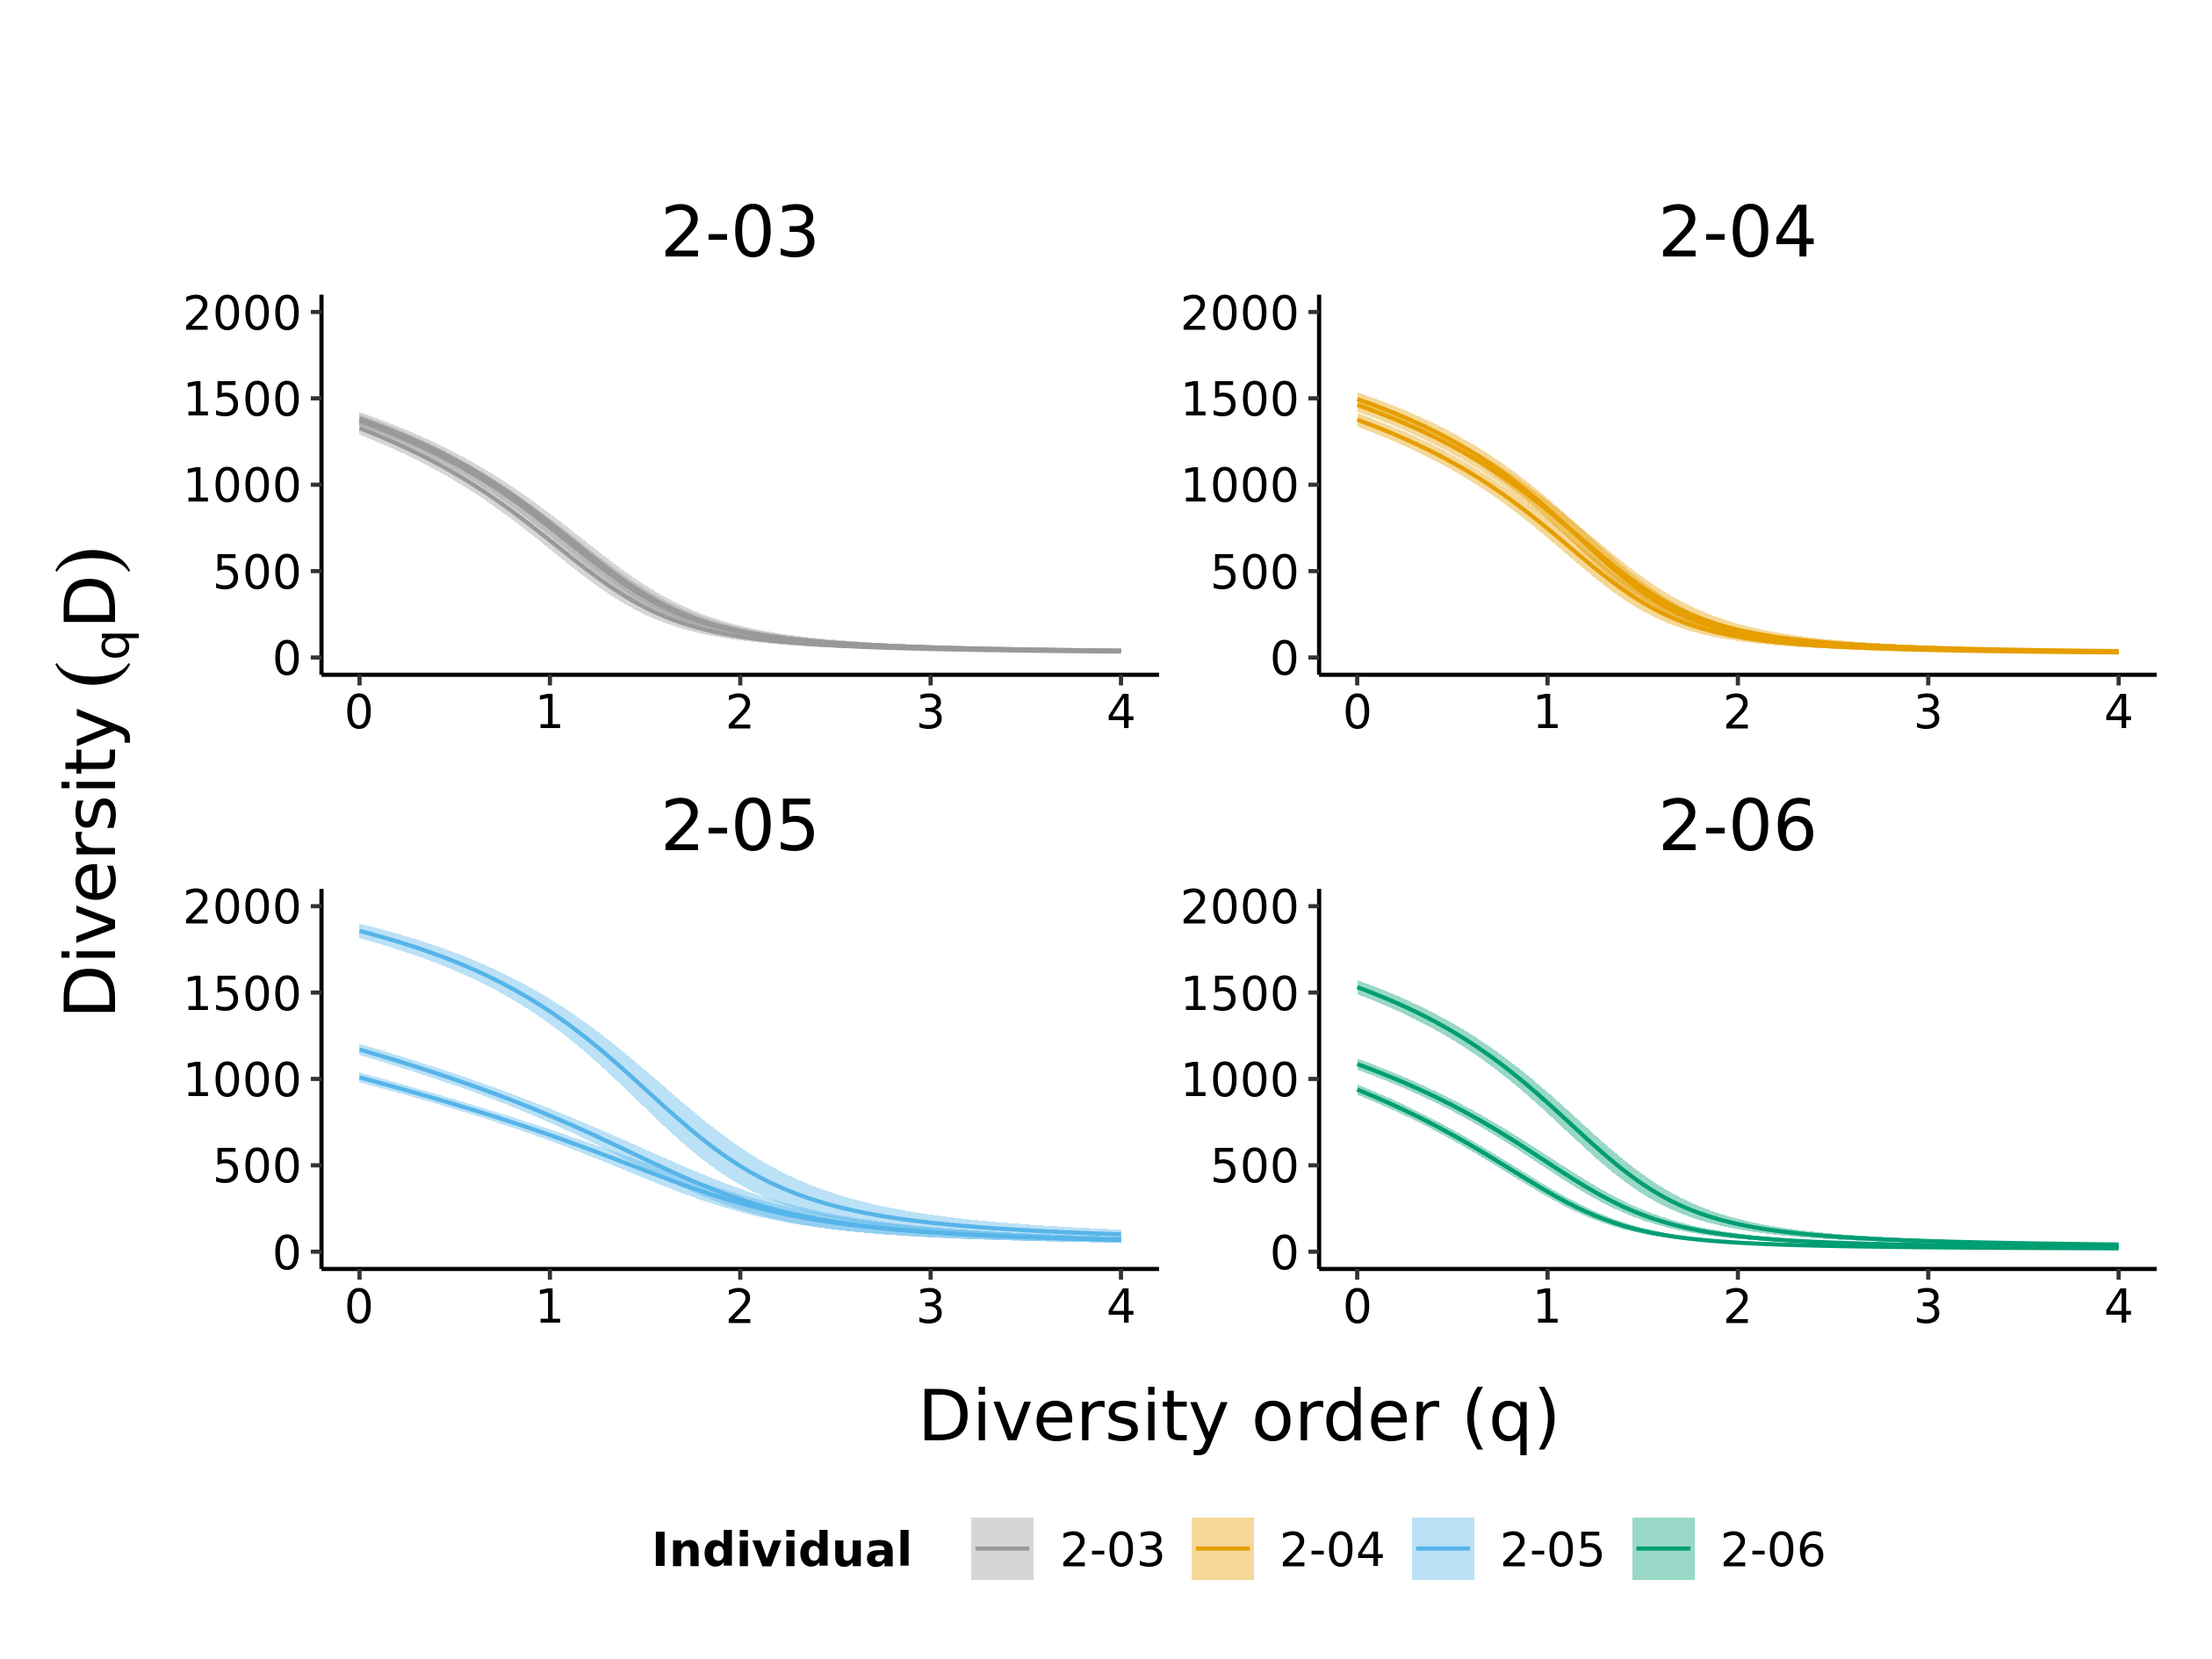
\includegraphics[width = 0.8\textwidth]{_Figures/png/pilot-clone-diversity-solo-spectra}
\Caption{Per-replicate clonal-diversity spectra for the \igseq pilot dataset}{Hill diversity spectra of clone sizes (as measured by number of unique sequences per clone) for each replicate in the \igseq pilot dataset, grouped by source individual.}
\label{fig:igseq-pilot-clone-diversity-solo-spectra}
\end{figure}

\begin{figure}
\centering
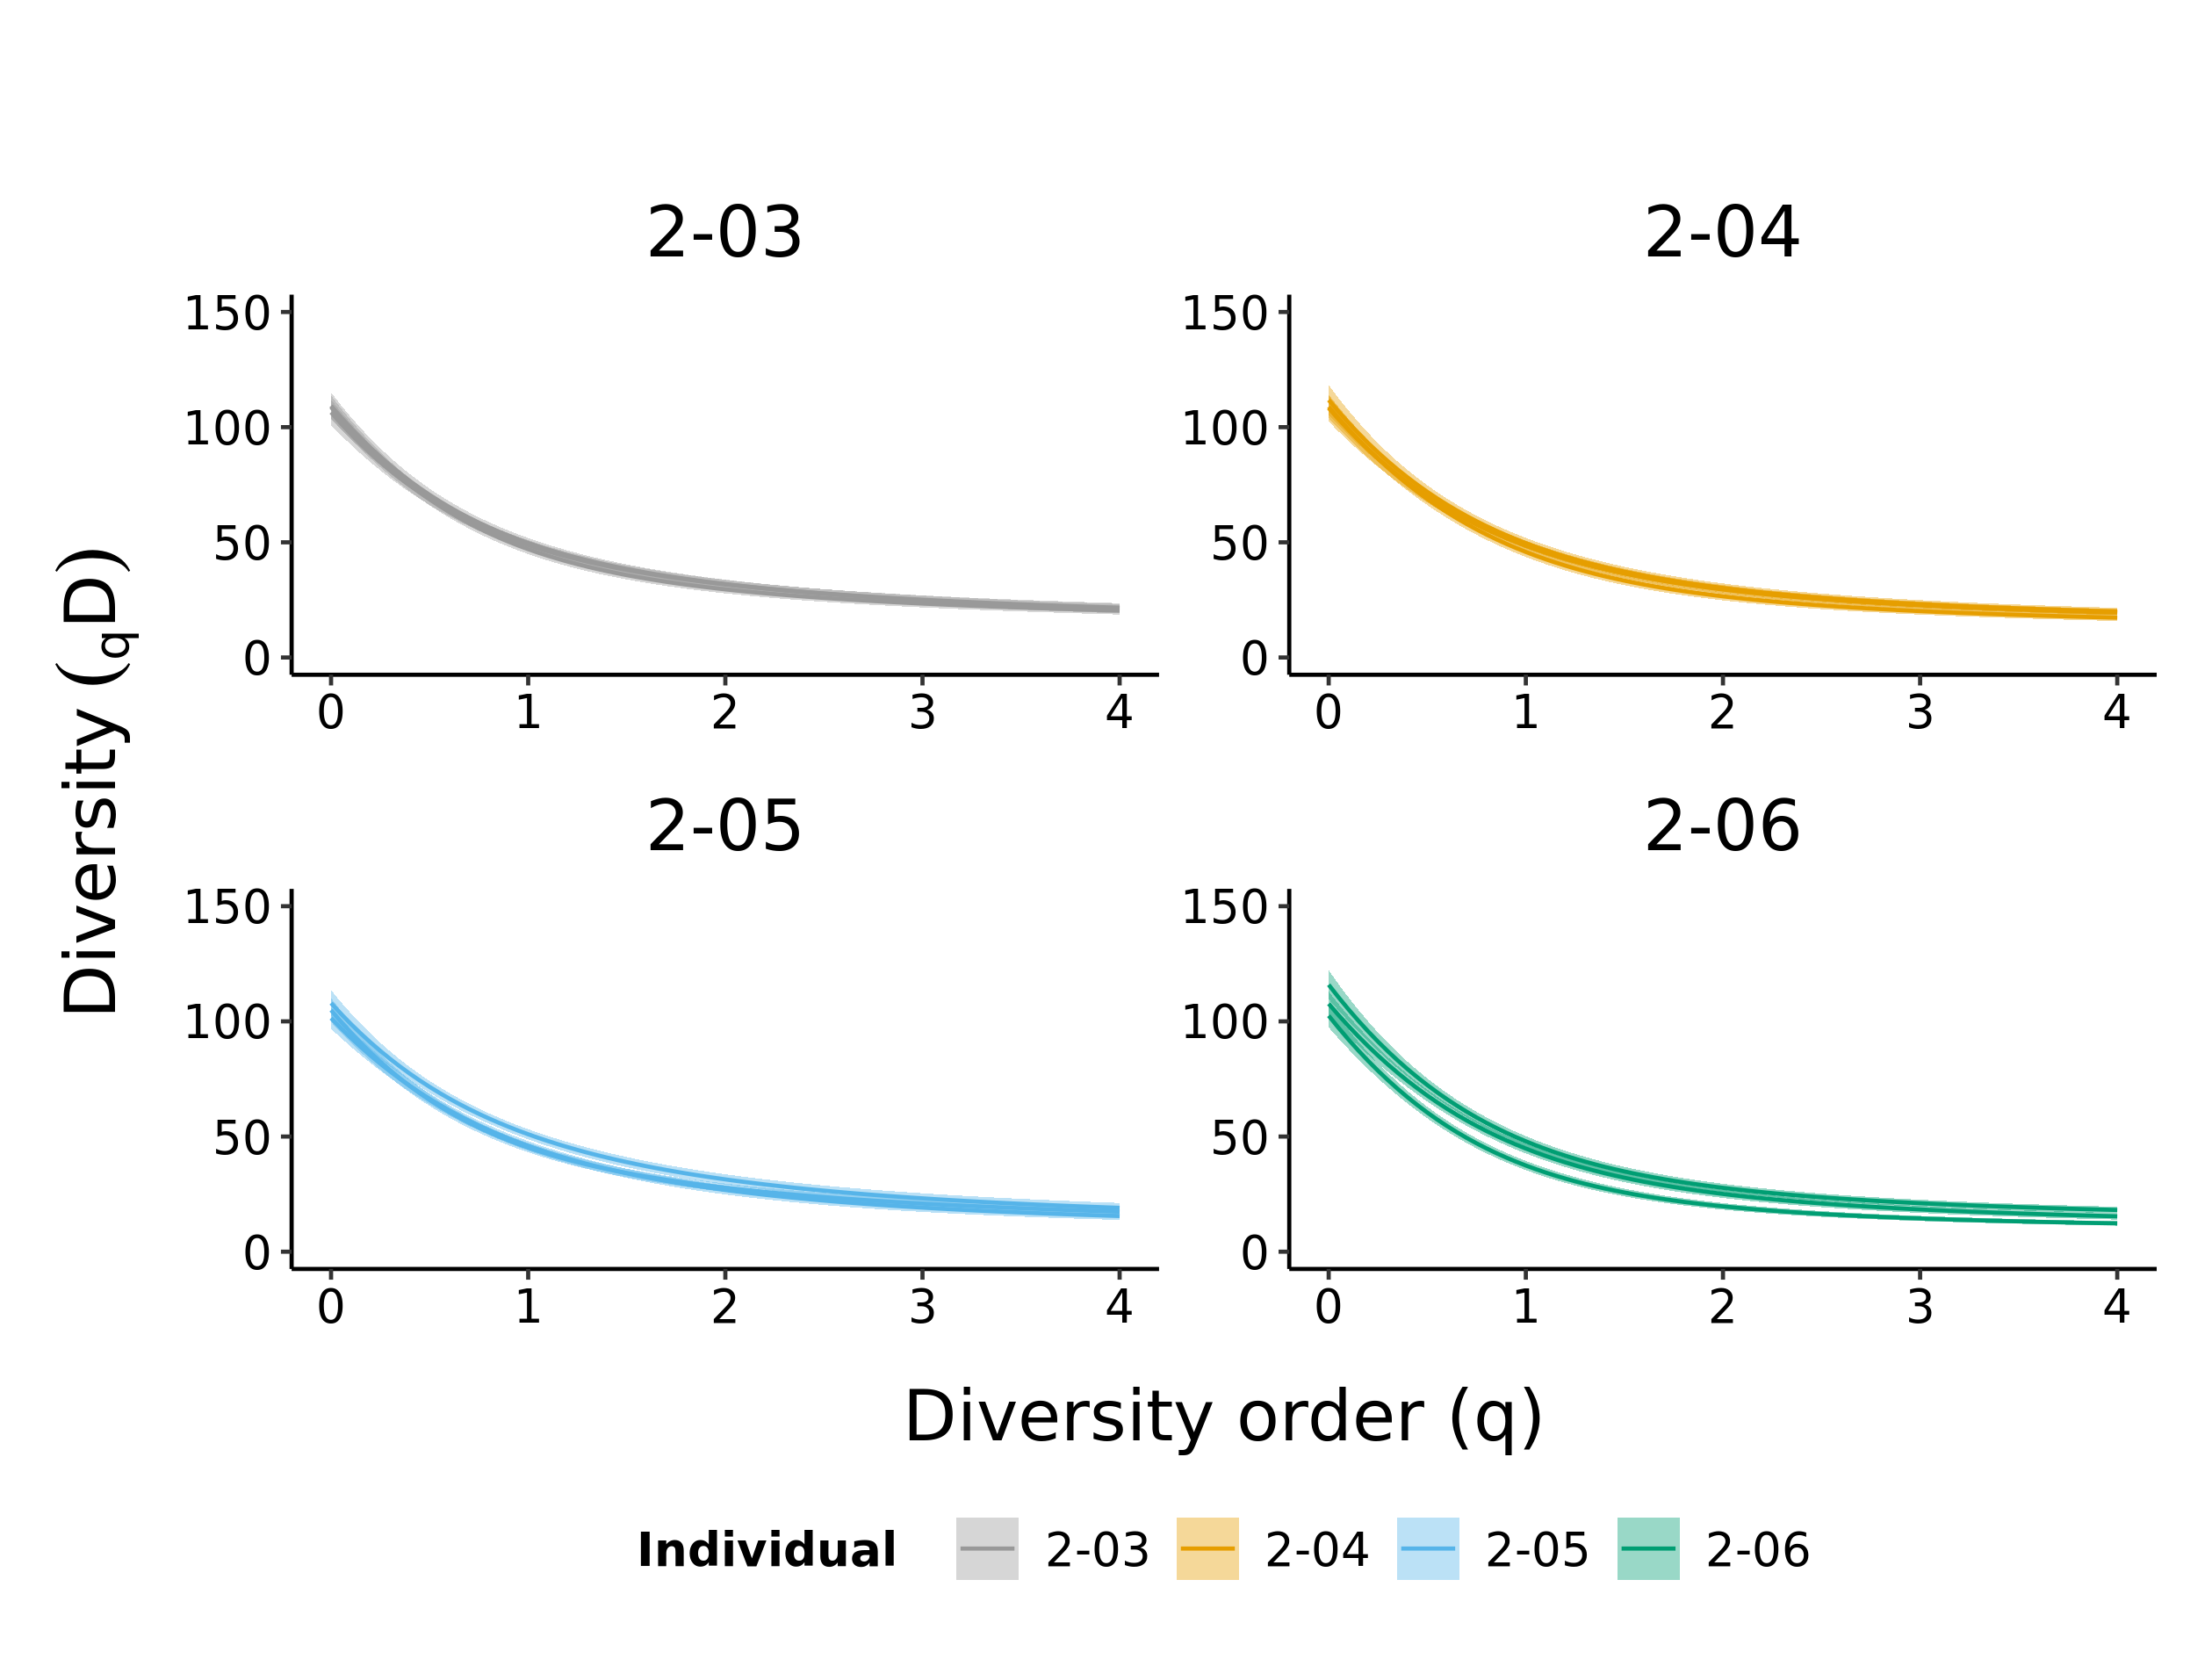
\includegraphics[width = 0.8\textwidth]{_Figures/png/pilot-vj-diversity-solo-spectra}
\Caption{Per-replicate VJ-diversity spectra for the \igseq pilot dataset}{Hill diversity spectra of VJ usage (as measured by number of unique sequences per V/J combination) for each replicate in the \igseq pilot dataset, grouped by source individual.}
\label{fig:igseq-pilot-vj-diversity-solo-spectra}
\end{figure}

\begin{figure}
\centering
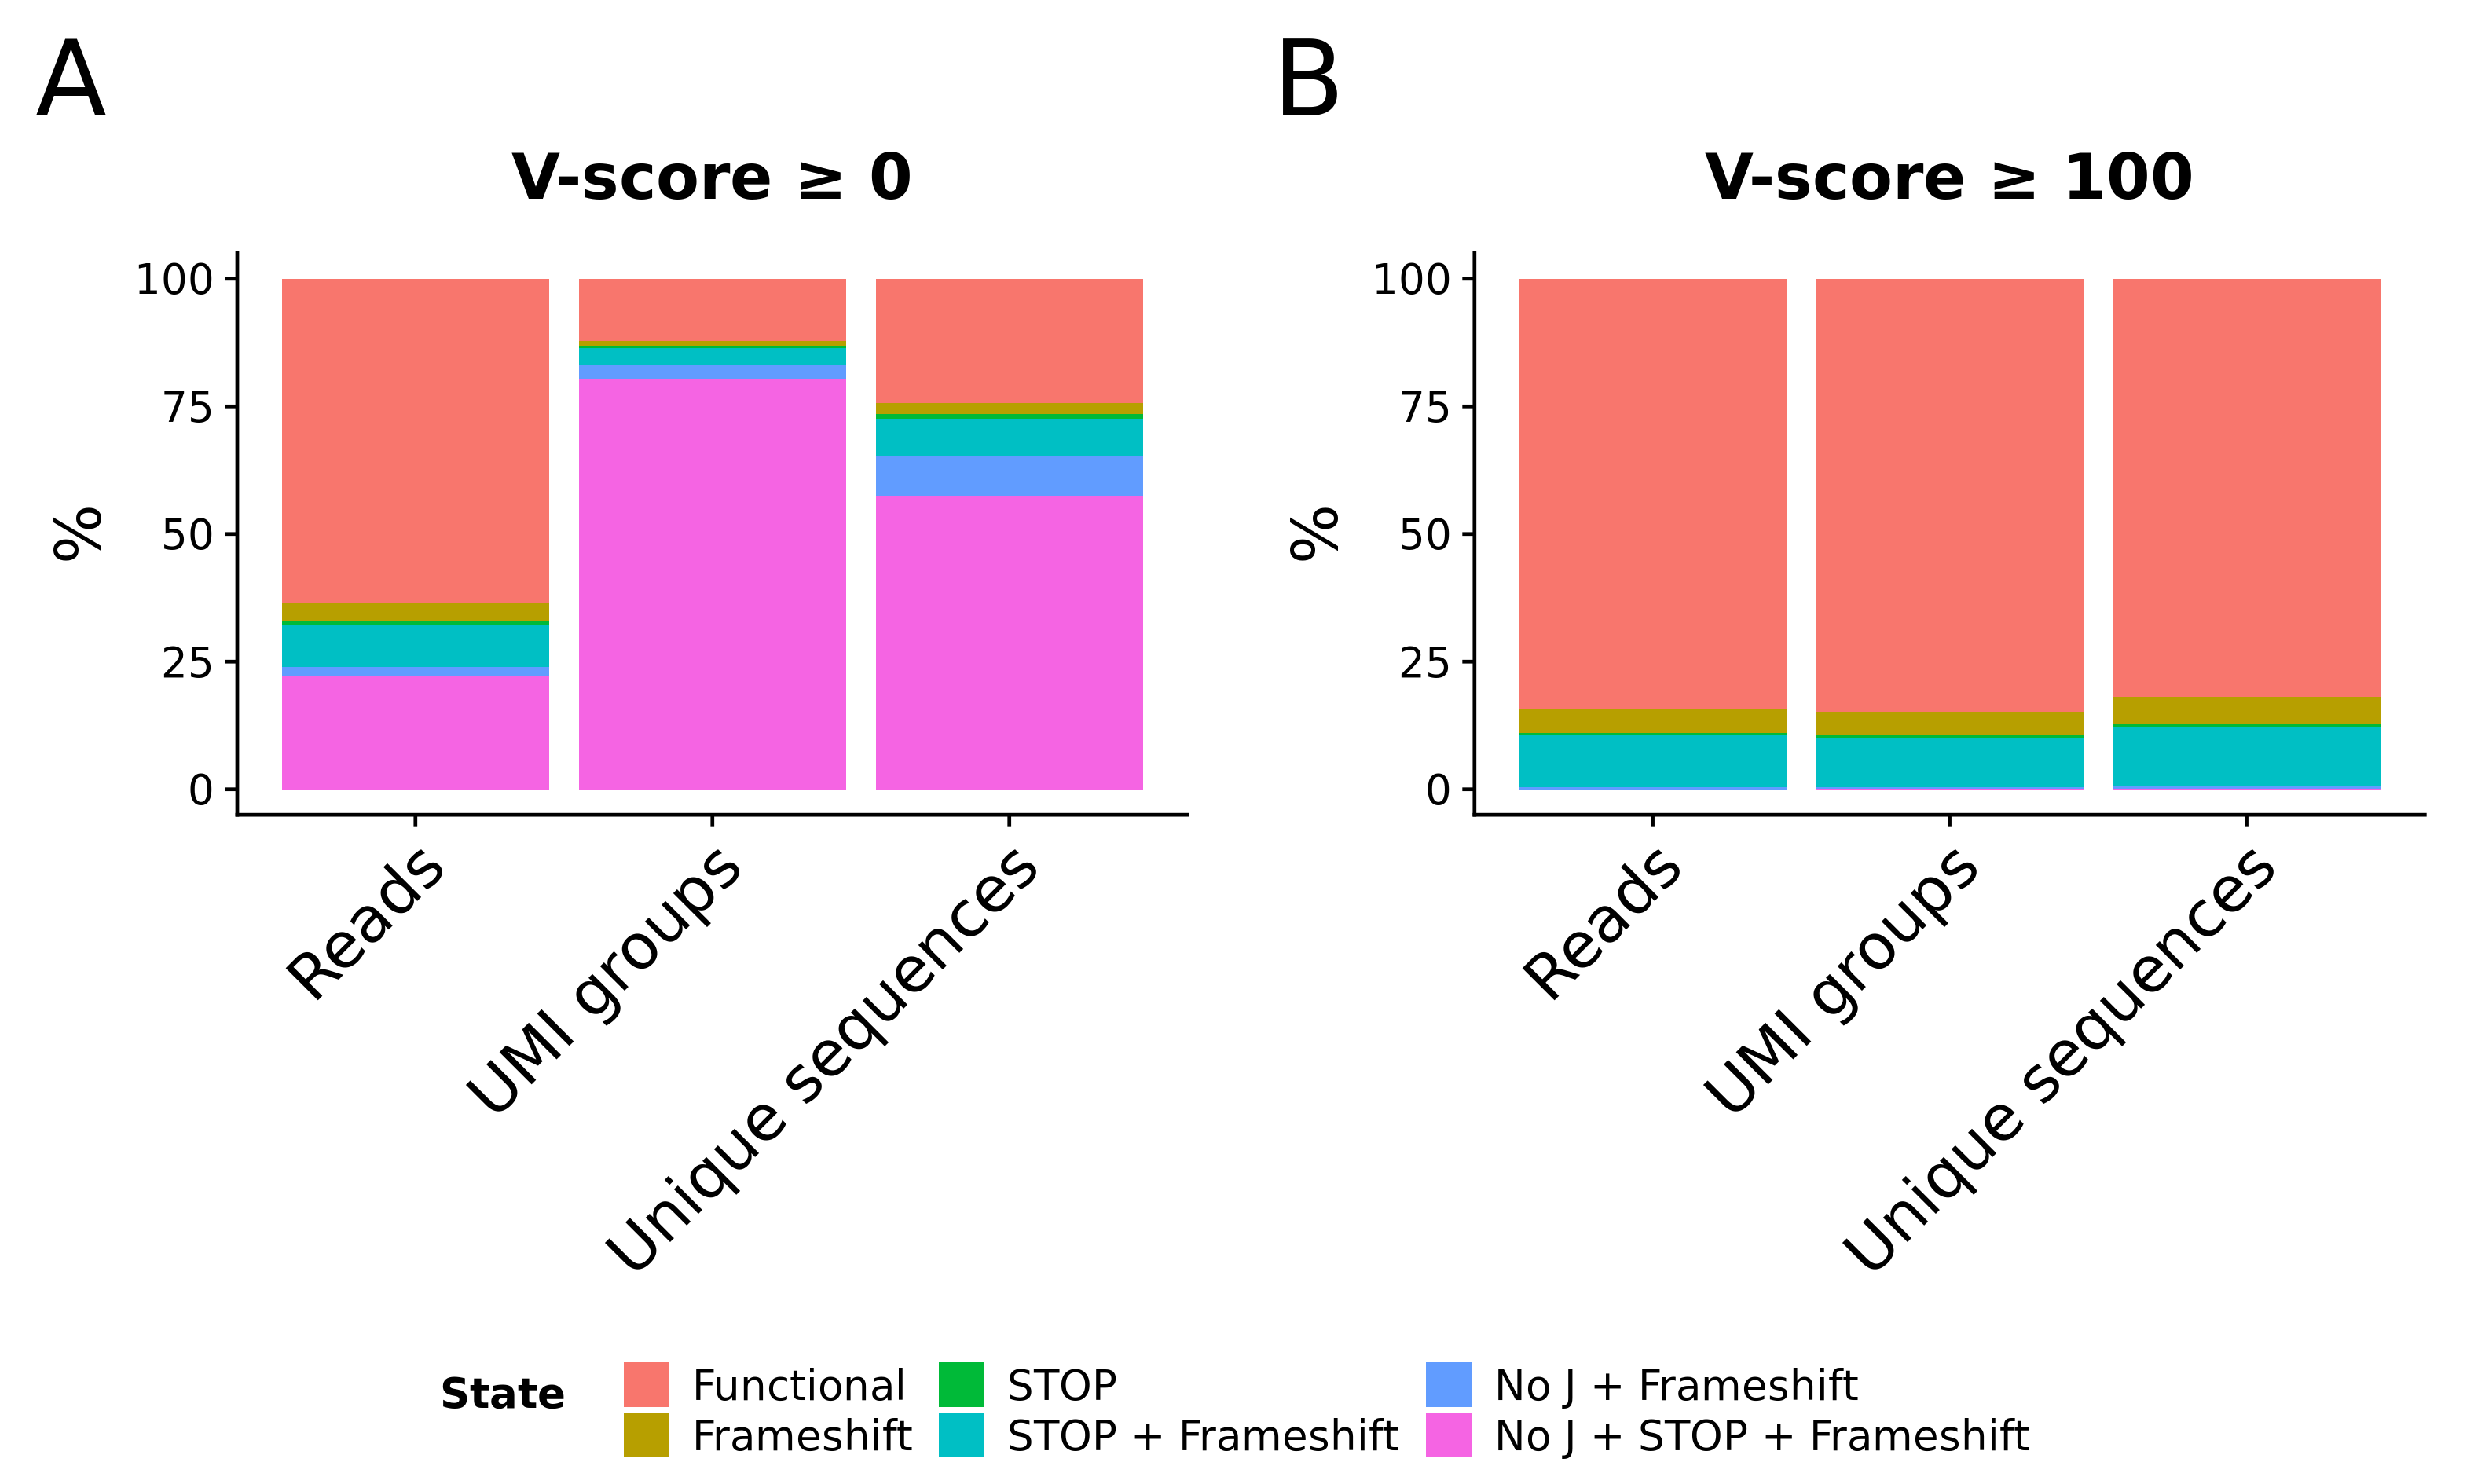
\includegraphics[width = 0.9\textwidth]{_Figures/png/ageing-functional-prop}
\begin{subfigure}{0em}
\phantomsubcaption{}
\label{fig:igseq-ageing-functional-prop-pre}
\end{subfigure}
\begin{subfigure}{0em}
\phantomsubcaption{}
\label{fig:igseq-ageing-functional-prop-post}
\end{subfigure}
\Caption{Functional composition and V-score filtering in the \igseq ageing dataset}{Proportion of input reads, UMI groups and unique sequences in the \igseq ageing dataset belonging to different (non)functional categories, before (A) and after (B) filtering on V-alignment score.}
\label{fig:igseq-ageing-functional-prop}
\end{figure}

\begin{figure}
\centering
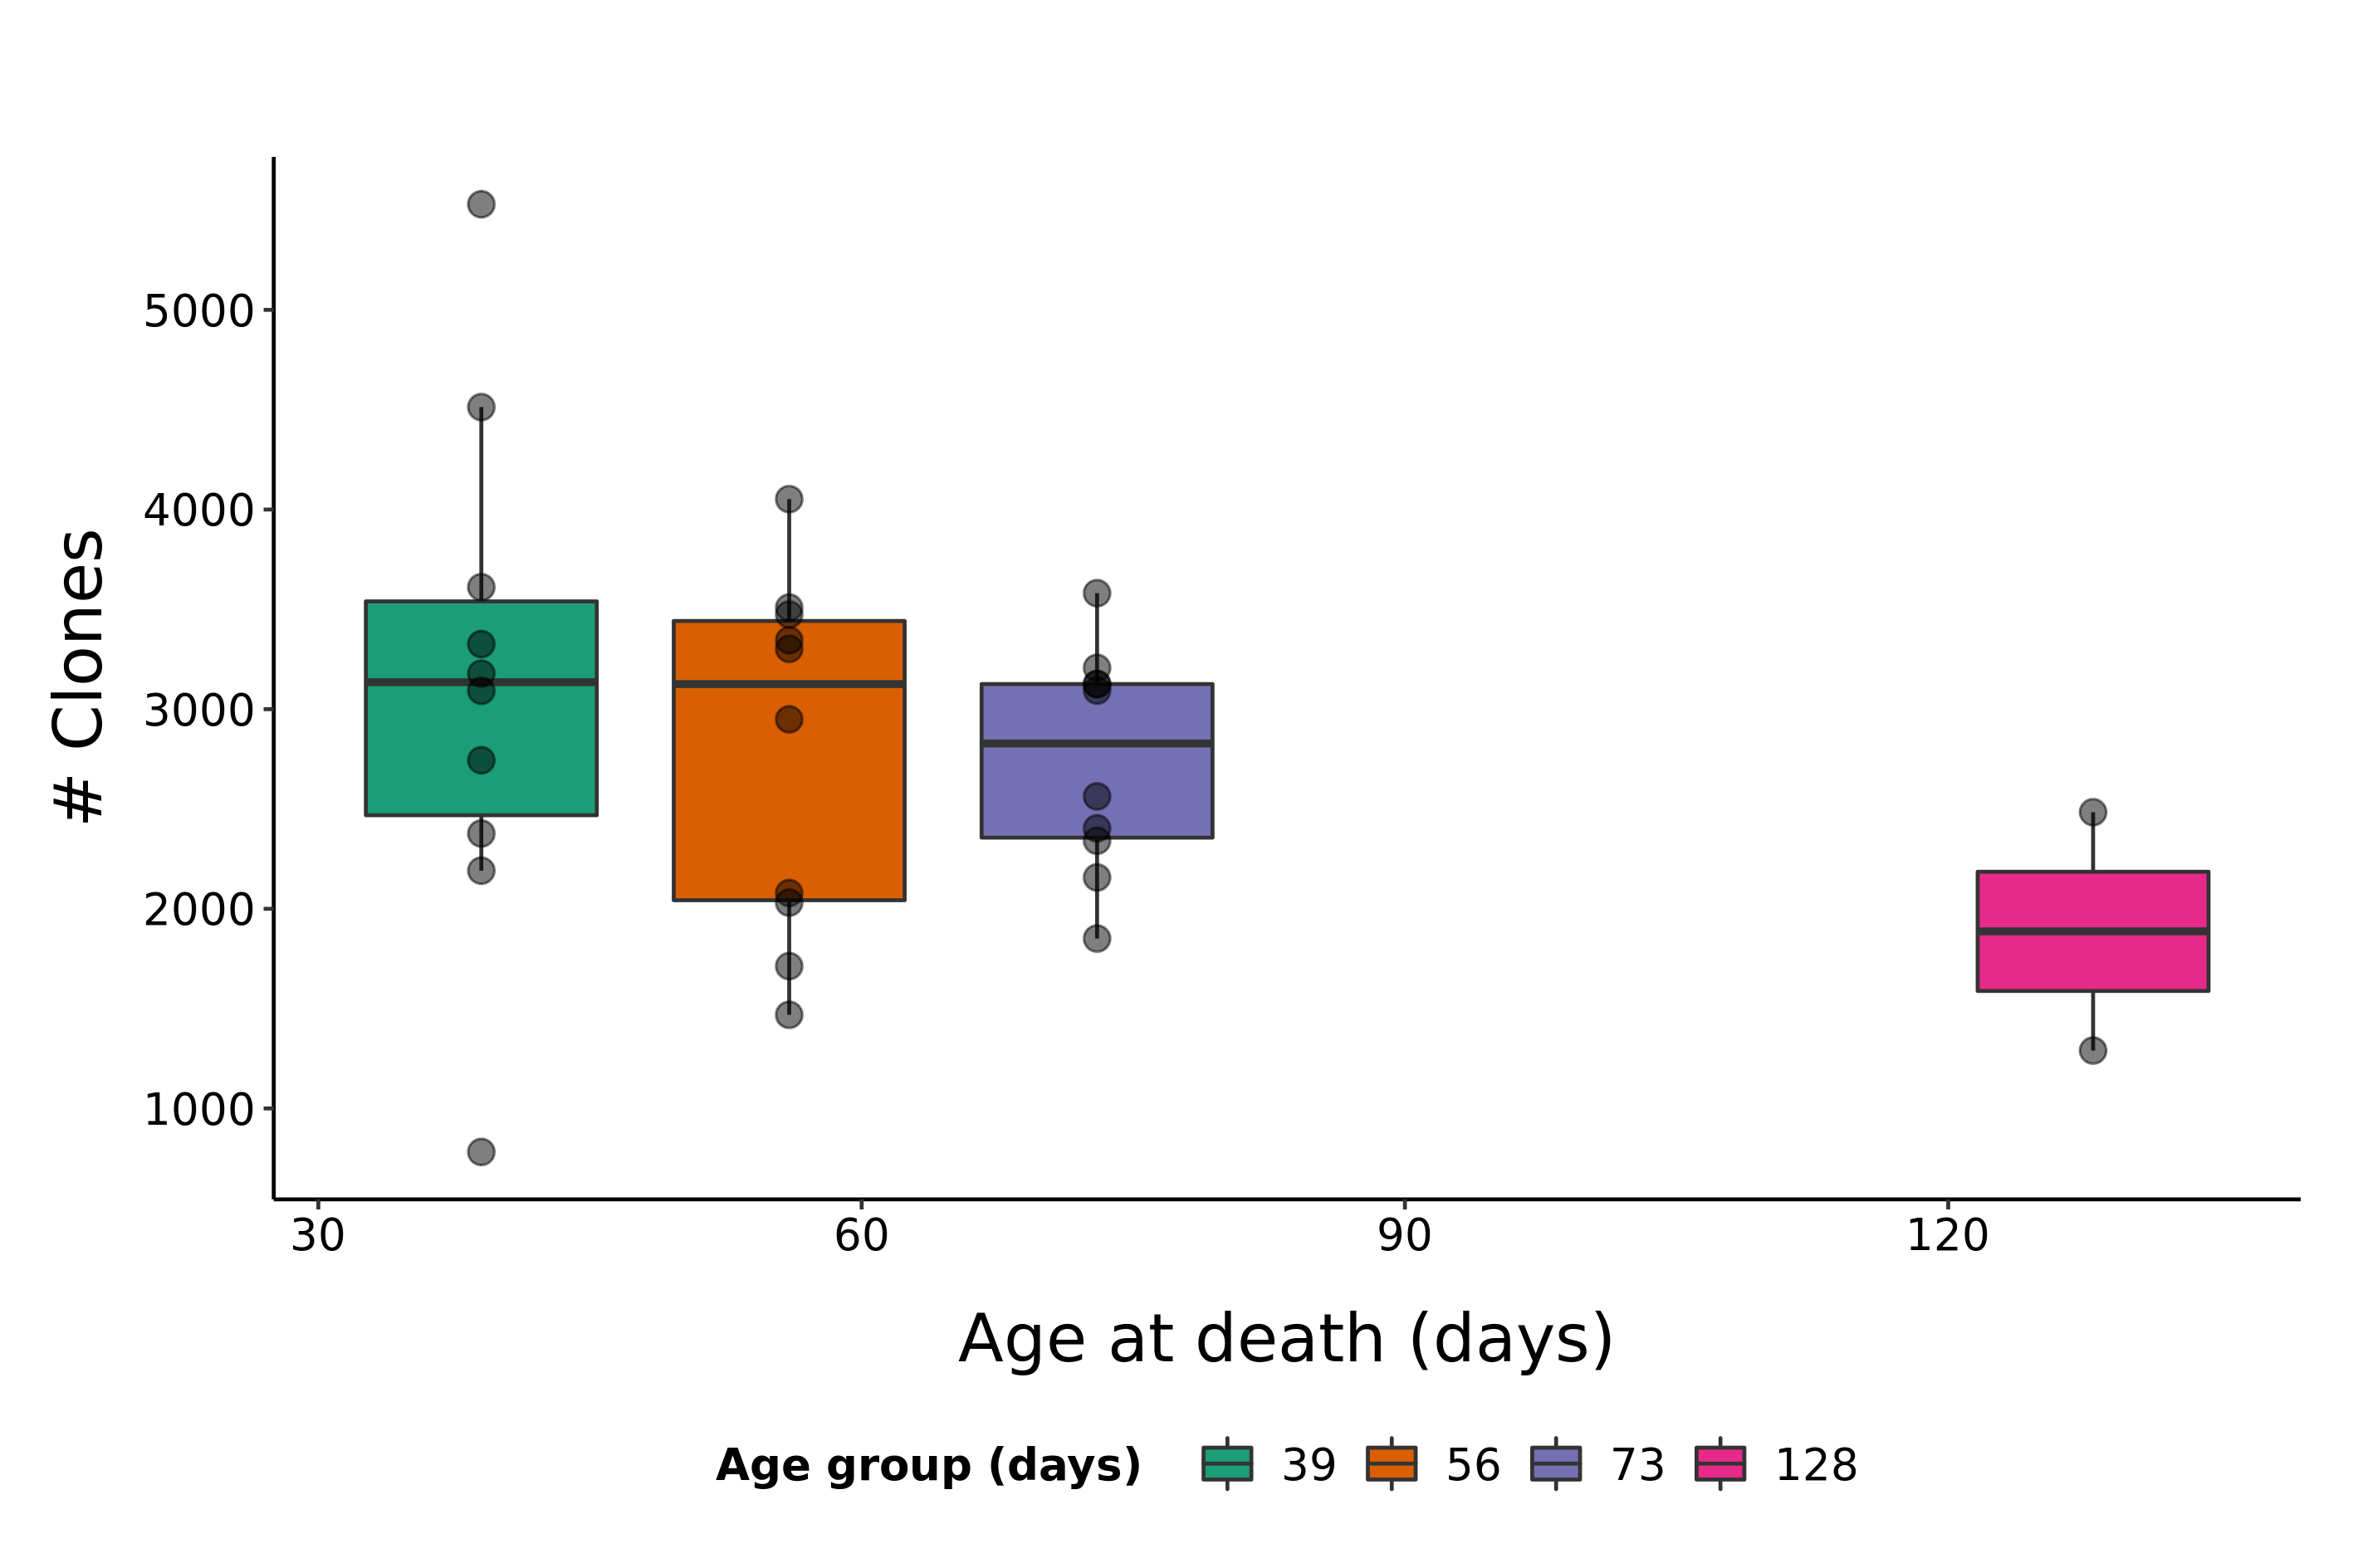
\includegraphics[width = 0.8\textwidth]{/home/will/Documents/thesis/_Figures/png/ageing-nclones.png}
\Caption{Number of clones in the \igseq ageing dataset}{Boxplots of clonal counts for each individual in the \igseq ageing dataset, grouped by age at death. The apparent decline in clonal count with age is not significant (Kruskal-Wallis analysis of variance, $p=\embed{_Figures/txt/ageing-nclones-kruskal-p.txt}$).}
\label{fig:igseq-ageing-nclones}
\end{figure}

\begin{figure}
\centering
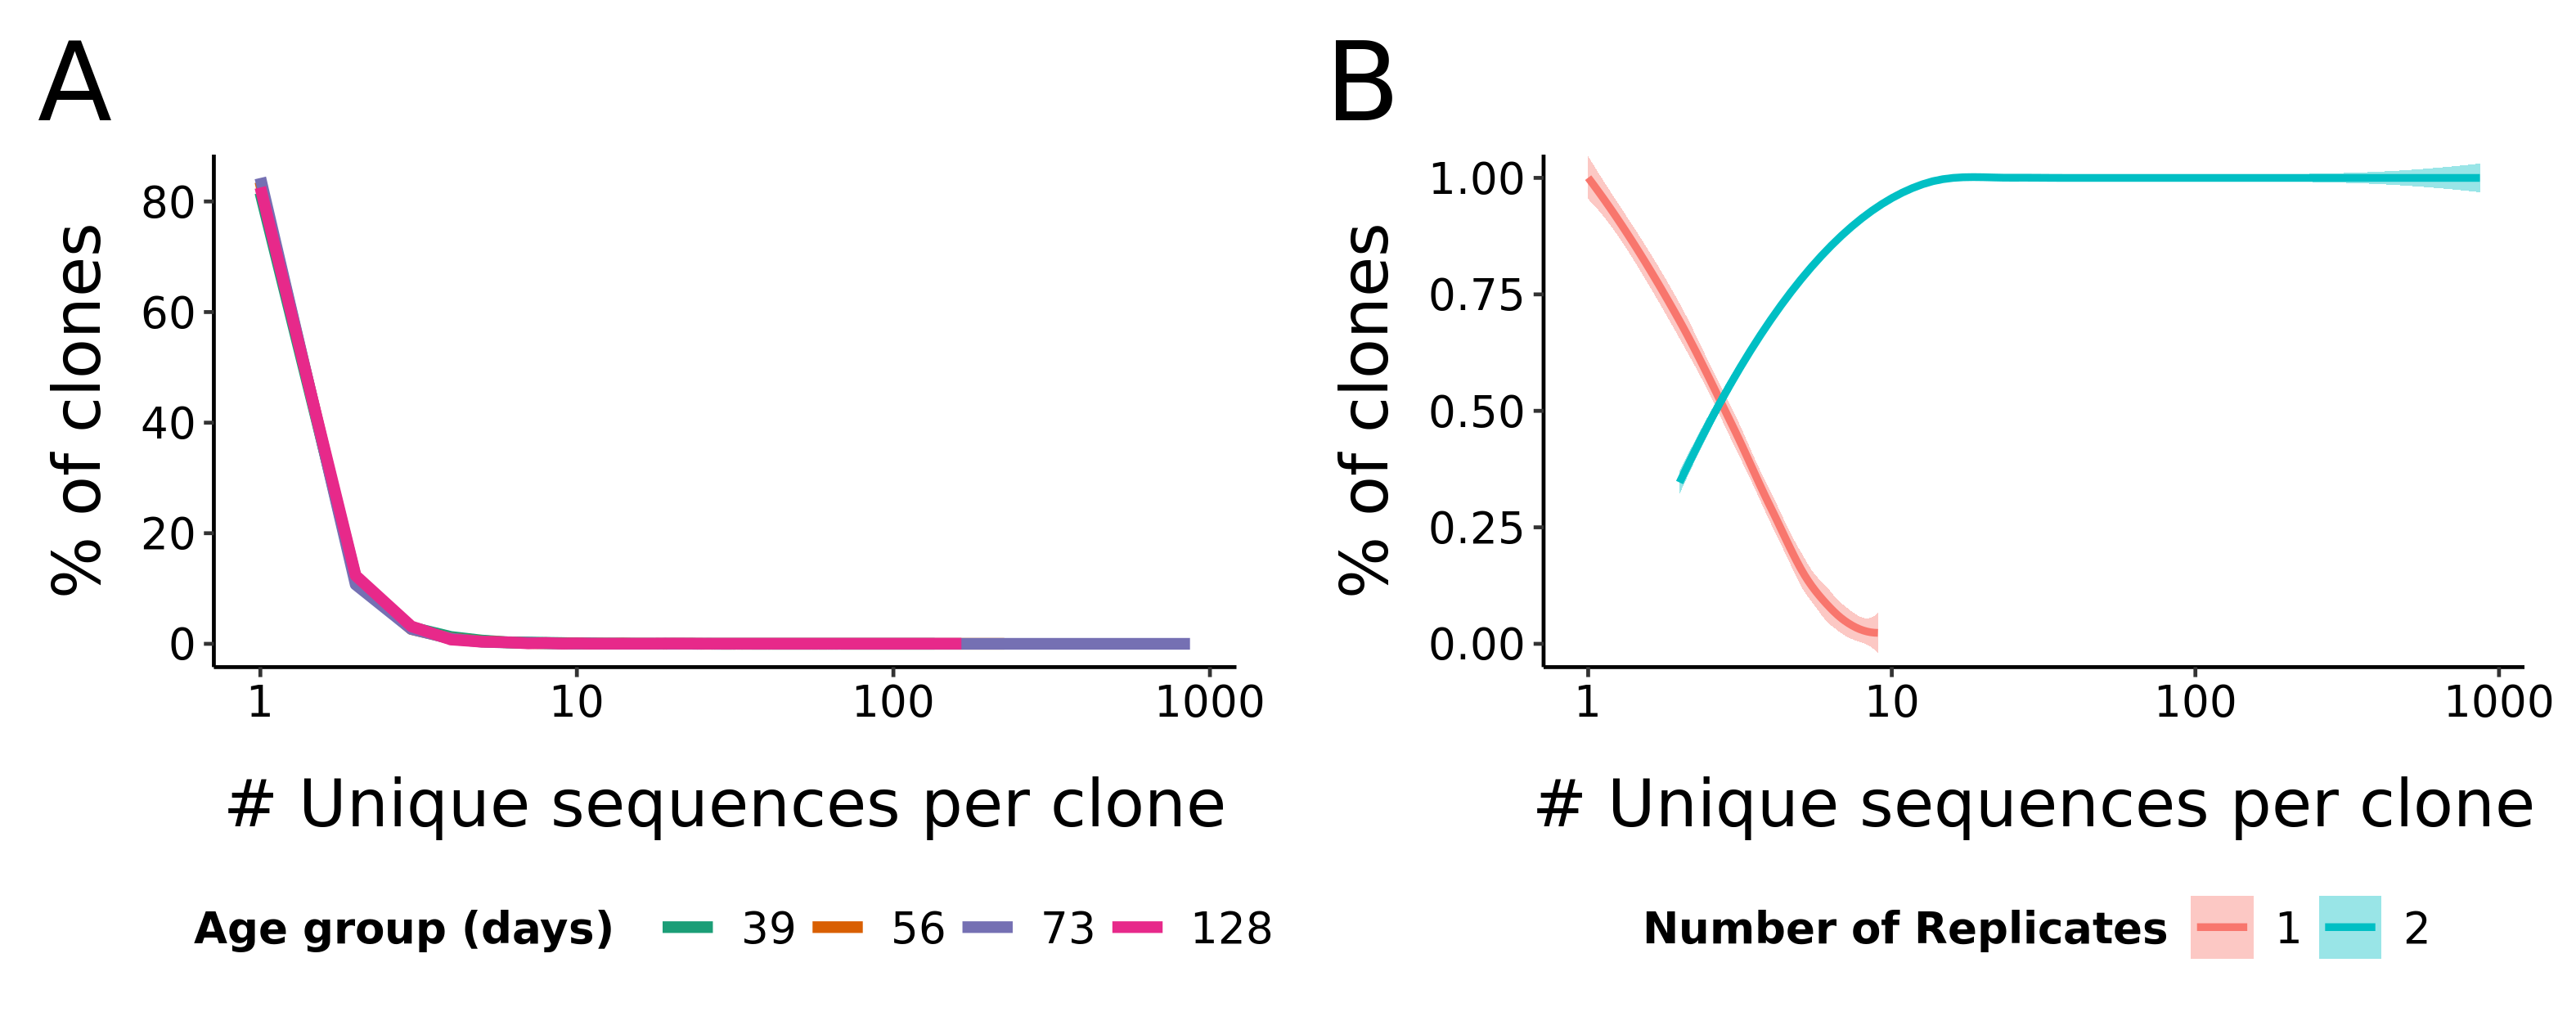
\includegraphics[width = 0.9\textwidth]{_Figures/png/ageing-clone-sizes}
\begin{subfigure}{0em}
\phantomsubcaption{}
\label{fig:igseq-ageing-clone-sizes-sizes}
\end{subfigure}
\begin{subfigure}{0em}
\phantomsubcaption{}
\label{fig:igseq-ageing-clone-sizes-reps}
\end{subfigure}
\Caption{Clone size and cross-replicate reproducibility in the \igseq ageing dataset}{(A) Proportion of clones of different sizes for each individual in the \igseq ageing dataset, measured in unique sequences per clone. (B) LOESS-smoothed curves \parencite{cleveland1991loess} showing proportion of clones of each size found across one or both replicates of the appropriate individual.}
\label{fig:igseq-ageing-clone-sizes}
\end{figure}

\begin{figure}
\centering
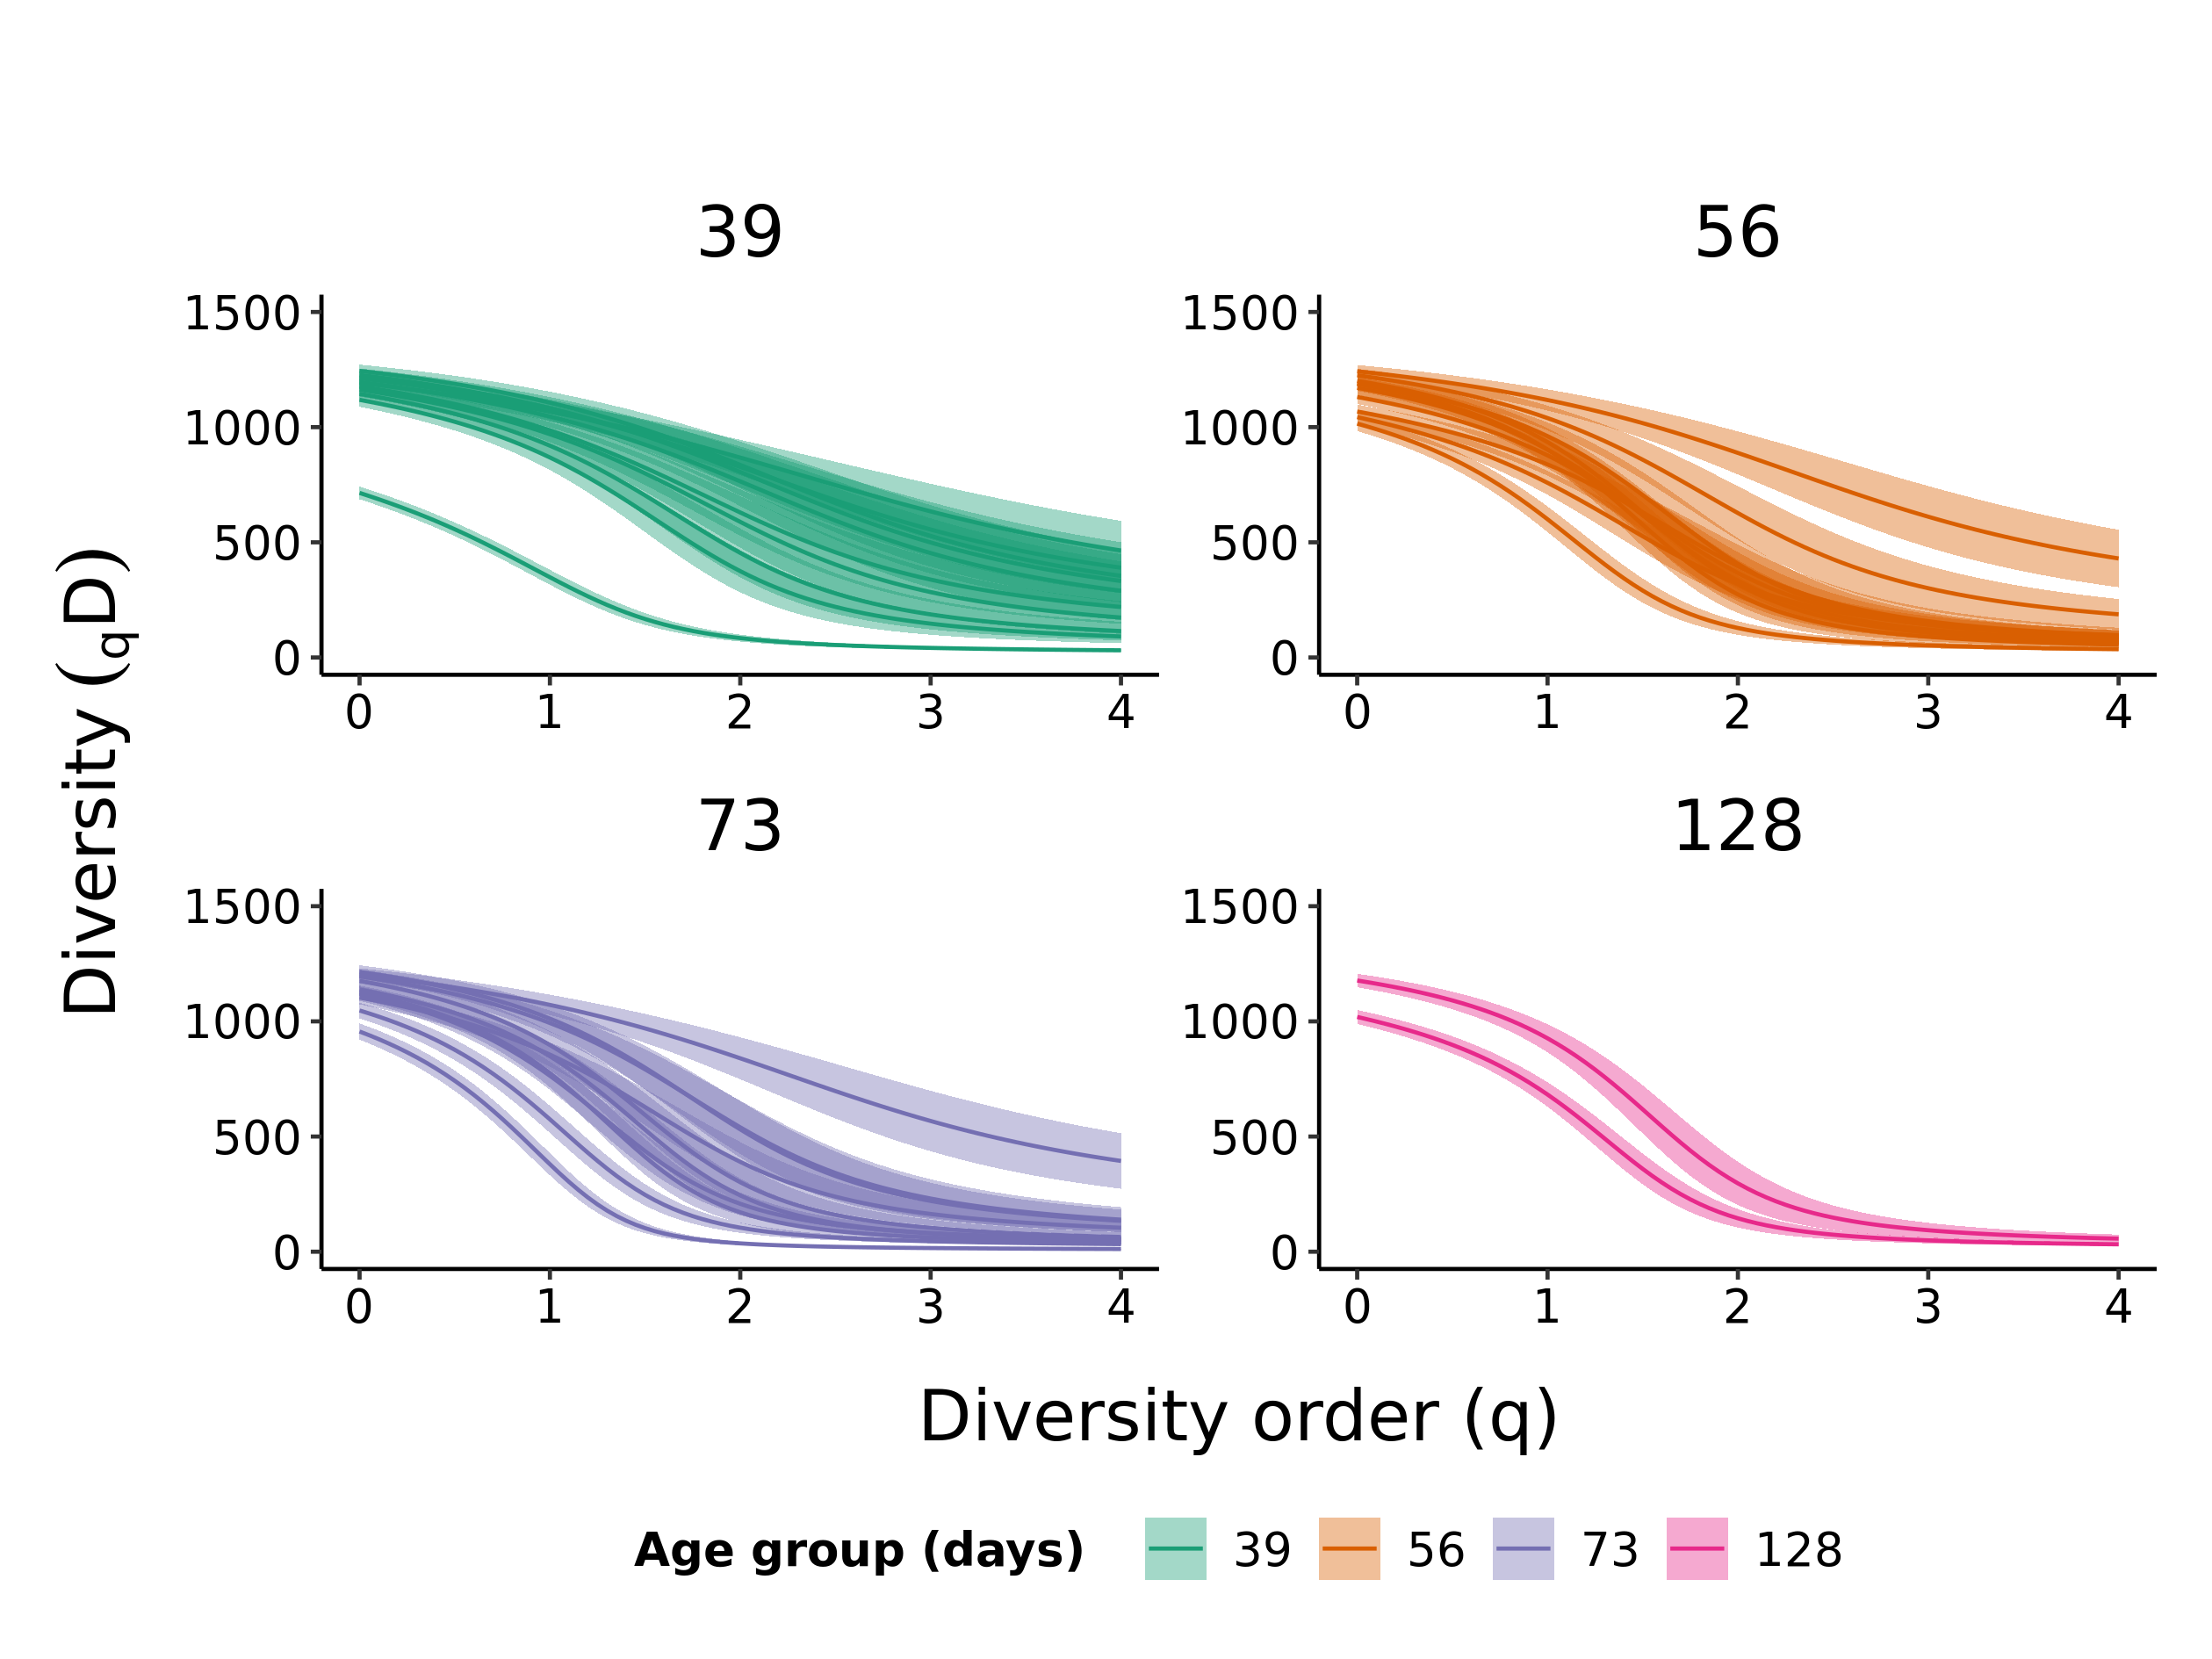
\includegraphics[width = 0.8\textwidth]{_Figures/png/ageing-clone-diversity-solo-spectra}
\Caption{Per-individual clonal-diversity spectra in the \igseq ageing dataset}{Hill diversity spectra of clone sizes (as measured by number of unique sequences per clone) for each individual in the \igseq ageing dataset, grouped by age at death.}
\label{fig:igseq-ageing-clone-diversity-solo-spectra}
\end{figure}

\begin{figure}
\centering
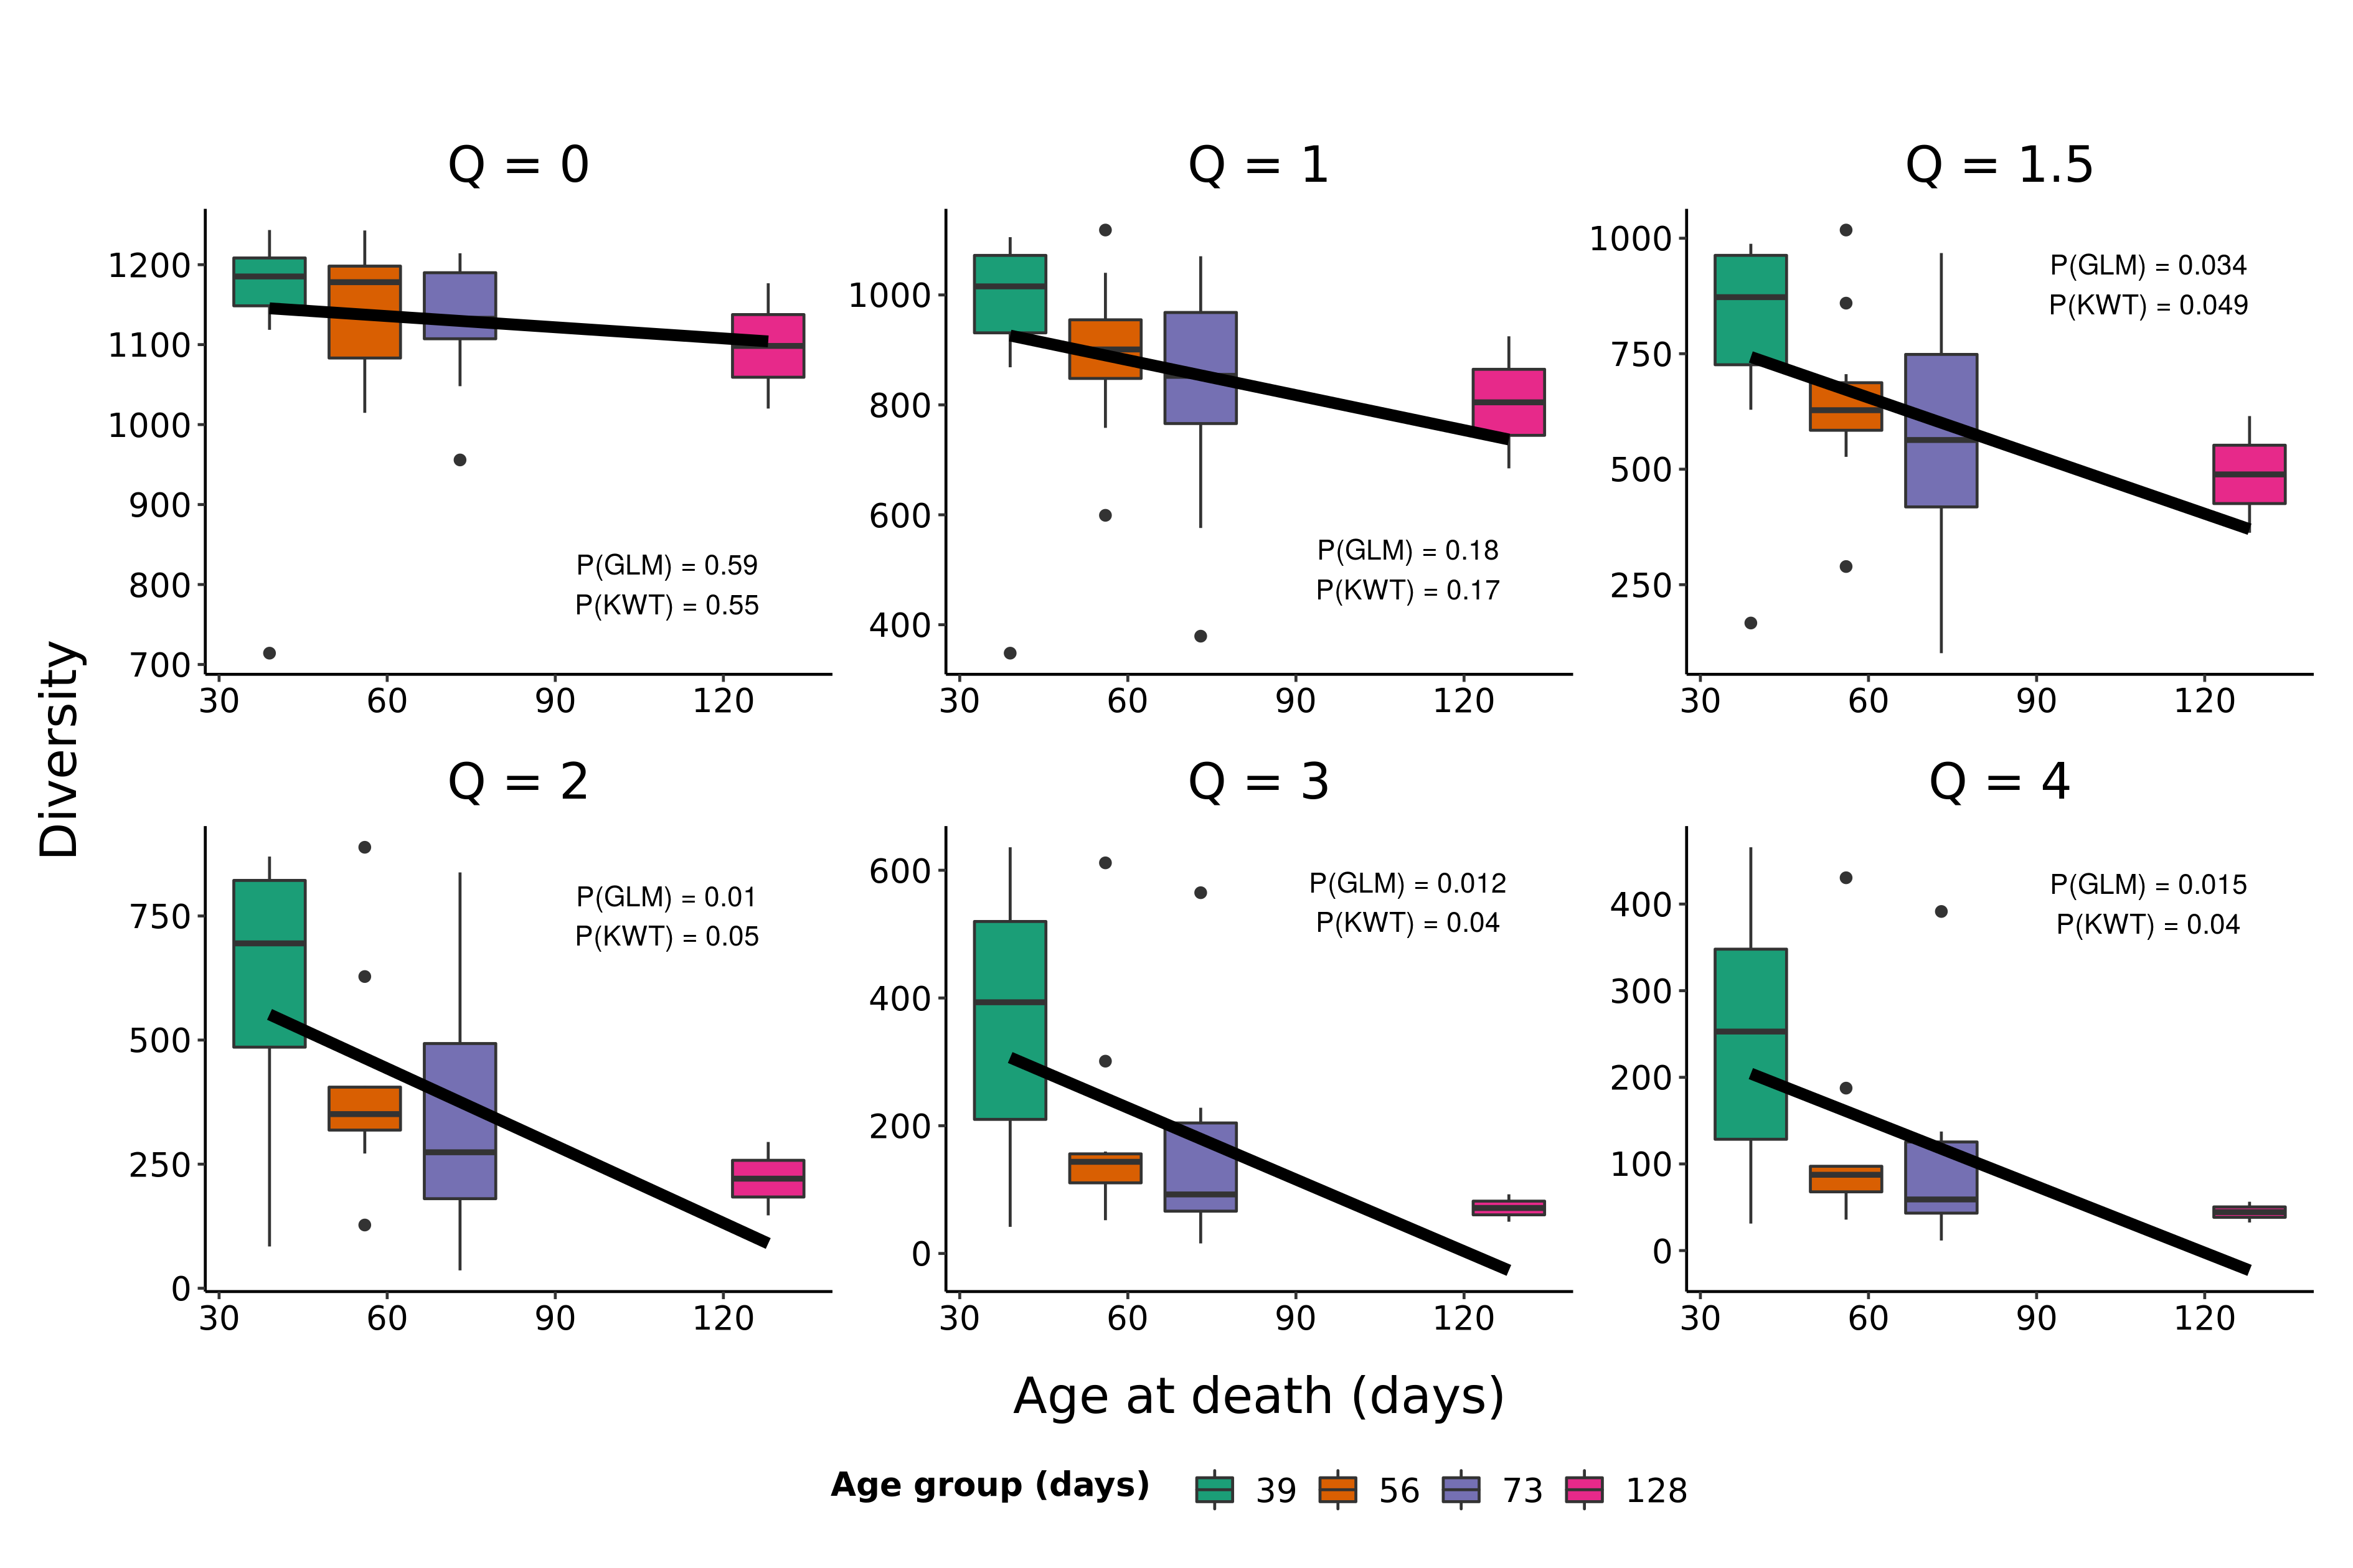
\includegraphics[width = 0.8\textwidth]{_Figures/png/ageing-clone-diversity-solo-fit-linear}
\Caption{Comparing clonal alpha-diversities between age groups in the \igseq ageing dataset (linear fit)}{Boxplots of Hill diversity values for the antibody repertoires of individuals of each age group in the \igseq ageing dataset at a sample of diversity orders, overlaid with the predictions of the best-fit linear model at each order.  Annotated $p$-values indicate the statistical significance of the estimated age effect on diversity under the linear model ($P(GLM)$) and a Kruskal-Wallis test ($P(KWT)$) for each diversity order.}
\label{fig:igseq-ageing-clone-diversity-solo-fit-linear}
\end{figure}

\begin{figure}
\centering
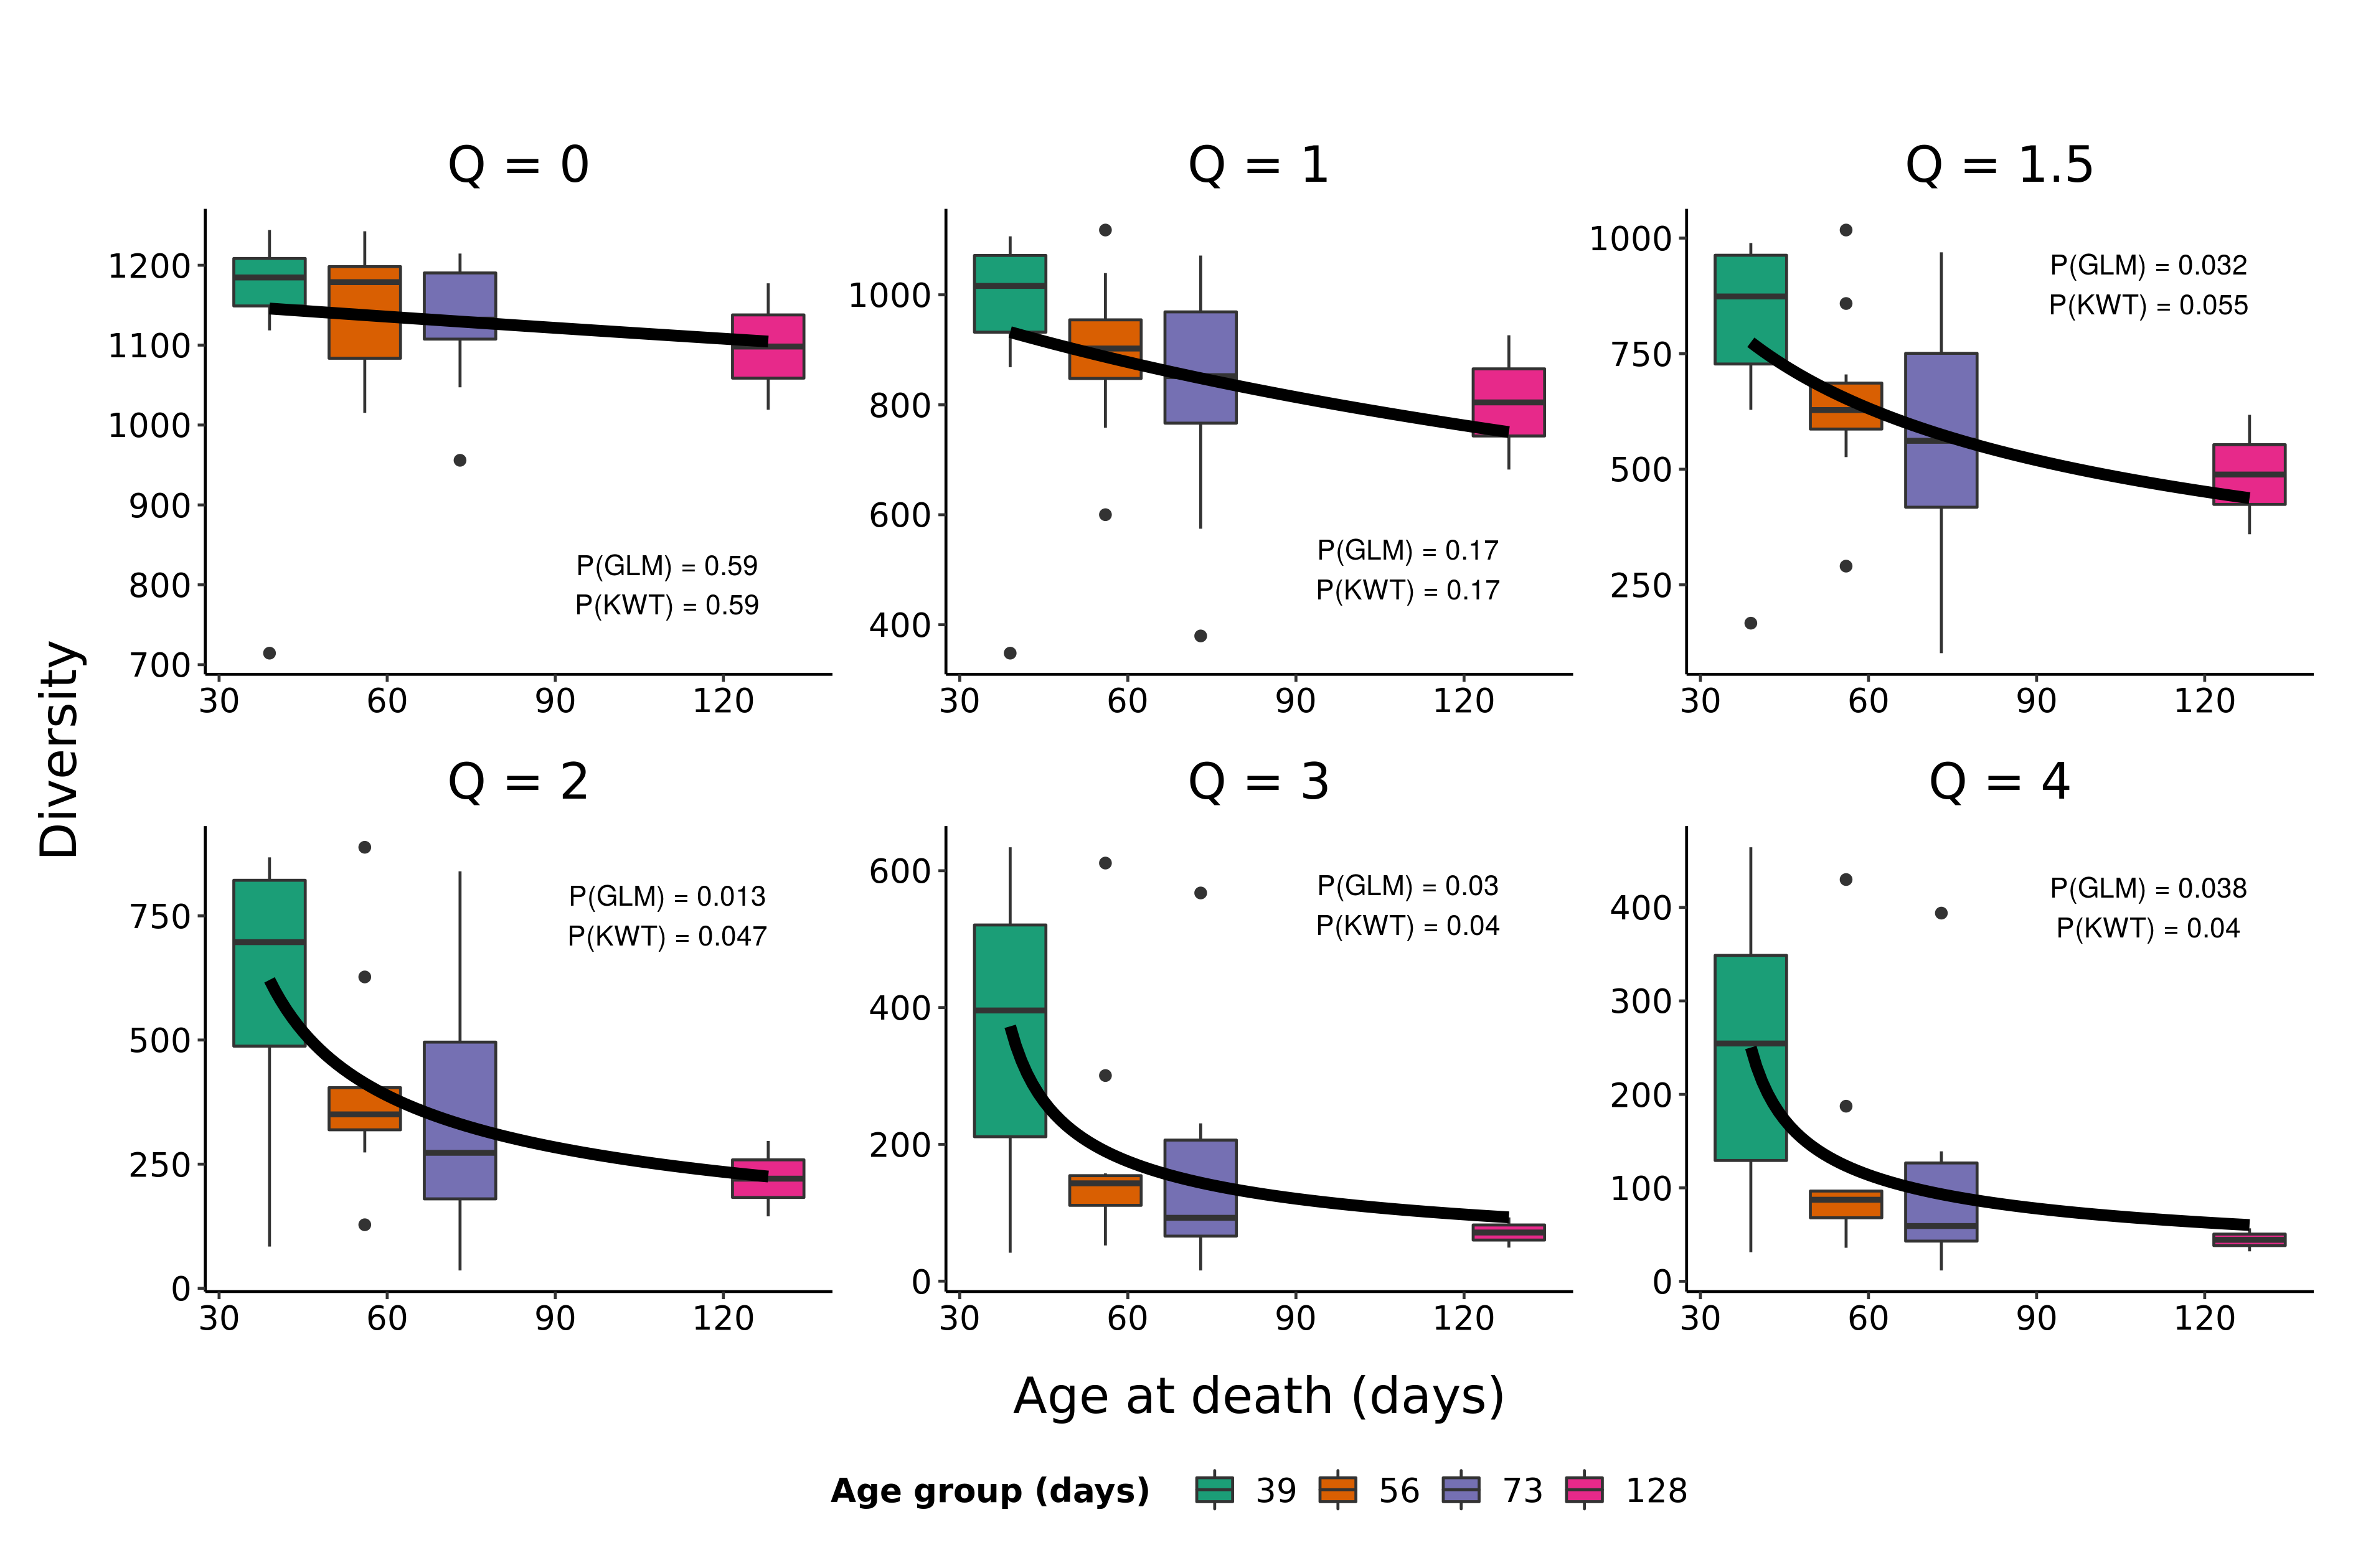
\includegraphics[width = 0.8\textwidth]{_Figures/png/ageing-clone-diversity-solo-fit-igauss}
\Caption{Comparing clonal alpha-diversities between age groups in the \igseq ageing dataset (inverse-Gaussian fit)}{Boxplots of Hill diversity values for the antibody repertoires of individuals of each age group in the \igseq ageing dataset at a sample of diversity orders, overlaid with the predictions of the best-fit inverse-Gaussian-distributed generalised linear model at each order.  Annotated $p$-values indicate the statistical significance of the estimated age effect on diversity under the GLM ($P(GLM)$) and a Kruskal-Wallis test ($P(KWT)$) for each diversity order.}
\label{fig:igseq-ageing-clone-diversity-solo-fit-igauss}
\end{figure}

\begin{figure}
\centering
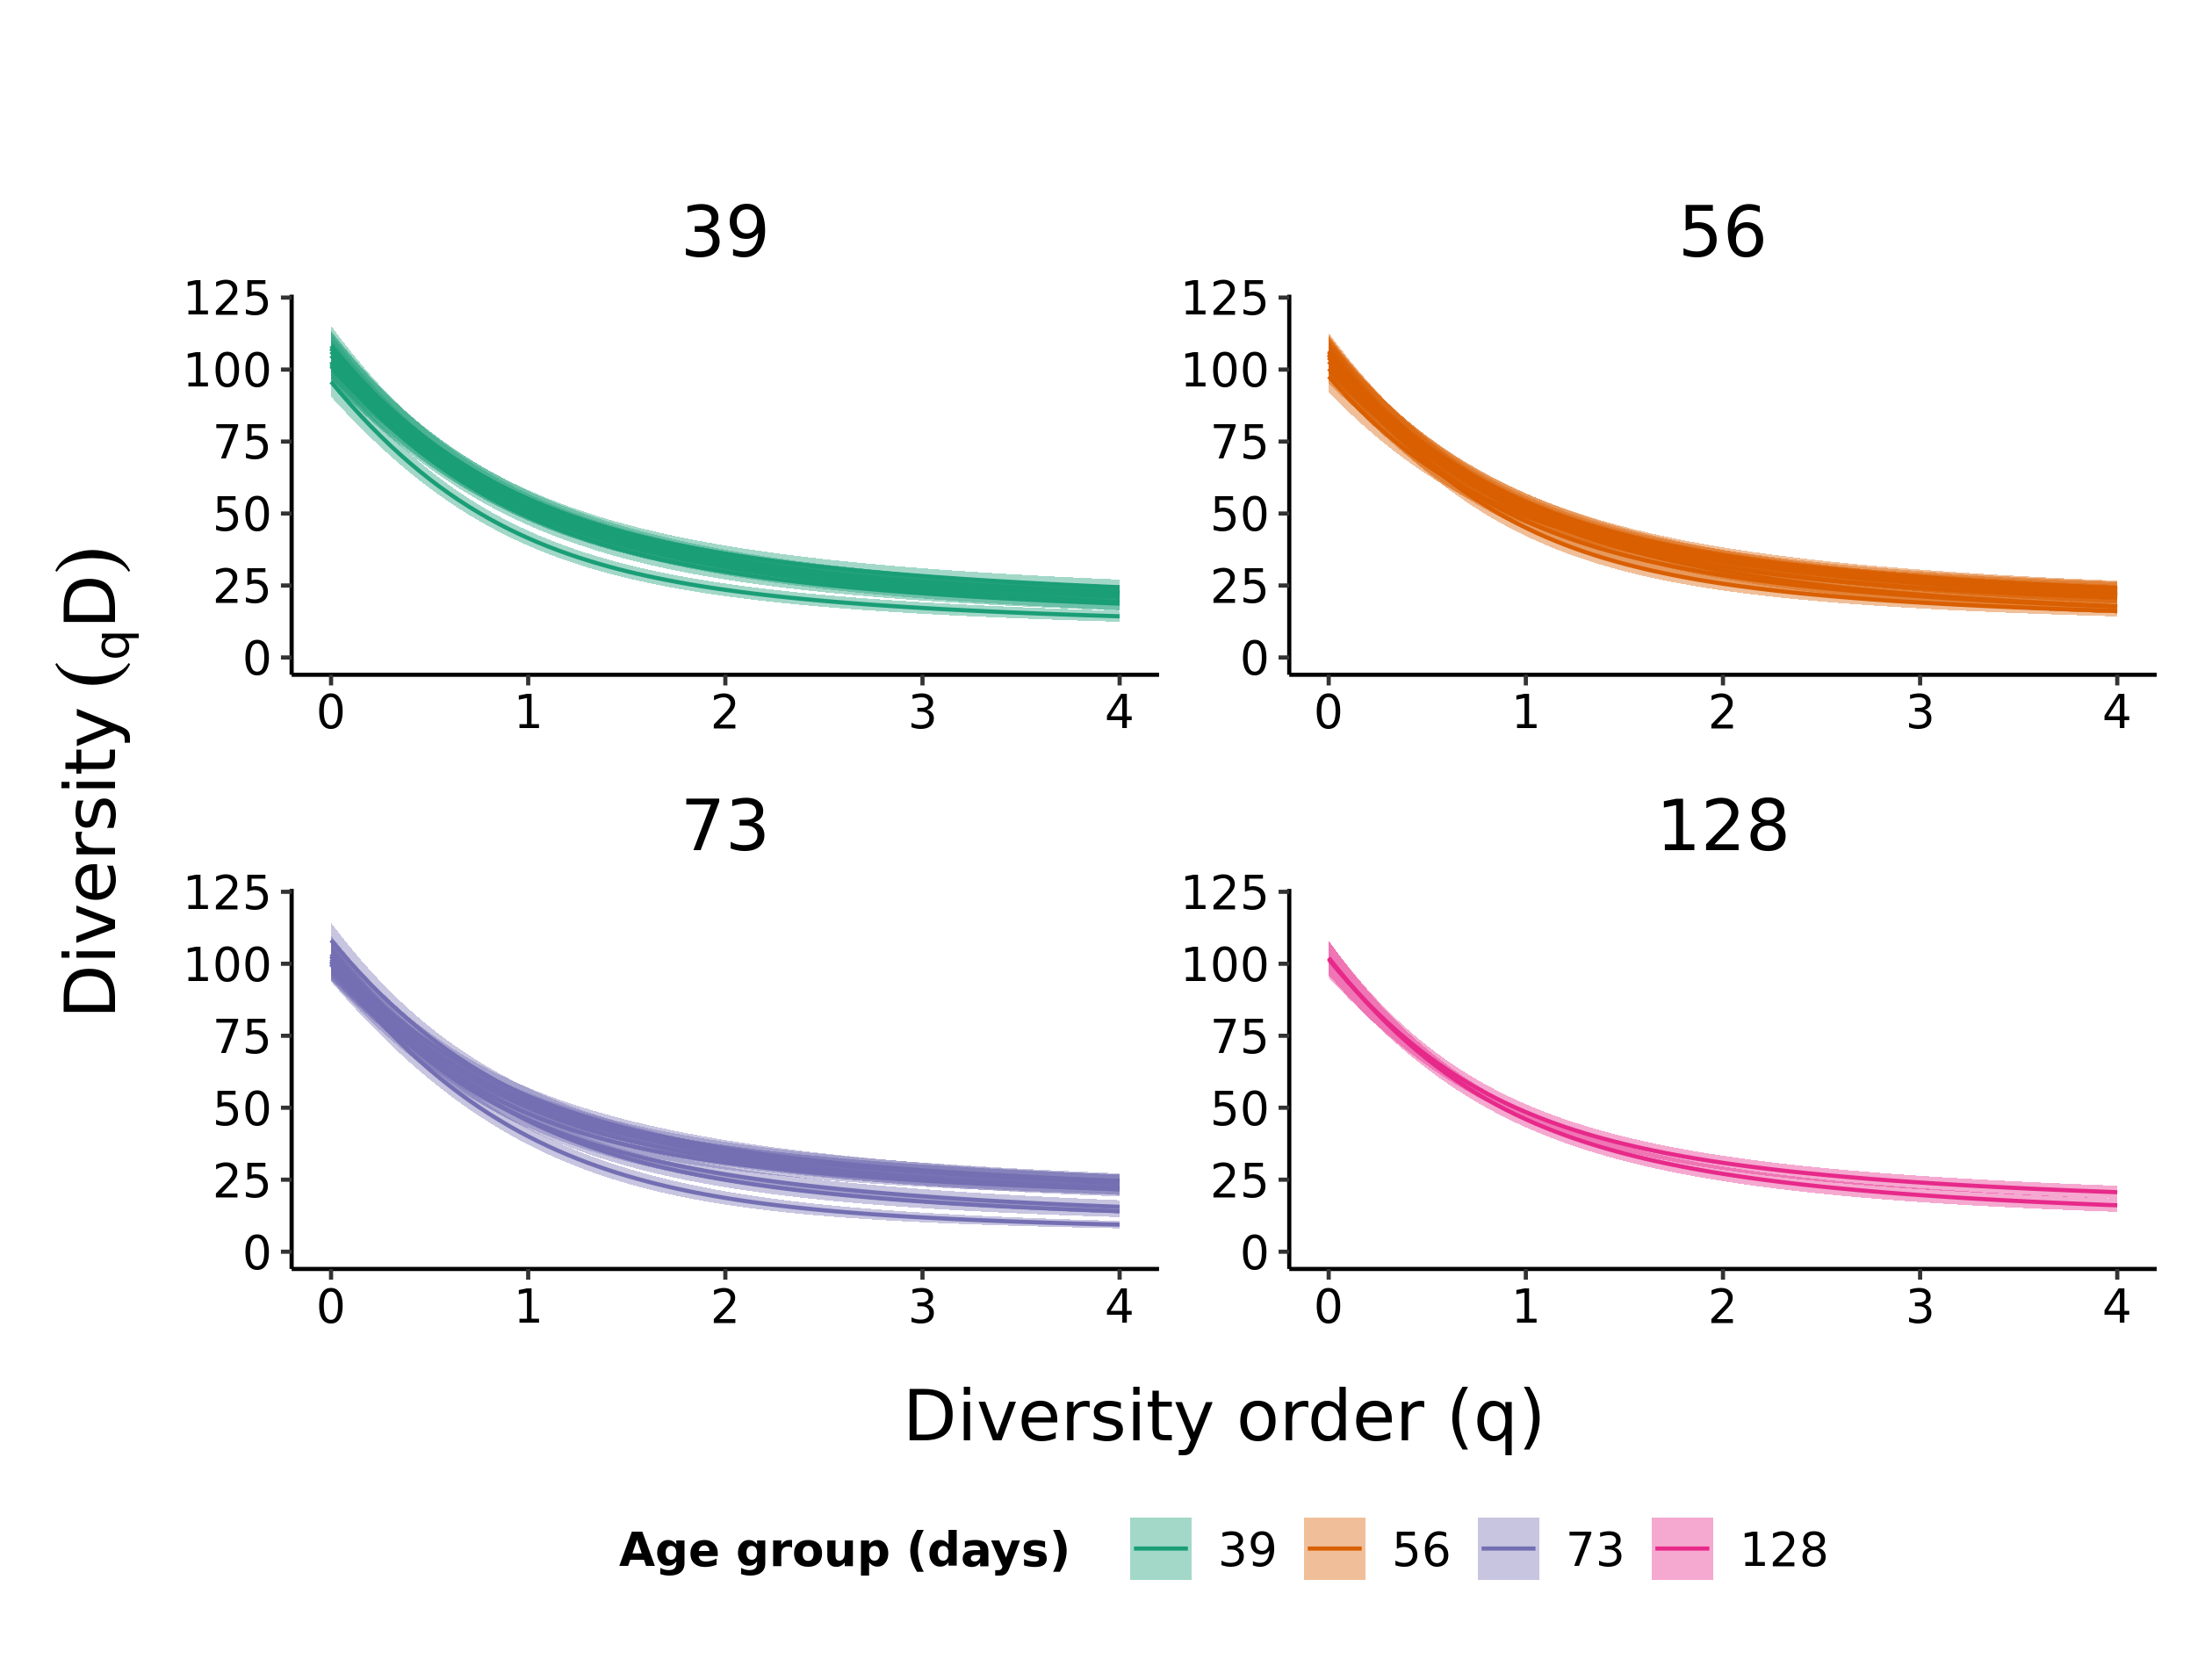
\includegraphics[width = 0.8\textwidth]{_Figures/png/ageing-VJ-diversity-solo-spectra}
\Caption{Per-individual VJ-diversity spectra for the \igseq ageing dataset}{Hill diversity spectra of VJ usage (as measured by number of unique sequences per V/J combination) for each individual in the \igseq ageing dataset, grouped by age at death.}
\label{fig:igseq-ageing-vj-diversity-solo-spectra}
\end{figure}

\begin{figure}
\centering
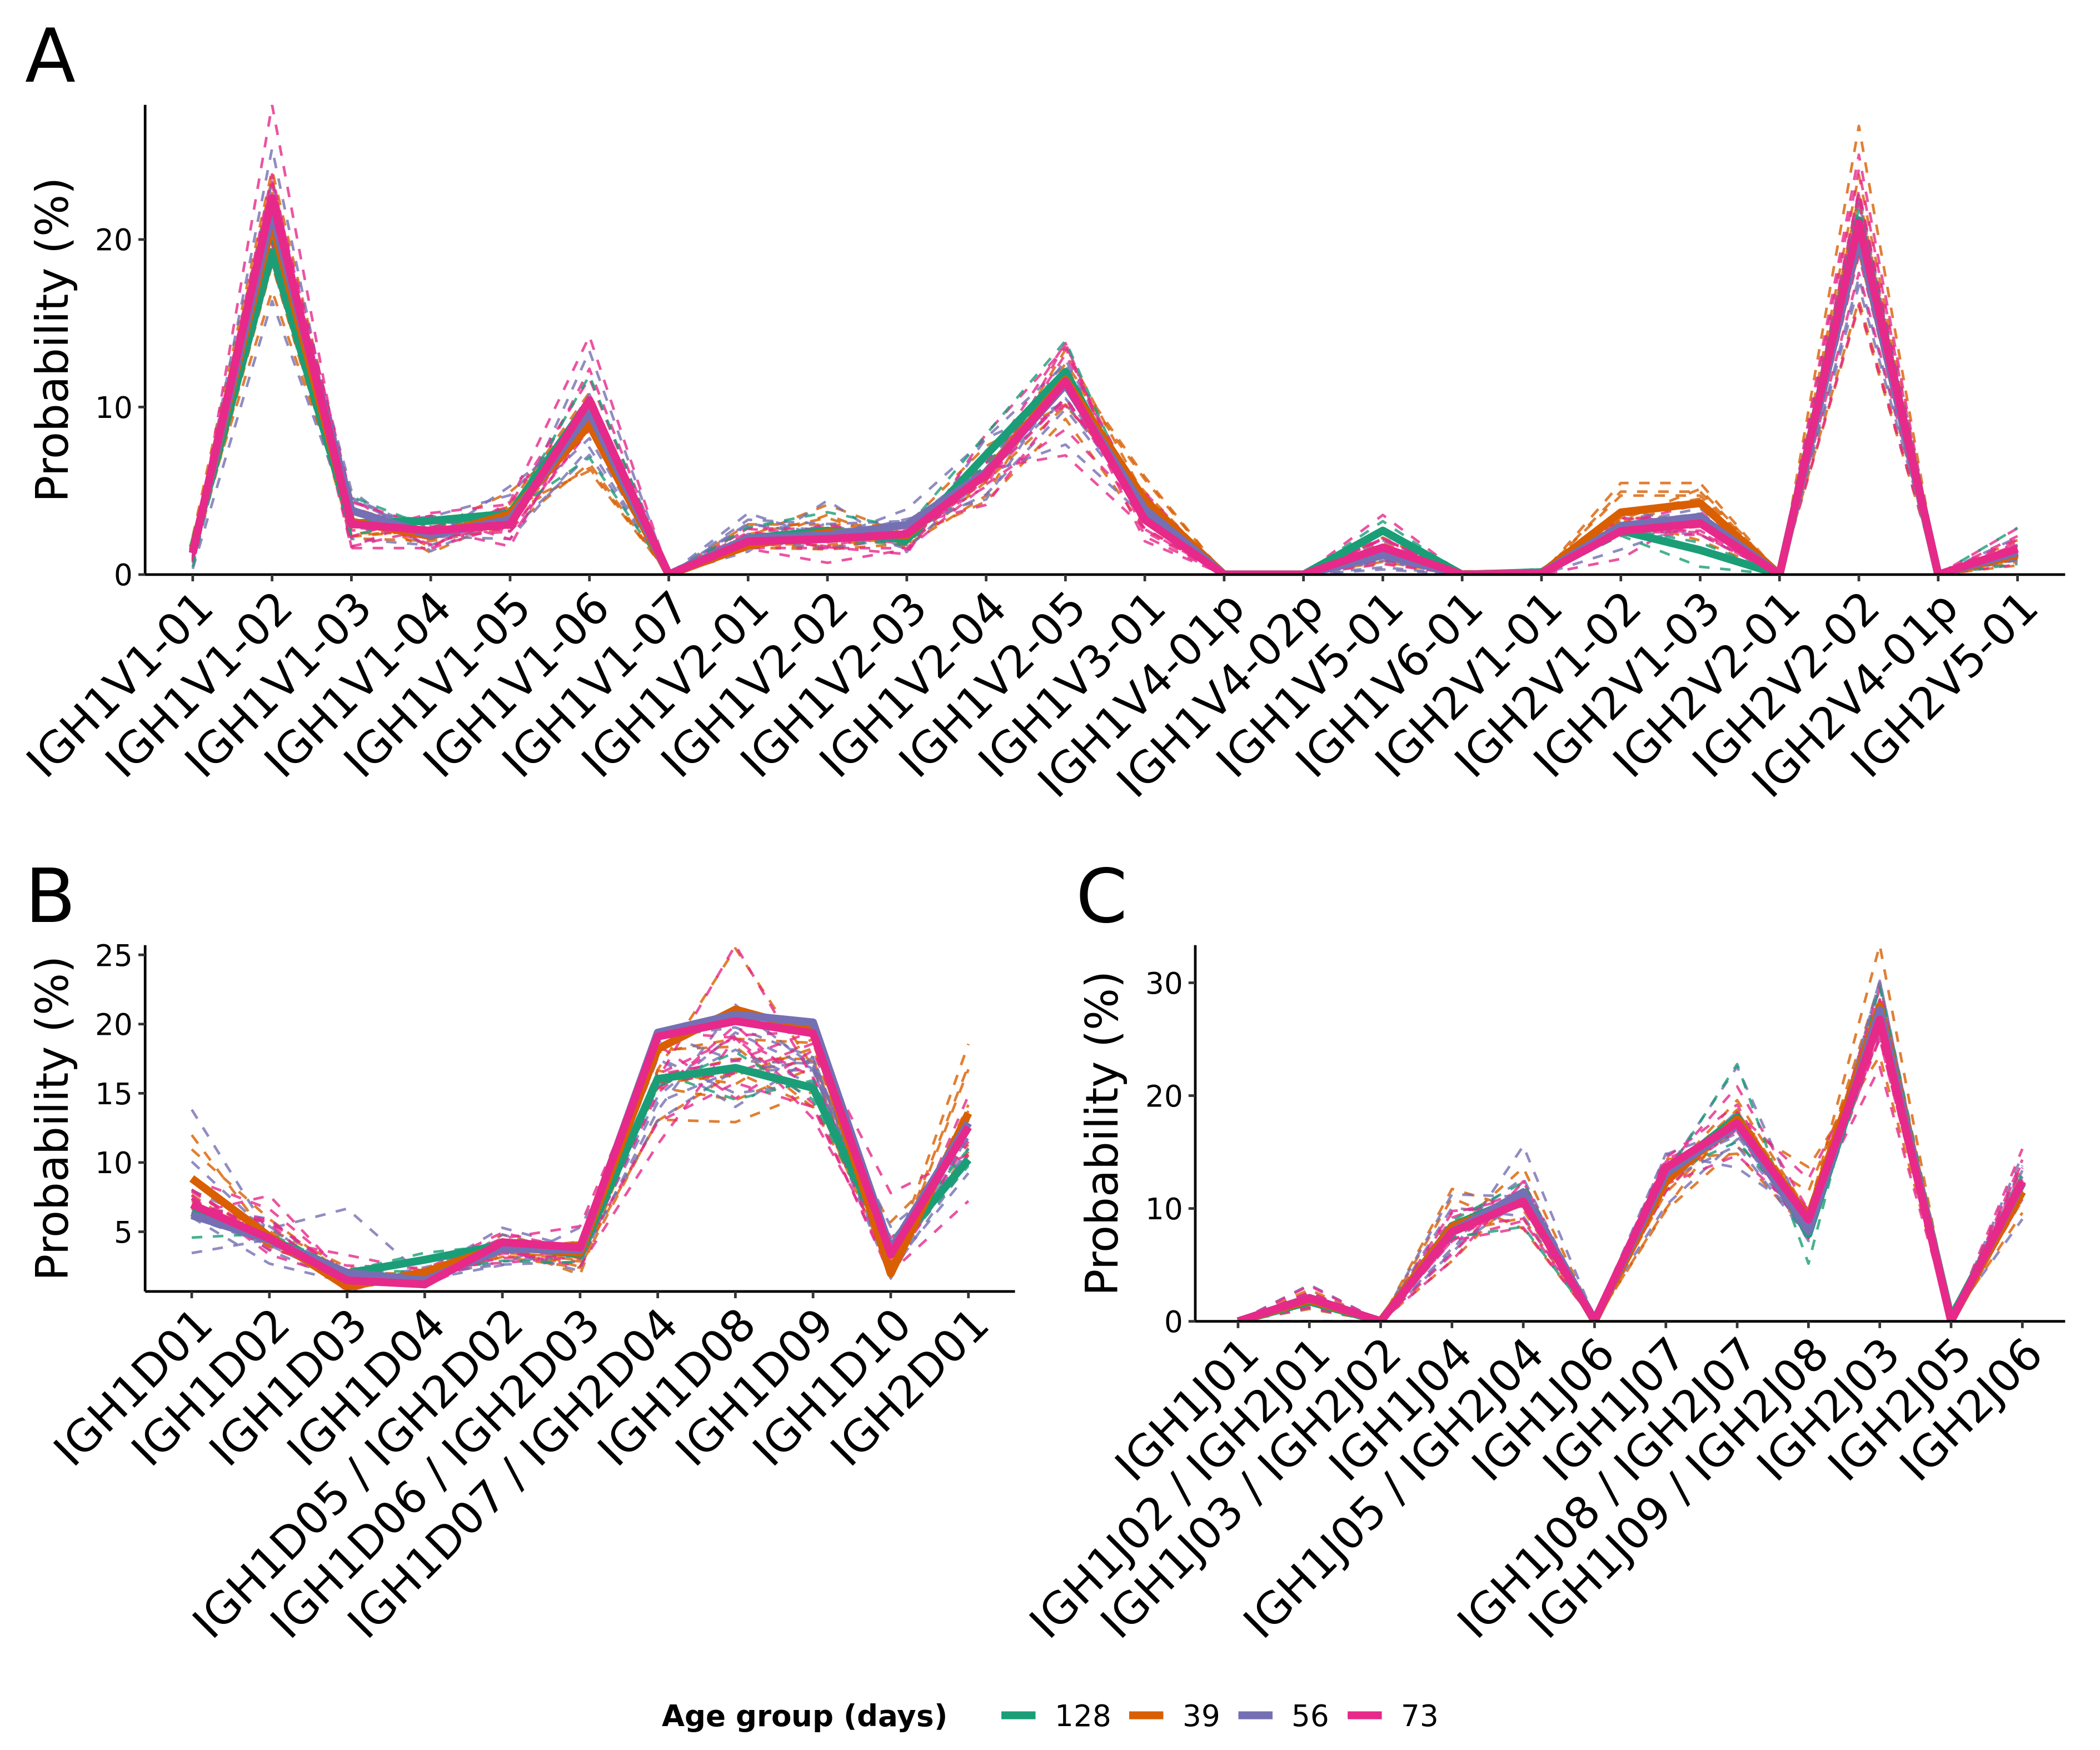
\includegraphics[width = 0.8\textwidth]{_Figures/png/ageing-igor-segments}
\Caption{Generative segment-choice distributions in the \igseq ageing dataset}{Probability distributions of segment choice for (A) \vh-, (B) \dh- and (C) \jh-segments during VDJ recombination in adult male turquoise killifish of different ages, inferred from the \igseq ageing dataset using \program{IGoR}. Thin dashed lines represent the distributions inferred for individual killifish, while the thick solid lines represent those inferred from pooled data from all individuals in each age group. \dh and \jh segments with identical sequences (which cannot be distinguished in the repertoire data even in principle) are collapsed together.}
\label{fig:igseq-ageing-igor-segments}
\end{figure}

\begin{figure}
\centering
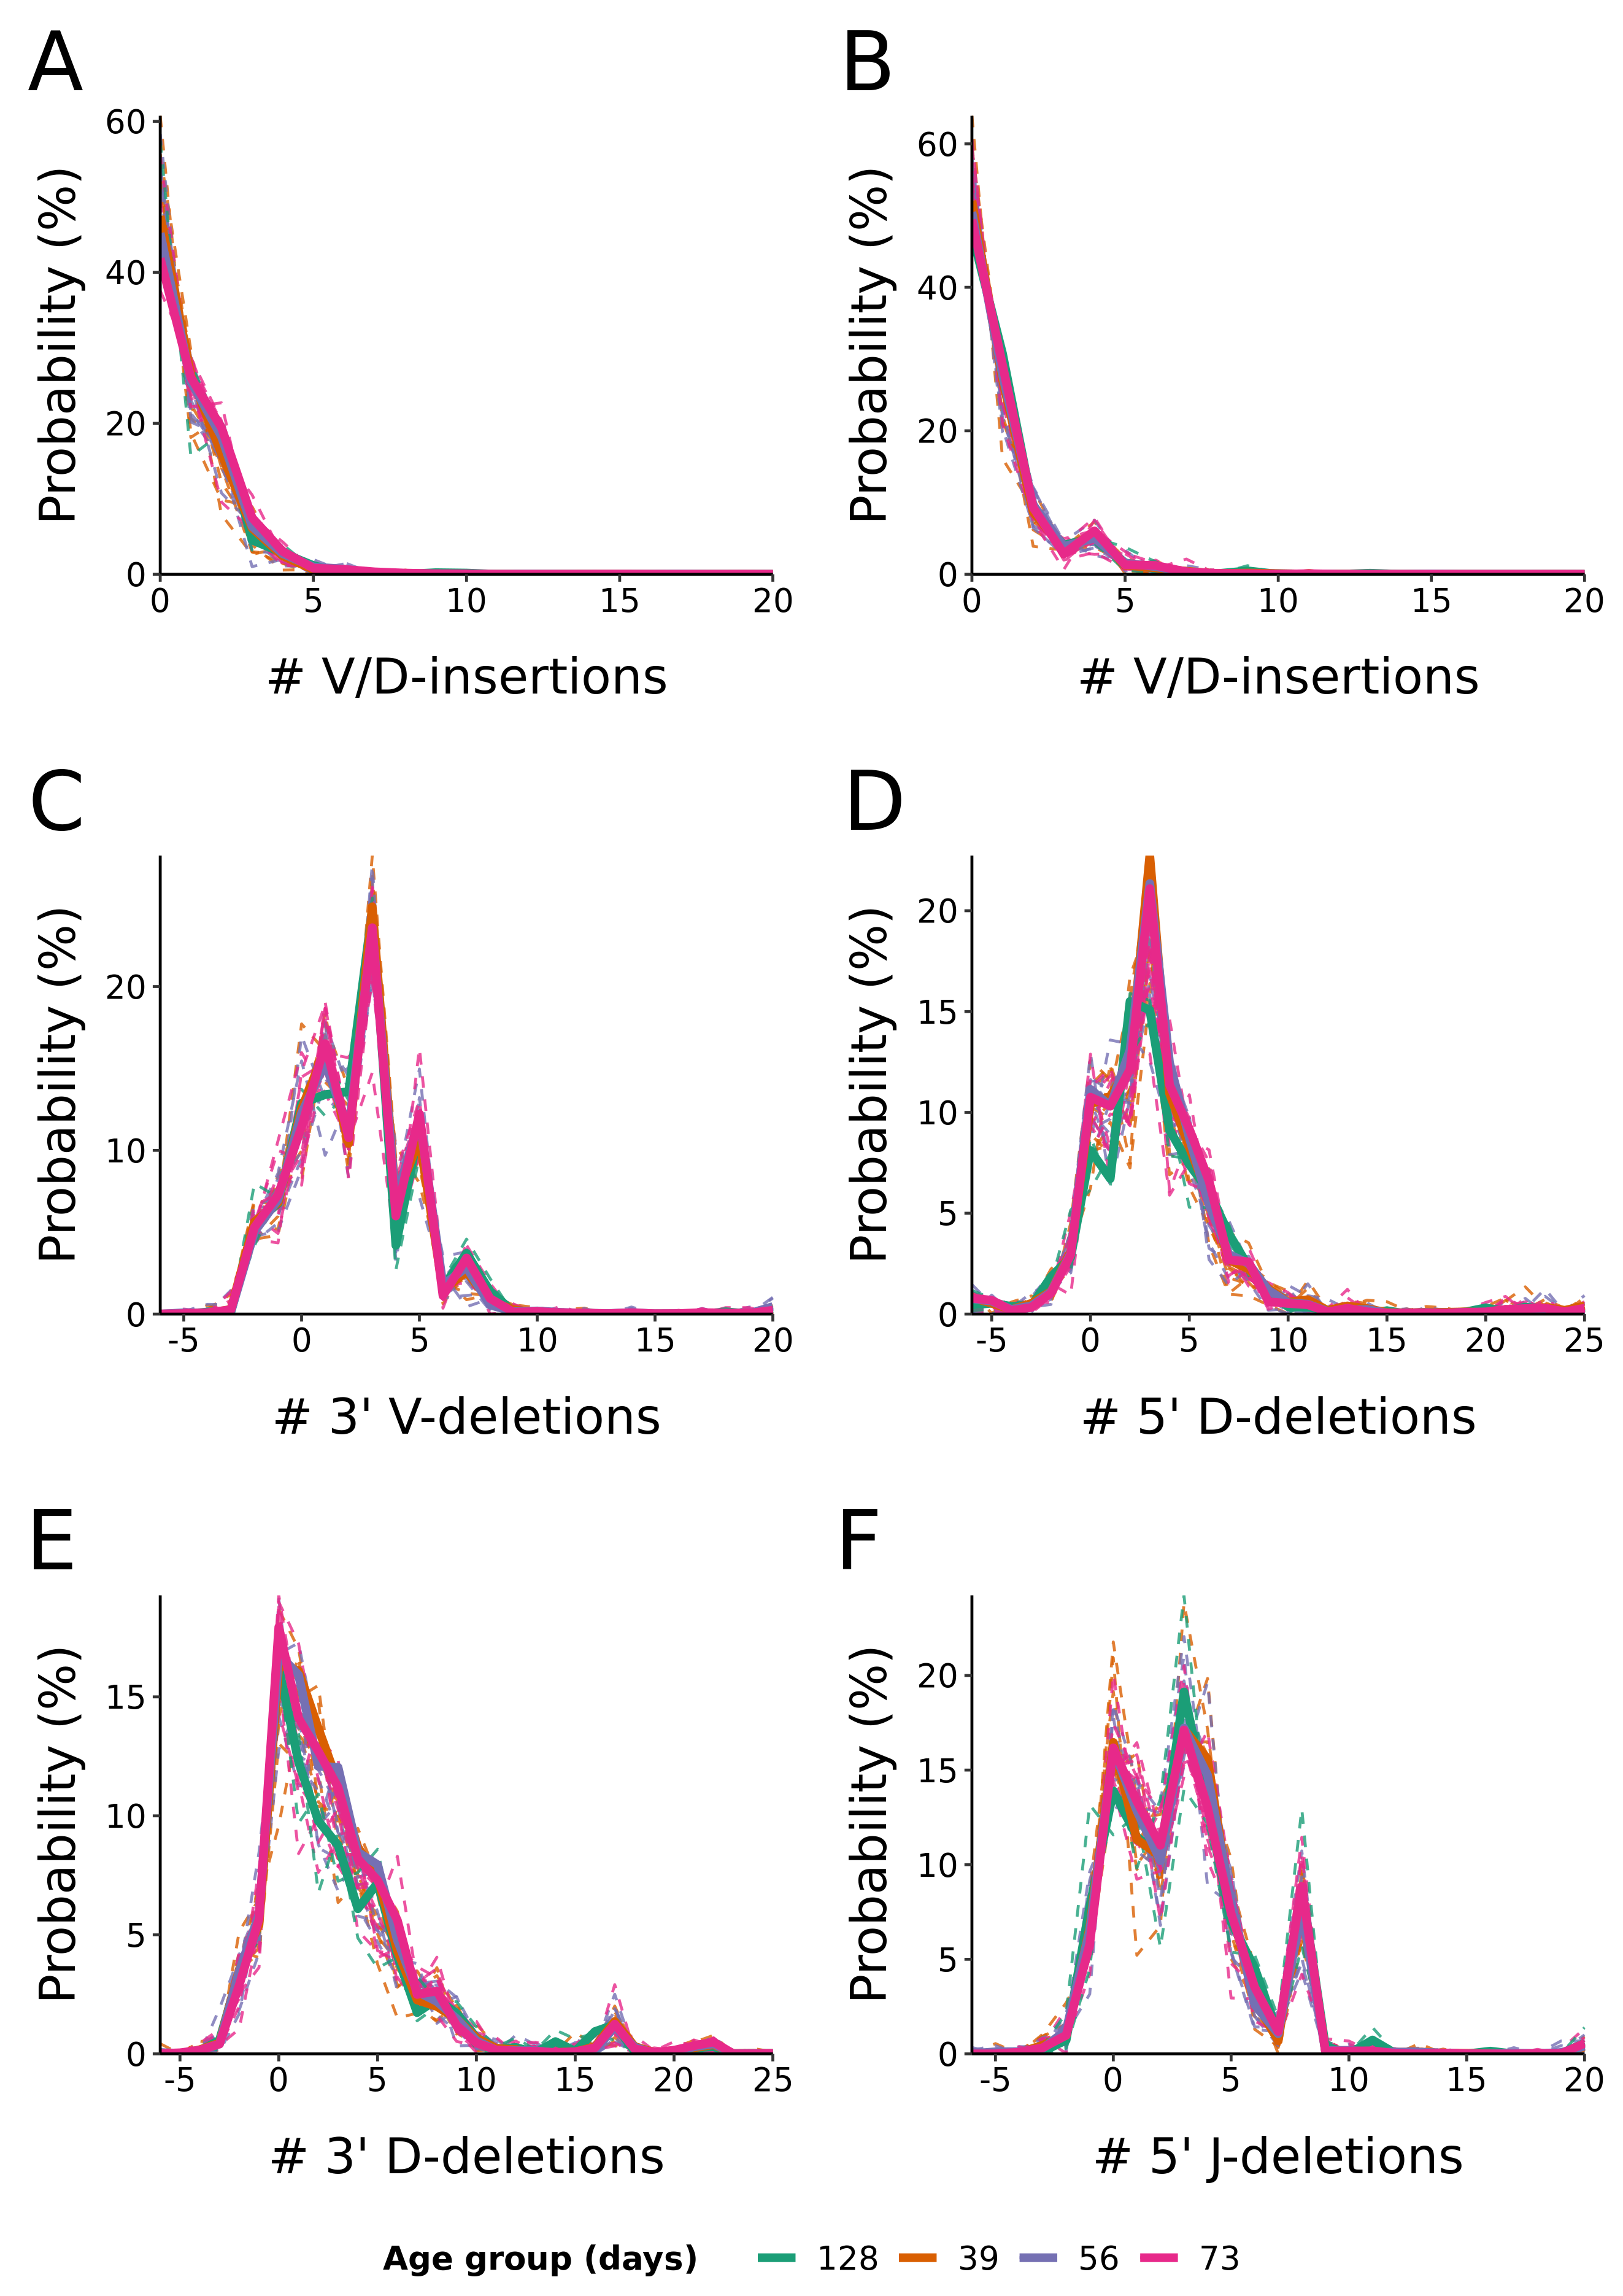
\includegraphics[width = 0.8\textwidth]{_Figures/png/ageing-igor-indels}
\begin{subfigure}{0em}
\phantomsubcaption{}
\label{fig:igseq-ageing-igor-indels-vdins}
\end{subfigure}
\begin{subfigure}{0em}
\phantomsubcaption{}
\label{fig:igseq-ageing-igor-indels-djins}
\end{subfigure}
\begin{subfigure}{0em}
\phantomsubcaption{}
\label{fig:igseq-ageing-igor-indels-vdel}
\end{subfigure}
\begin{subfigure}{0em}
\phantomsubcaption{}
\label{fig:igseq-ageing-igor-indels-d5del}
\end{subfigure}
\begin{subfigure}{0em}
\phantomsubcaption{}
\label{fig:igseq-ageing-igor-indels-d3del}
\end{subfigure}
\begin{subfigure}{0em}
\phantomsubcaption{}
\label{fig:igseq-ageing-igor-indels-jdel}
\end{subfigure}
\Caption{Generative insertion/deletion distributions in the \igseq ageing dataset}{Probability distributions of the number of N-insertions (A-B) or P-insertions/deletions (C-F) following VDJ recombination in adult male turquoise killifish of different ages, inferred from the \igseq ageing dataset using \program{IGoR}. P-insertions are modelled as negative deletions. Thin dashed lines represent the distributions inferred for individual killifish, while the thick solid lines represent those inferred from pooled data from all individuals in each age group.}
\label{fig:igseq-ageing-igor-indels}
\end{figure}

\begin{figure}
\centering
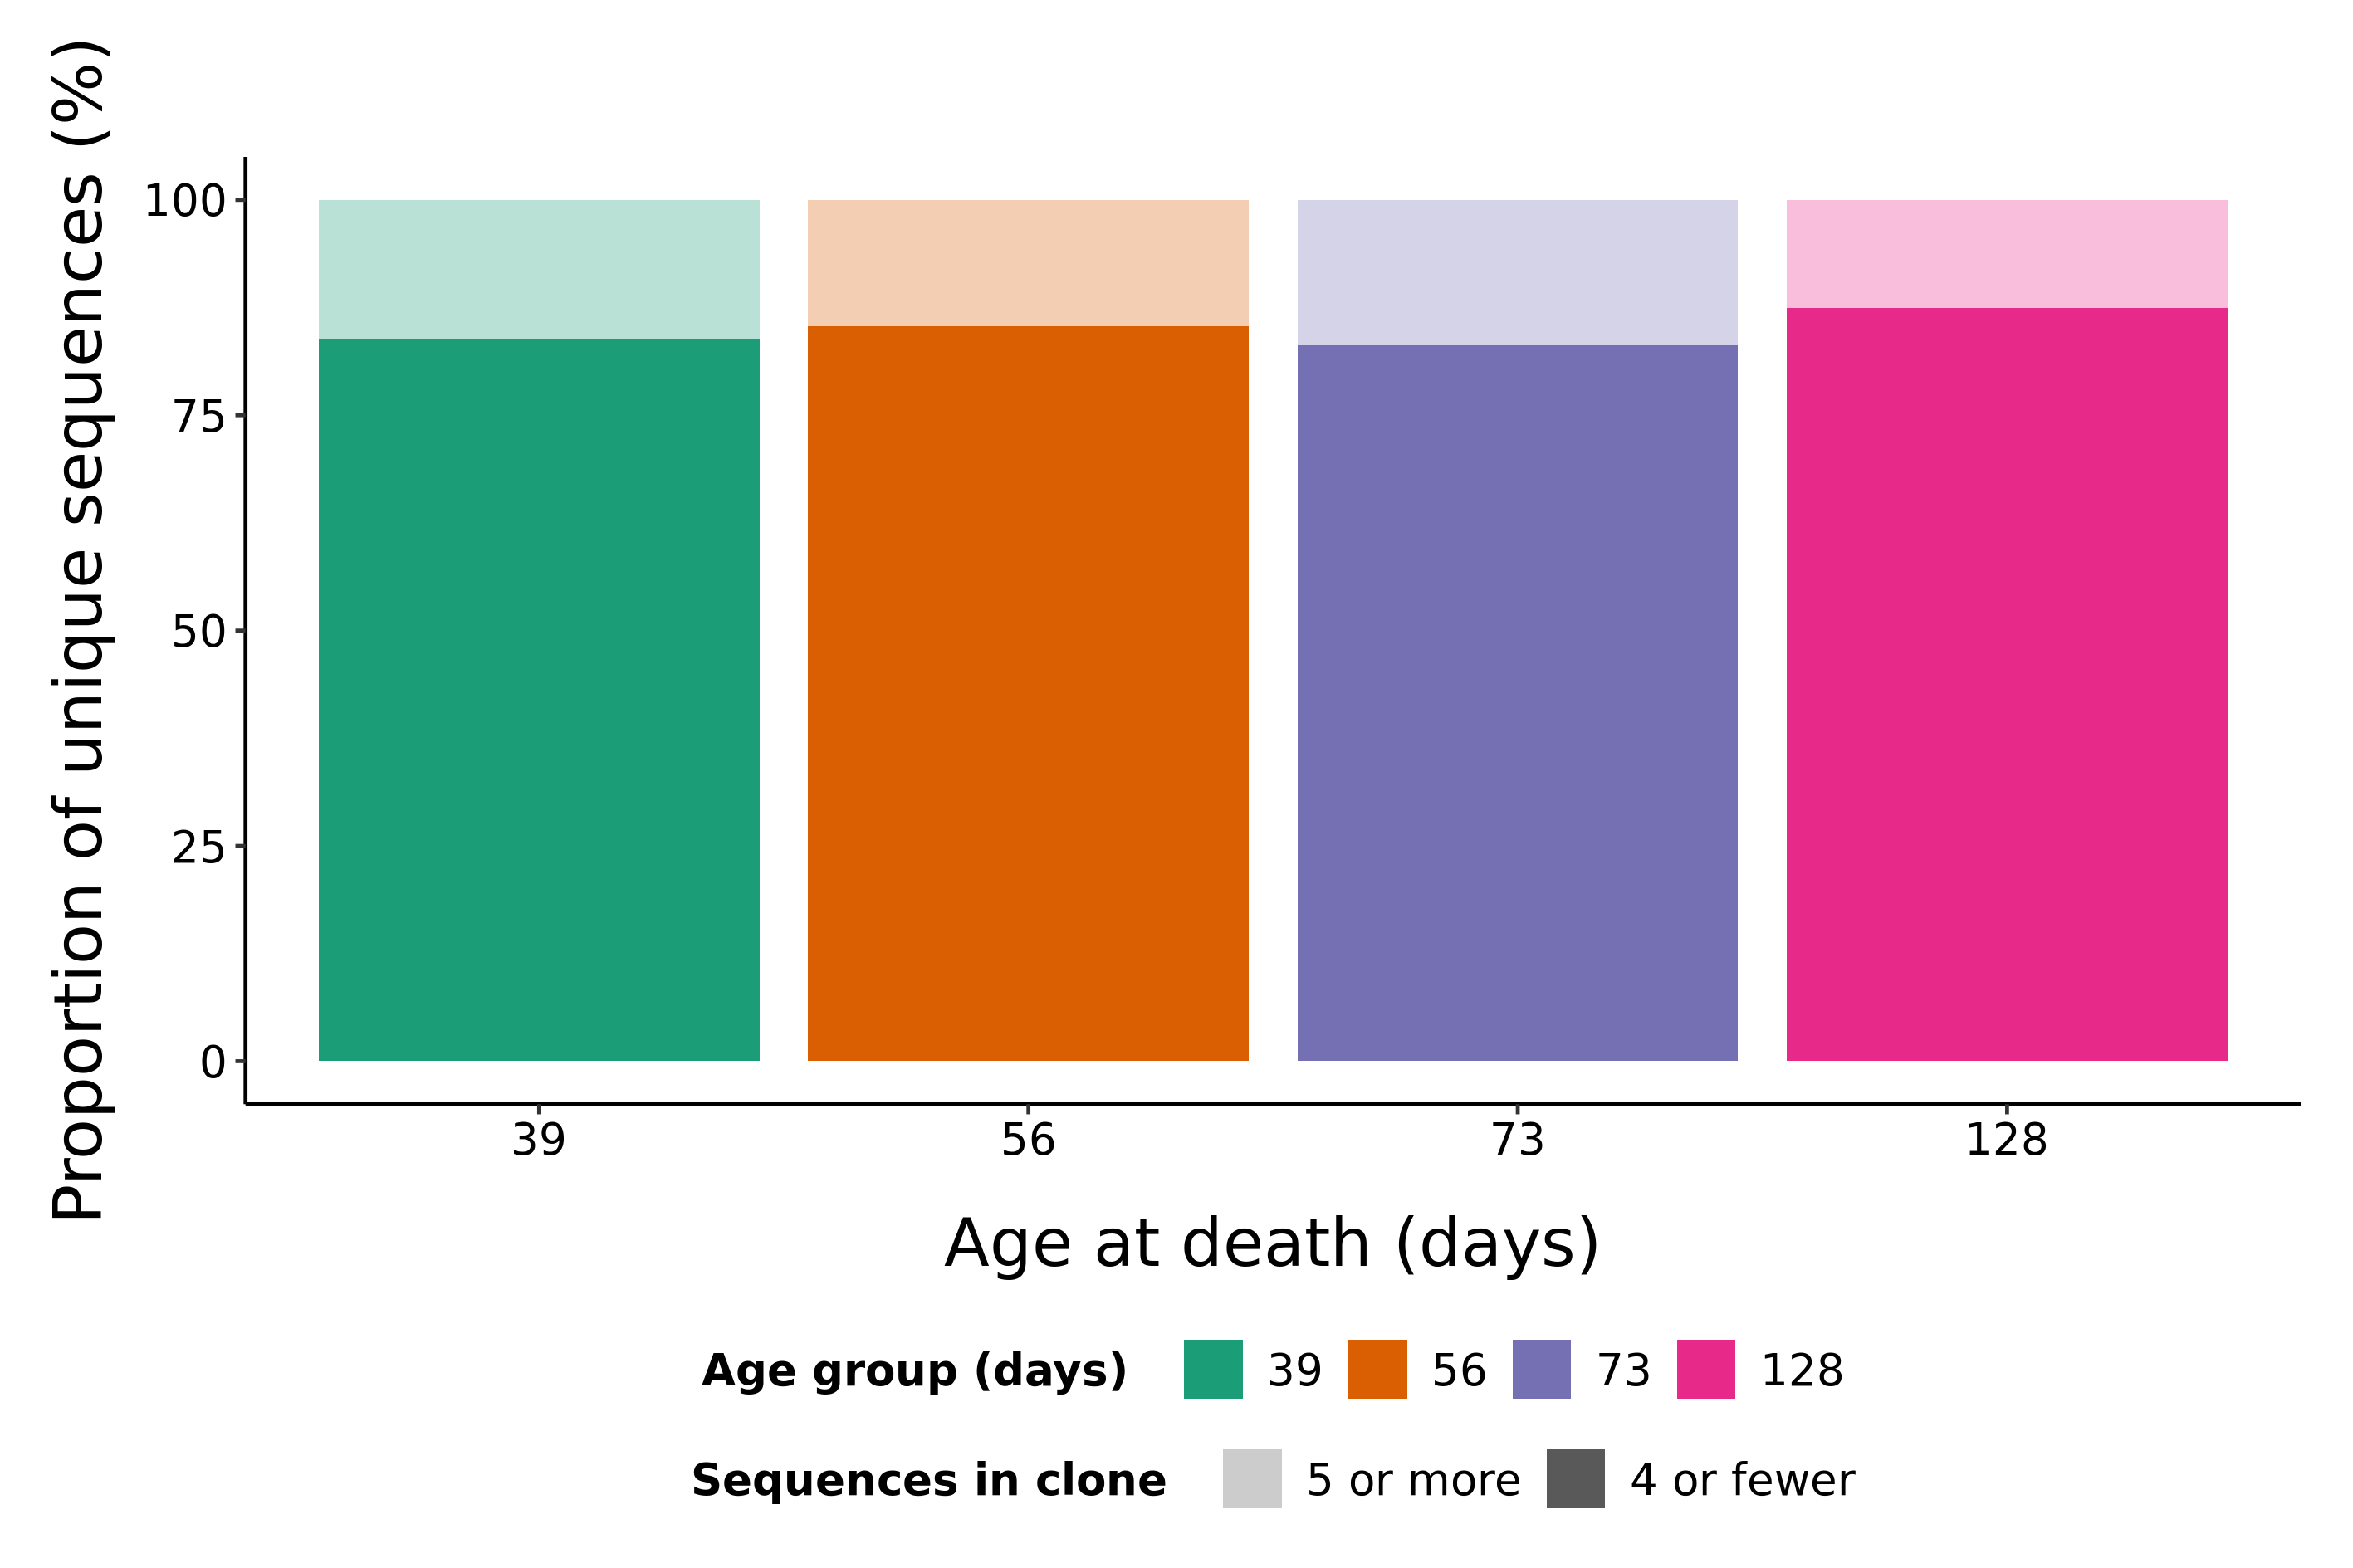
\includegraphics[width = 0.9\textwidth]{_Figures/png/ageing-pc-seq-in-small-clones}
\Caption{Proportion of unique sequences in large vs small clones in the \igseq ageing dataset}{Stacked barplots showing the mean proportion of unique sequences in large (5 or more unique sequences, top, pale) vs small (4 or fewer, bottom, dark) clones in each age group in the \igseq ageing dataset. The proportion of sequences in non-abundant clones does not change significantly with age (Kruskal-Wallis analysis of variance, $p=\embed{_Figures/txt/ageing-pc-seq-in-small-clones-kruskal-p.txt}$).}
\label{fig:igseq-ageing-pc-seq-in-small-clones}
\end{figure}

\begin{figure}
\centering
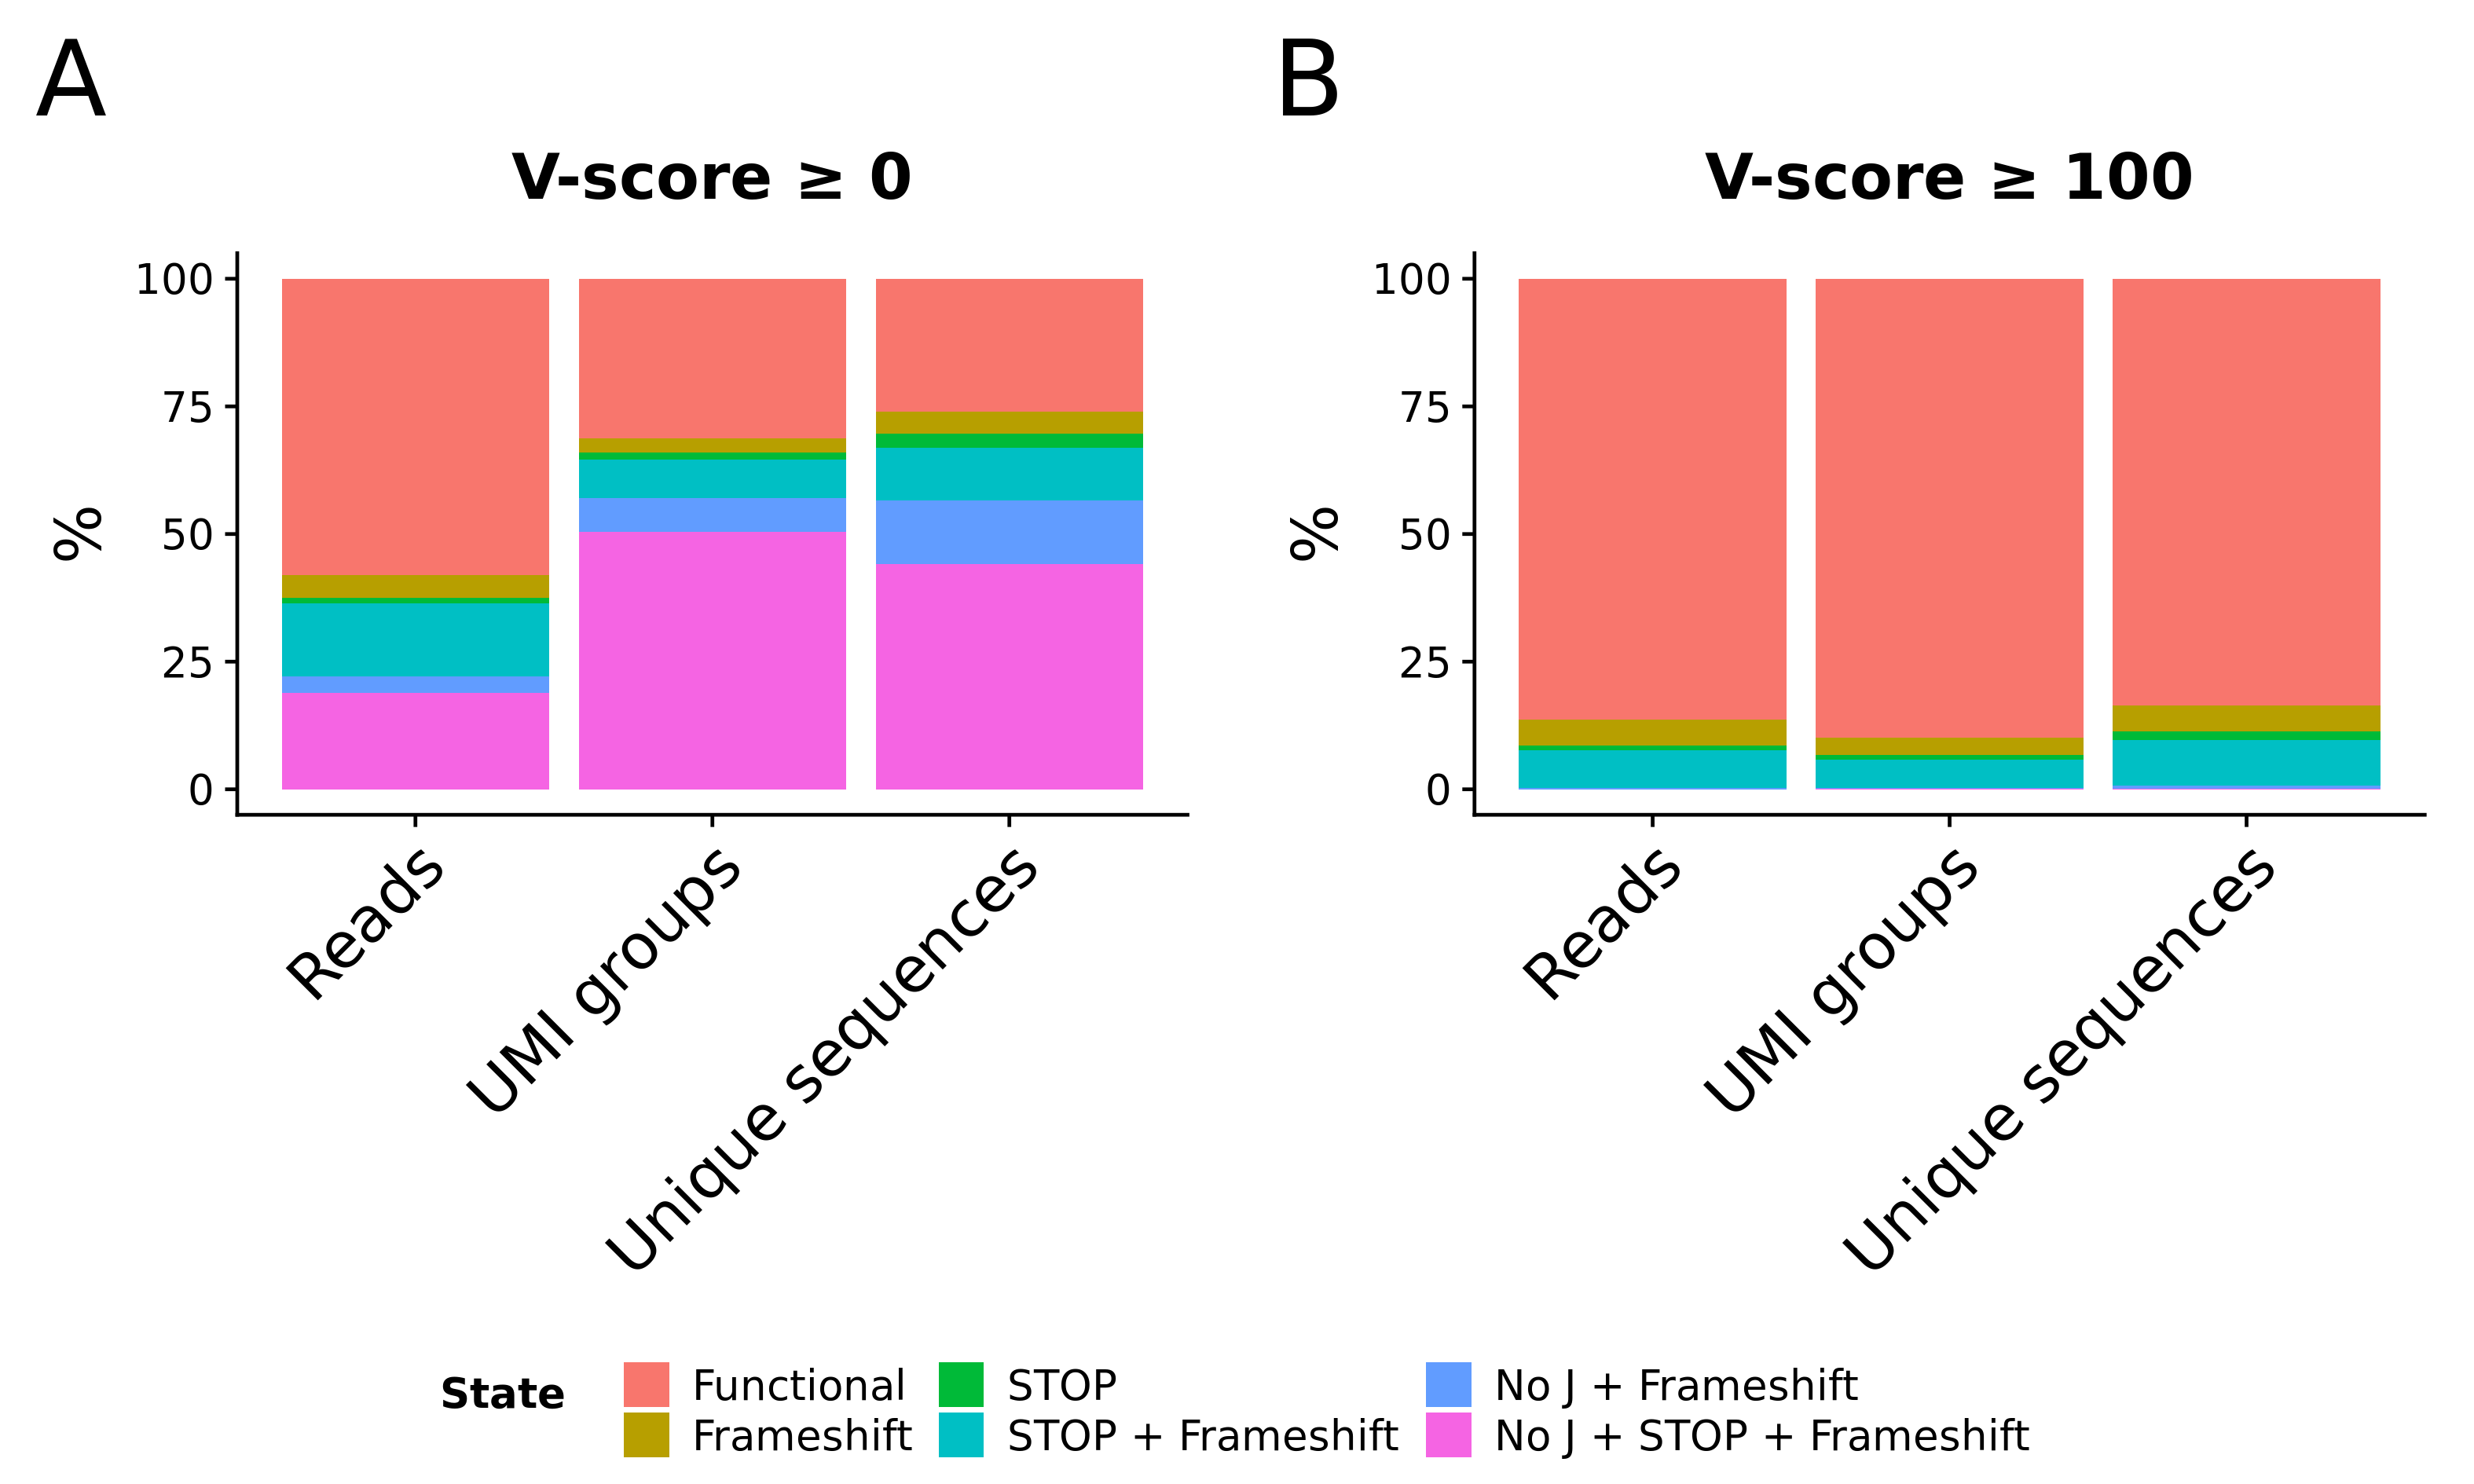
\includegraphics[width = 0.9\textwidth]{_Figures/png/gut-functional-prop}
\begin{subfigure}{0em}
\phantomsubcaption{}
\label{fig:igseq-gut-functional-prop-pre}
\end{subfigure}
\begin{subfigure}{0em}
\phantomsubcaption{}
\label{fig:igseq-gut-functional-prop-post}
\end{subfigure}
\Caption{Functional composition and V-score filtering in the \igseq gut dataset}{Proportion of input reads, UMI groups and unique sequences in the \igseq gut dataset belonging to different (non)functional categories, before (A) and after (B) filtering on V-alignment score.}
\label{fig:igseq-gut-functional-prop}
\end{figure}

\begin{figure}
\centering
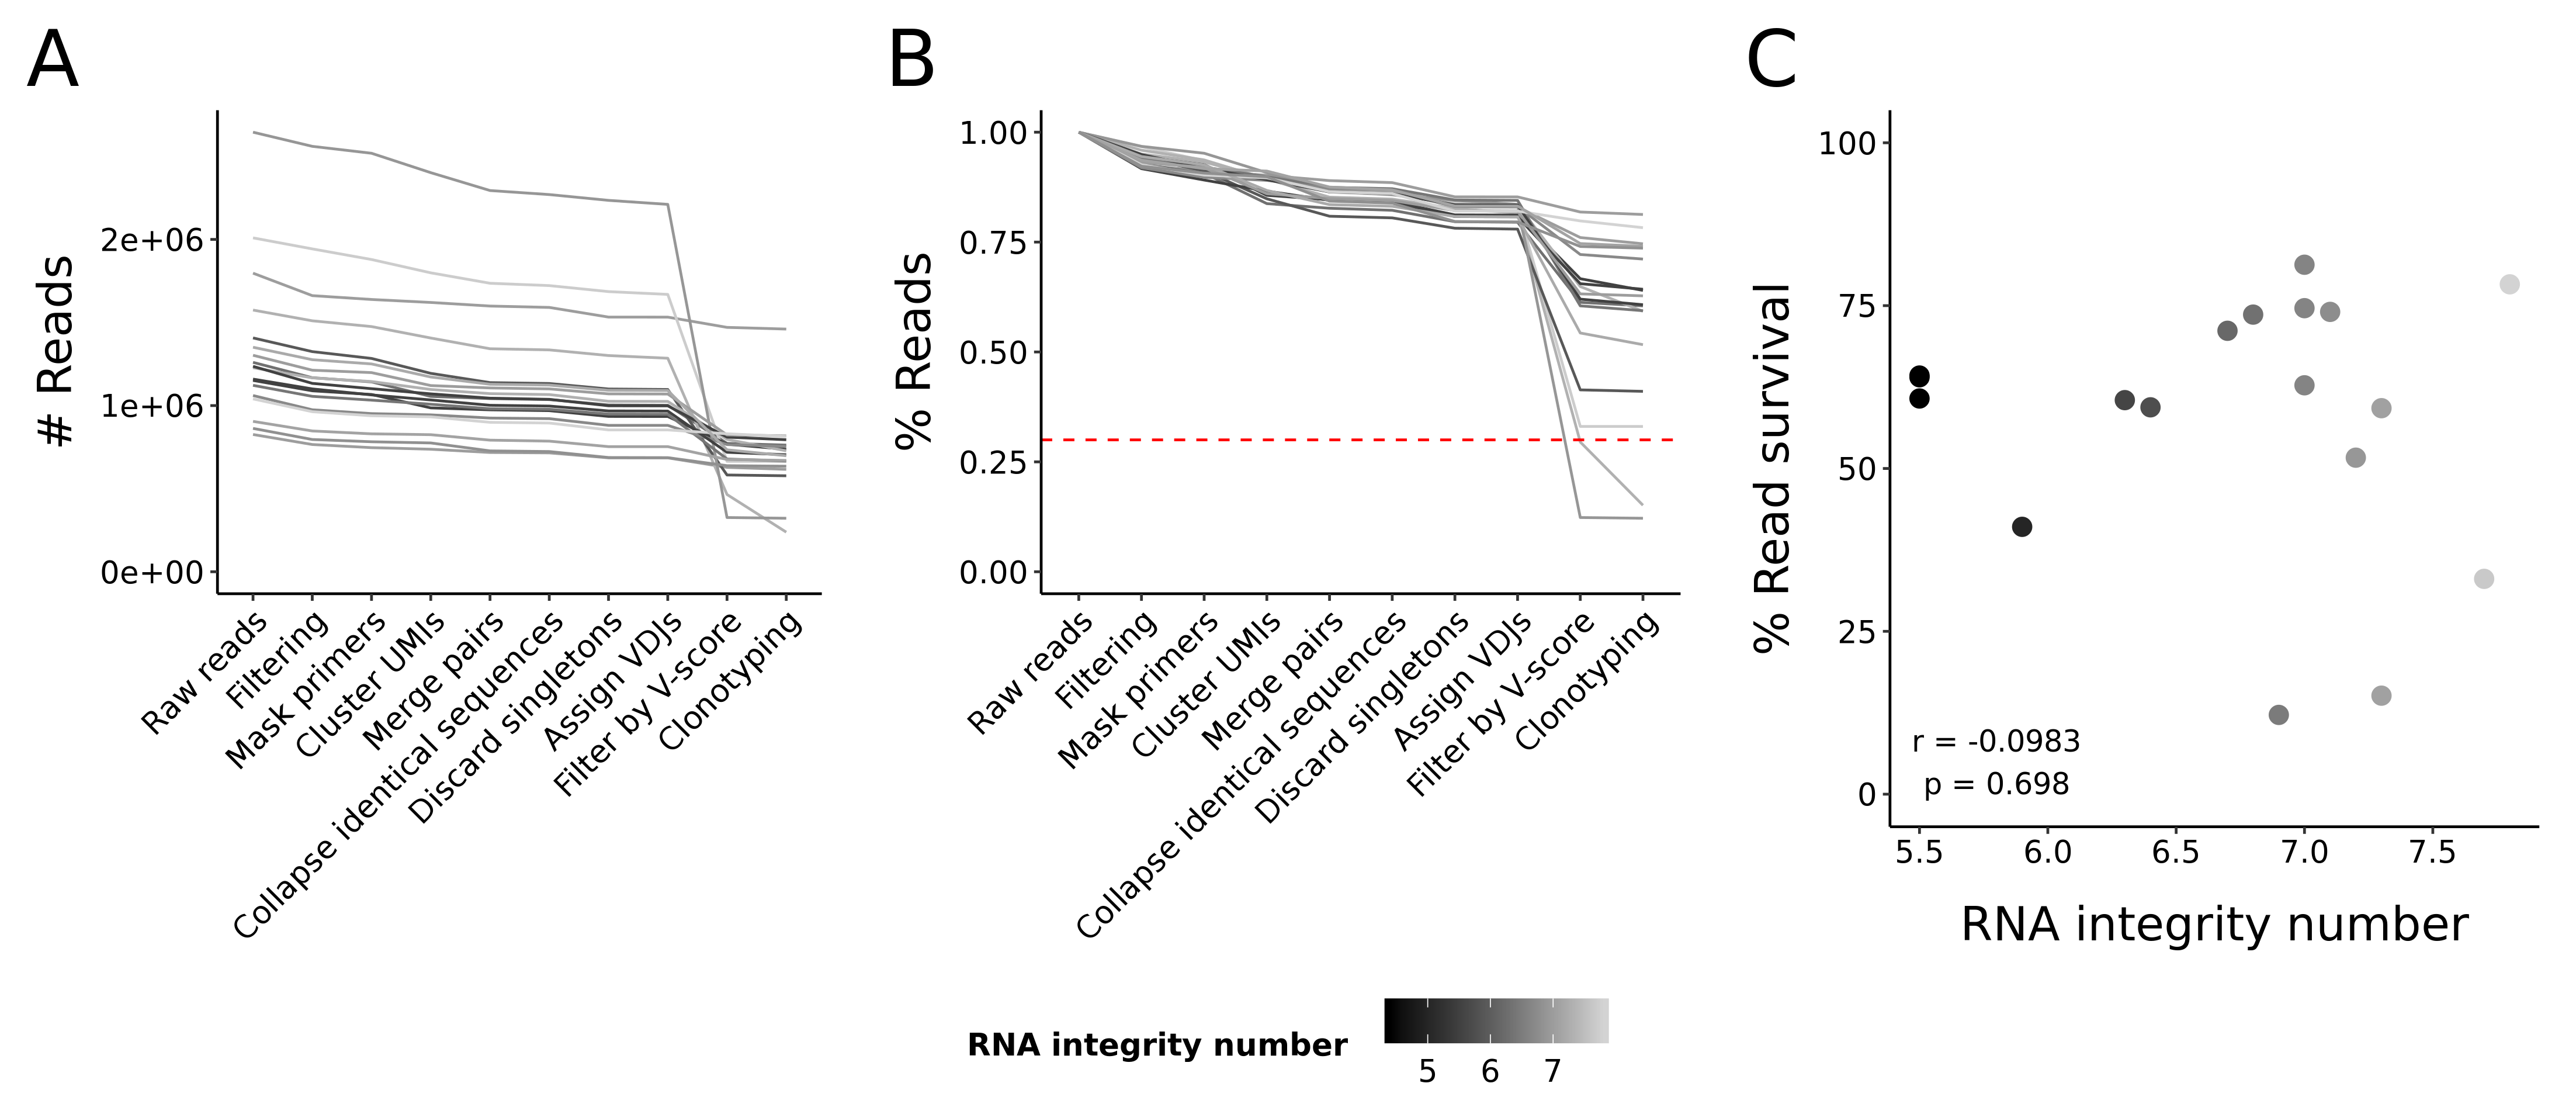
\includegraphics[width = \textwidth]{_Figures/png/gut-read-survival-all-rin.png}
\begin{subfigure}{0em}
\phantomsubcaption{}
\label{fig:igseq-gut-read-survival-all-rin-abs}
\end{subfigure}
\begin{subfigure}{0em}
\phantomsubcaption{}
\label{fig:igseq-gut-read-survival-all-rin-rel}
\end{subfigure}
\begin{subfigure}{0em}
\phantomsubcaption{}
\label{fig:igseq-gut-read-survival-all-rin-scatter}
\end{subfigure}
\Caption{Relationship between RNA integrity and read survival in the \igseq gut dataset}{(A-B) Absolute (A) and relative (B) read survival during pre-processing of the \igseq gut dataset, up to and including clonotyping, coloured by the RNA integrity number of each input sample. The dotted red line in (B) indicates the 30\% read-survival cutoff, below which samples were discarded prior to downstream analysis. (C) Scatterplot of RNA integrity number vs percentage read survival, up to and including clonotyping.}
\label{fig:igseq-gut-read-survival-all-rin}
\end{figure}

\begin{figure}
\centering
\begin{subfigure}{0em}
\phantomsubcaption{}
\label{fig:igseq-gut-clone-diversity-solo-spectra-age}
\end{subfigure}
\begin{subfigure}{0em}
\phantomsubcaption{}
\label{fig:igseq-gut-clone-diversity-solo-spectra-groups}
\end{subfigure}
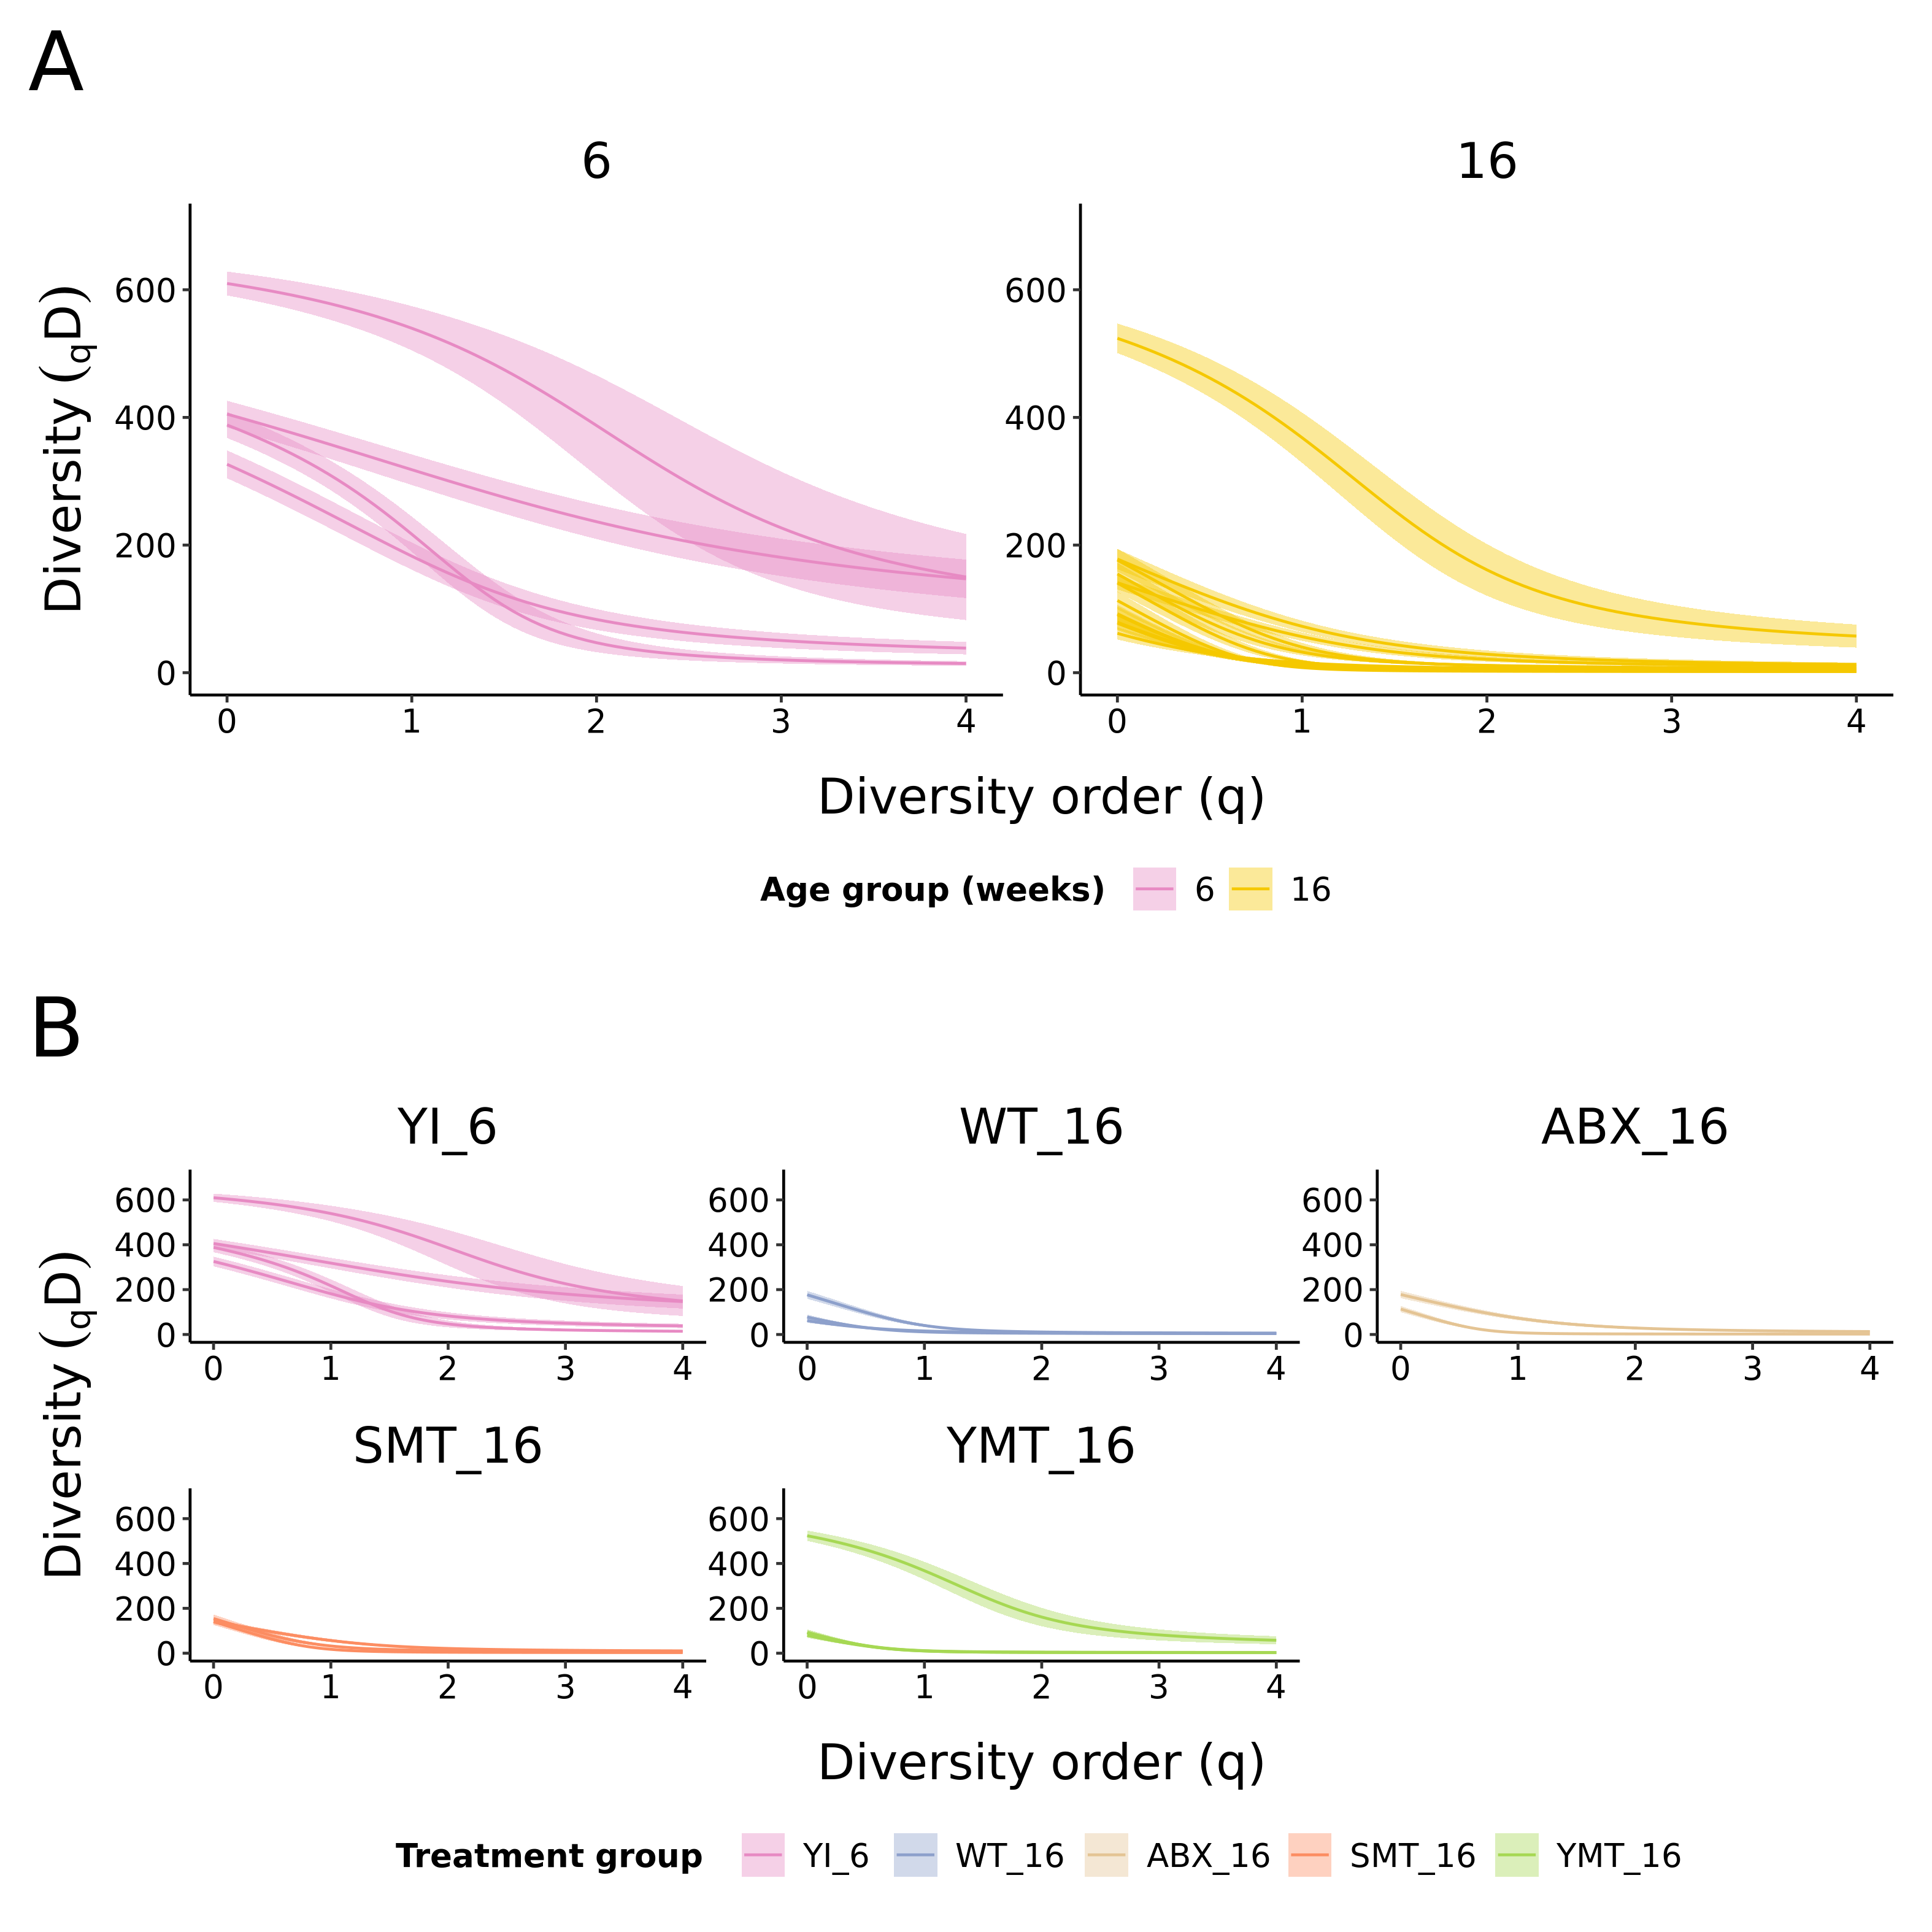
\includegraphics[width = 0.8\textwidth]{_Figures/png/igseq-gut-clone-diversity-solo-spectra}
\Caption{Per-individual clonal-diversity spectra for the \igseq gut dataset}{Hill diversity spectra of clone sizes (as measured by number of unique sequences per clone) for each individual in the \igseq gut dataset, grouped by (A) age at death and (B) treatment group.}
\label{fig:igseq-gut-clone-diversity-solo-spectra}
\end{figure}

\begin{figure}
\centering
\begin{subfigure}{0em}
\phantomsubcaption{}
\label{fig:igseq-gut-vj-diversity-solo-spectra-age}
\end{subfigure}
\begin{subfigure}{0em}
\phantomsubcaption{}
\label{fig:igseq-gut-vj-diversity-solo-spectra-groups}
\end{subfigure}
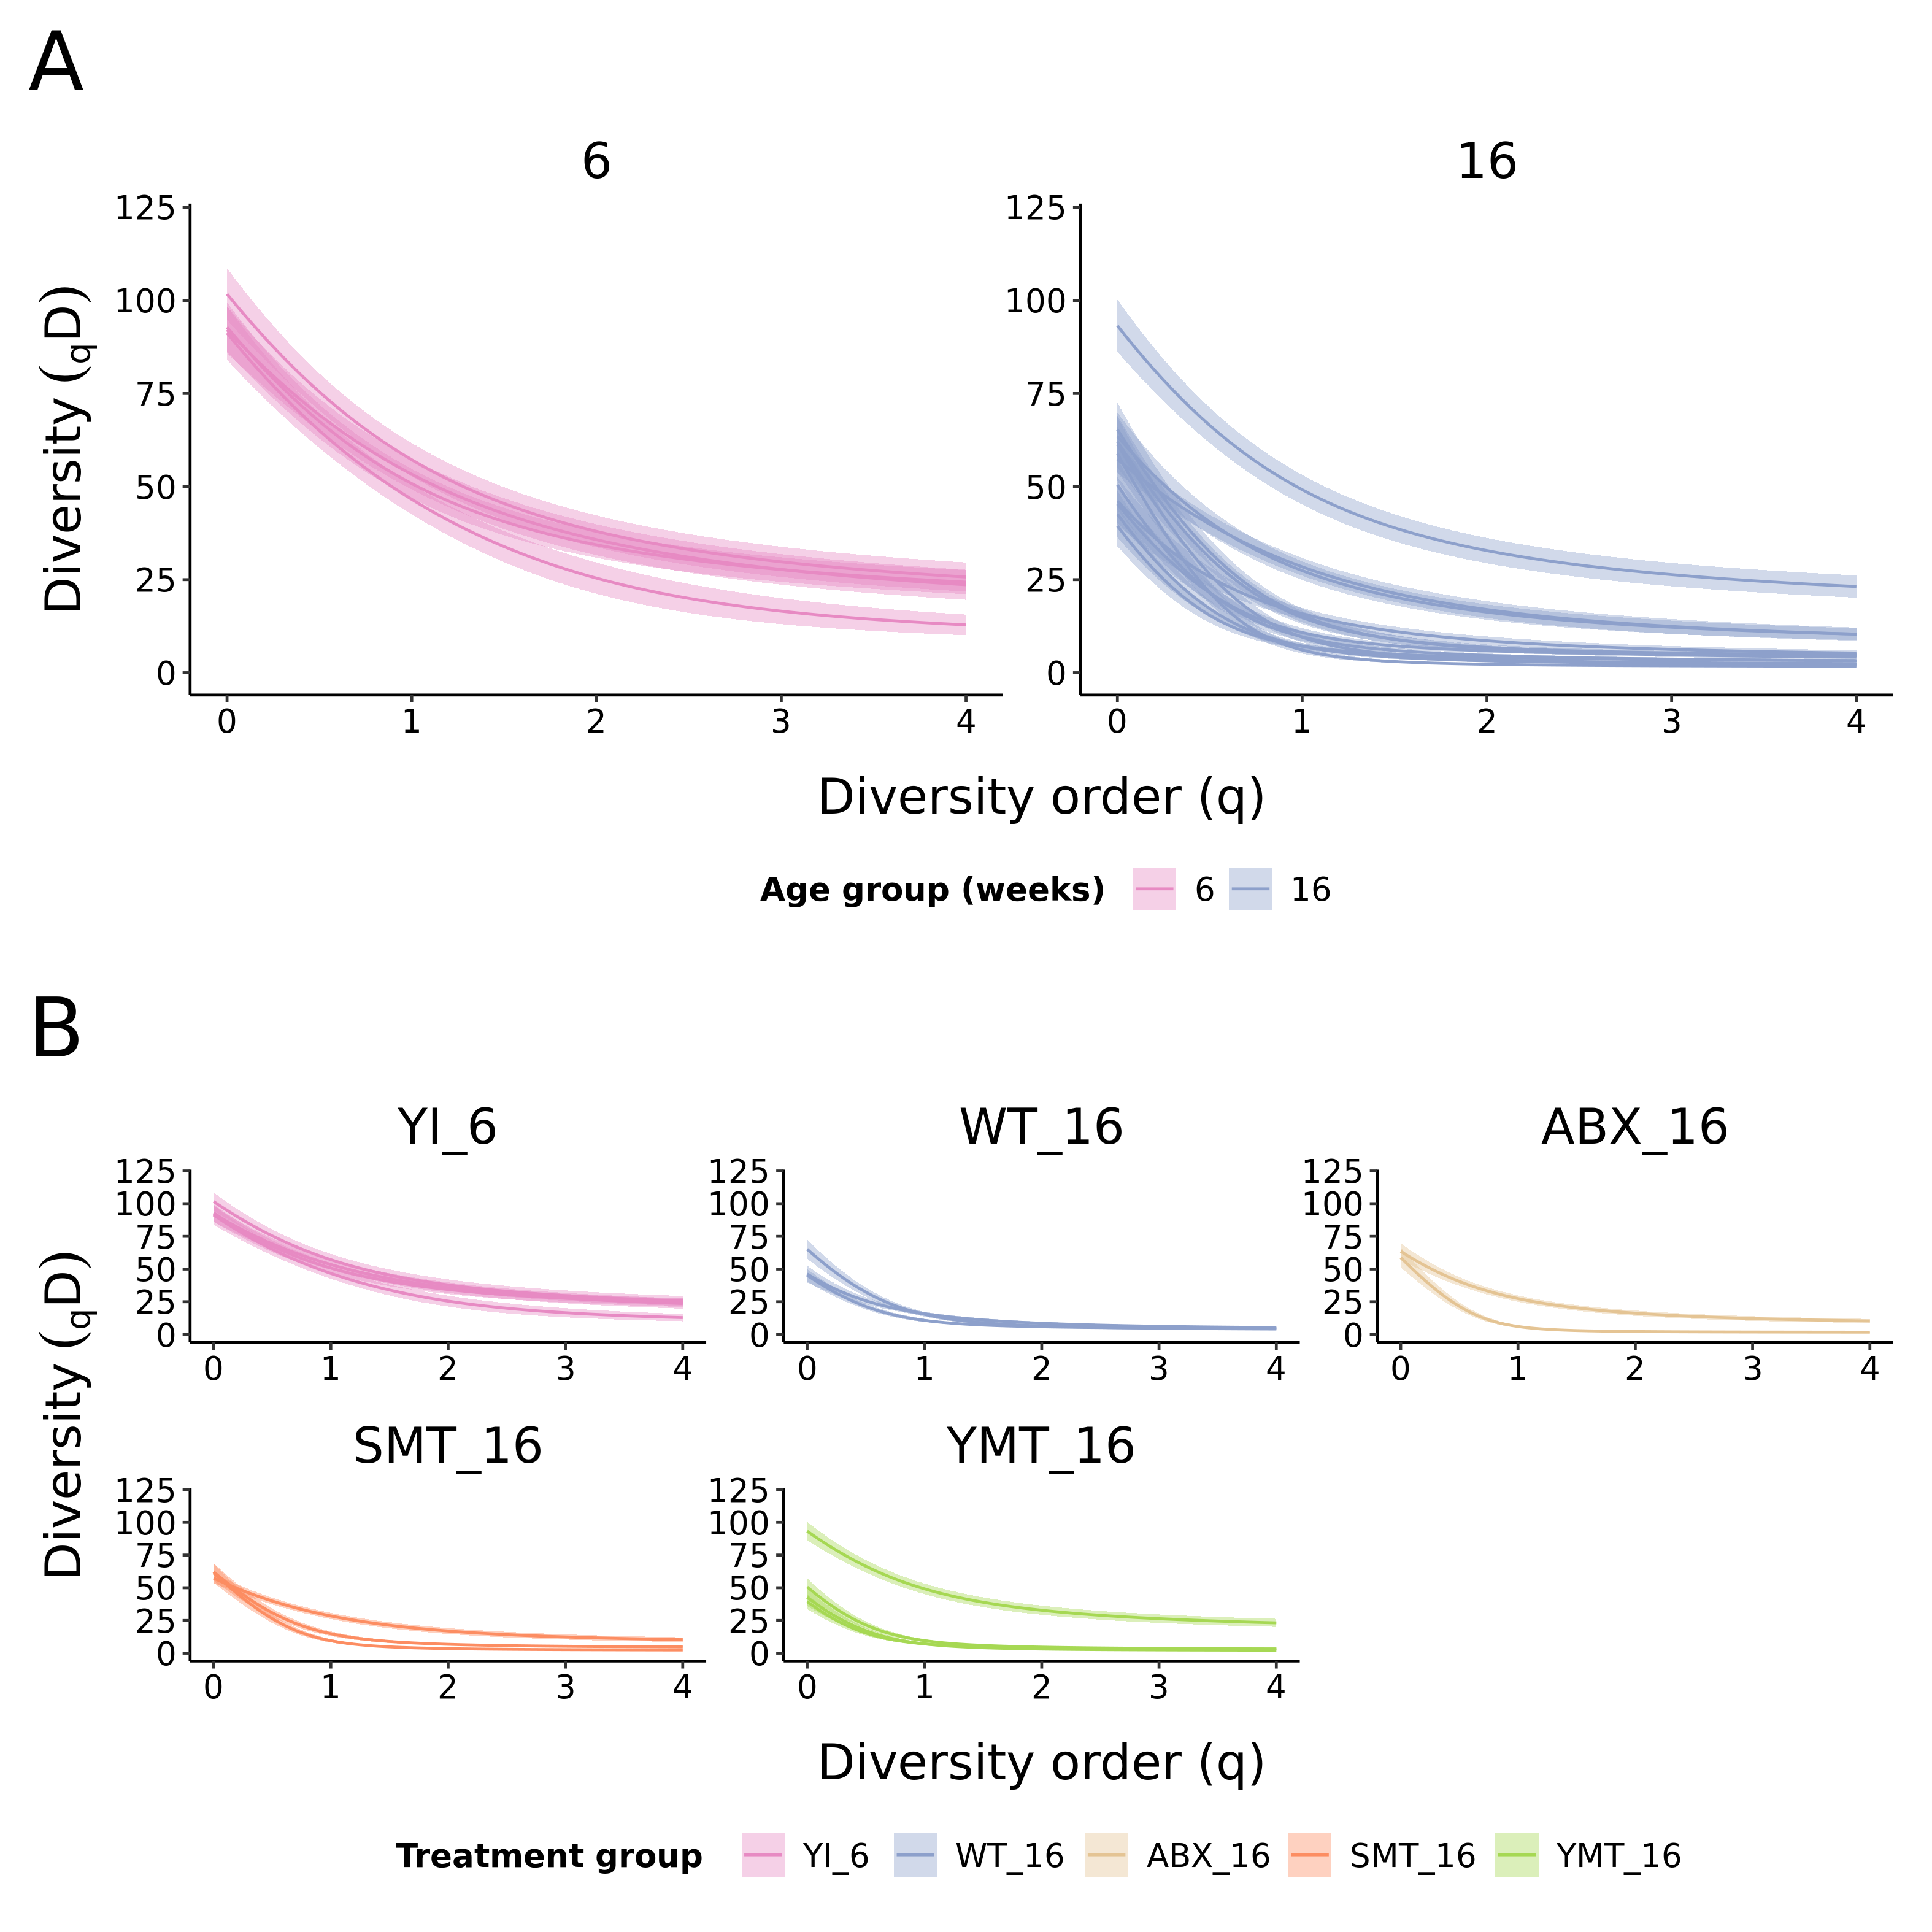
\includegraphics[width = 0.8\textwidth]{_Figures/png/igseq-gut-VJ-diversity-solo-spectra}
\Caption{Per-individual VJ-diversity spectra for the \igseq gut dataset}{Hill diversity spectra of VJ usage (as measured by number of unique sequences per V/J combination) for each individual in the \igseq gut dataset, grouped by (A) age at death and (B) treatment group.}
\label{fig:igseq-gut-vj-diversity-solo-spectra}
\end{figure}
